\documentclass[a4j , 11pt , twoside]{jbook}
\usepackage{ascmac} % プログラムリスト等を囲むボックスのため
\usepackage{matx} % MaTXのロゴ(例)「\MaTX{}を用いた制御系設計」
\usepackage{manyfloat} % 1ページに多くの図や表をまとめるため
\usepackage{docmute}
\usepackage{amsmath}
\usepackage{ascmac}
\usepackage{fancybox}
\usepackage[dvipdfmx]{graphicx}% ポストスクリプトファイルを取り込むため
\usepackage{url}
\usepackage{color}
\begin{document}
%-----------------------------------------------------------
% タイトルページ
\title{倒立振子の安定化制御}
\author{渡部僚太}
\date{2018年7月2日}
\maketitle
%-----------------------------------------------------------
% 目次
\pagenumbering{roman} %ページ番号をローマ数字に設定
\tableofcontents % 目次
\listoffigures % 図の目次
\listoftables % 表の目次
\cleardoublepage % 次ページが表ページになるように改ページ
\pagenumbering{arabic} % ページ番号をアラビア数字に設定
%-----------------------------------------------------------------
% 本文
\chapter{報告書を書く上で(後で消す)}
	\section{注意点}
完成したら必ずこの部分はmainから削ってください

\section{倒立振子の全体の流れ}
以下に今回行った倒立振子に関する実験及びシミュレーションなどの流れを示す\\
\\
1.倒立振子のモデリングと自由応答シミュレーション(B.倒立振子の安定化制御、制御工学実験第3\ 倒立振子の安定化制御の資料も含む)\\
2.倒立振子のパラメータ同定と検証\\
3.設計(線形)モデルの決定とシステム解析\\
4.制御系の設計1(状態フィードバック)と制御性能評価\\
5.制御系の設計2(最小次元オブザーバ)と制御性能評価\\
6.制御系の設計3(コントローラの離散化)と制御性能評価\\
7.制御系の設計4(振り上げ制御・安定化)と制御性能評価\\
8.倒立振子の制御実験(安定化制御)\\
9.倒立振子の制御実験(目標値の変更)\\
10.倒立振子の制御実験(振り上げ制御・安定化)\\
11.教育機関報告書作成(その1)\\
\\
以上を分割を以下のグループに分けることで今までしてきたことがどのチャプターにかかれるかを示す\\
\\
A:はじめに\ この実験を行う背景とか\\
B:モデリング\ 1,\ 2,\ 3,\\
\\
C:制御系設計\ 4,\ 5,\ 6,\ 7\\
\\
D:シミュレーション\ 1,\ 2,\ 4,\ 5,\ 6,\ 7,\ 8,\ 9,\ 10\\
\\
E:実験\ 8,\ 9,\ 10\\
F:おわりに\ 学んだこととか\\
G:プログラム\ 

\section{疑問}
質問コーナー\\

・シミュレーションの部分は今までやってきたシミュレーションすべてを書かなければならないか\\
→最低限実験と比較したシミュレーションは必要。それ以外は任意でよい。必要最低限のせればよい\\
・制御系の設計などでMaTX,Java,JaMOXの3通りからアプローチをかけたが報告書にはそのすべてを記載末うべきか\\
→任意でよい。でもjamoxのブロック線図は乗せたほうが良い\\
・付録のプログラムについても同様で3通りのプログラムやブロック線図を貼り付けるべきか\\
→任意でよい\\
・\\
・\\
・\\
・\\
・\\
・\\
・\\
・\\
・\\
・\\
・\\

\section{トラブルシューティング}
トラブルシューティング!困ったときはここを見てね\\
・図においてlabelとrefを対応させるときにはlabelをcaptionの下に置く必要がある\\
・改ページを行うにはnewpageを用いる\\
・改段落にはparを用いる\\
・\\
・\\
・\\
・\\
・\\
・\\
・\\
・\\


\chapter{はじめに}
	\section{実験目的}
本実験の目的は、倒立振子の安定化制御の制御系の設計を状態空間法を用いて行うことにより、線形時不変システムを設計することである。
具体的には以下の
\begin{itemize}
	\item 振子を垂直上向きに配置した状態から実験を開始し、安定化制御を行う。また、このとき十数度角度を傾けても安定化制御を行えるようにする。(不安定平衡点の安定化)
	\item 安定化制御を行っている状態でパルス入力を加え、台車の位置が変わっても安定化制御を行えるようにする。
	\item 振子を下向きに配置した状態から振り上げ、安定化制御を行えるようにする。
\end{itemize}
を達成することが目的である。\cite{Koga:Binpe}
\par
不安定平衡点とは、倒立振子系における平衡点の1つである。今回実験で使用する倒立振子系には平衡点が2つ存在する。1つは棒が鉛直線に沿って垂れ下がった状態、もう1つは棒が鉛直線に沿って倒立した状態である。前者は
振子を揺らした場合、時間が立てば止まる安定平衡点である。後者は振子を揺らした場合、そのまま振子が真っ逆さまに落ちていく不安定平衡点である。
\newpage

\section{制御対象}
\subsection{倒立振子系}
本実験で用いる倒立振子系を以下に載せる。
また、実際に実験で用いる倒立振子系の写真も載せる。
\begin{figure}[H]
	\centering
	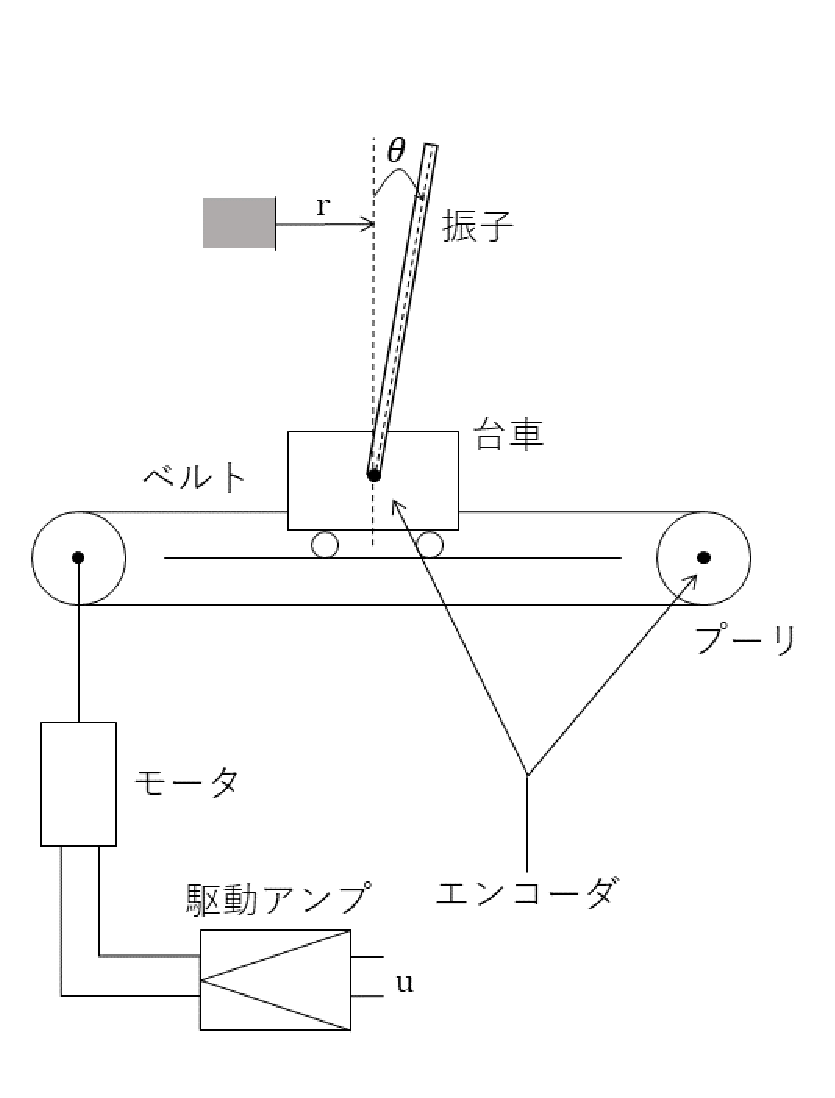
\includegraphics[width=0.6\linewidth]{gazo/pendulum.eps}
	\caption{倒立振子系}
	\label{image:pendulum}
\end{figure}
\begin{figure}[H]
	\centering
	\includegraphics[width=10cm,pagebox=cropbox,clip]{gazo/Pendulum.pdf}
	\caption{倒立振子系(写真)}
	\label{image:pendulum_photo}
\end{figure}
図\ref{image:pendulum}は倒立振子系を表す図である。モノレールの上に台車が置かれ、台車上のモノレールと直角な軸に一本の棒が取り付けられ、棒はその軸まわりに自由に回転できる。台車はベルトとプーリを介して、モータにより駆動され、
モノレール上を走行できる。すなわち、棒(振子)は鉛直線とモノレールにより定まる平面に拘束されて、台車によって動かされるようになっている。\\
\subsection{観測出力と操作入力}
倒立振子系の観測出力として、エンコーダにより、つぎの2つが測定できる。\\
\begin{itemize}
  \item 台車の基準位置から変位$r$に比例する電圧$y_{1}$
  \item 棒の鉛直線となす角度$\theta$に比例する電圧$y_{2}$
\end{itemize}
一方、操作入力は、つぎのものである。
\begin{itemize}
  \item モータの駆動アンプの入力電圧$u$
\end{itemize}
ここで、モータにより駆動される台車には、$u$に比例した駆動力が働くものとする。



\chapter{モデリング}
	\section{倒立振子のモデリング}
実験目的を達成する制御システムを設計するためにまず、倒立振子系について、状態方程式と観測方程式から成る数式モデルを導出する。
\subsection{状態方程式}
	\begin{figure}[H]
		\centering
		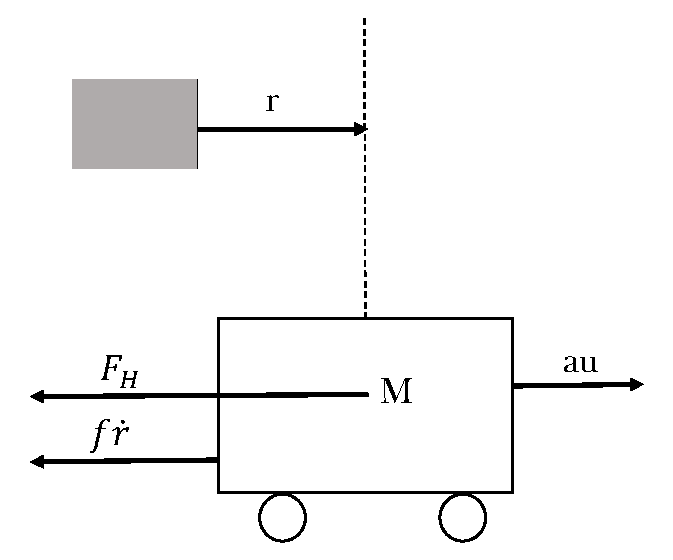
\includegraphics[width=0.4\linewidth]{gazo/cart.eps}
		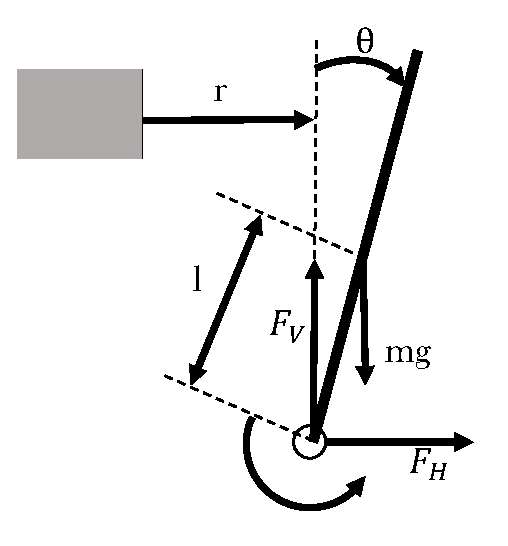
\includegraphics[width=0.4\linewidth]{gazo/stick.eps}
		\caption{数式モデル導出のための参考図}
		\label{image:reference}
	\end{figure}	
	図\ref{image:reference}を参考に各運動方程式を導出すると、\\
	台車の運動方程式は\\
	
	\begin{equation}
		M\ddot{r}=au-F_{H}-f\dot{r}
		\label{eq:motion_eq_cart}
	\end{equation}
	
	倒立振子の回転の運動方程式は
	
	\begin{equation}
		J\ddot{\theta}=lF_{V}\sin \theta -lF_{H}\cos \theta -c\dot{\theta}
		\label{eq:rotemotion_eq_stick}
	\end{equation}
	\\
	倒立振子の水平方向の運動方程式は
	
	\begin{equation}
		m\frac{d^{2}}{dt^{2}}(r+l\sin\theta) = F_{H}
		\label{eq:horizonmotion_eq_stick}
	\end{equation}
	倒立振子の垂直方向の運動方程式は
	
	\begin{equation}
		m\frac{d^{2}}{dt^{2}}(l\cos\theta) = F_{V}-mg
		\label{eq:vertical_eq_stick}
	\end{equation}
	
	となる。
	\par
	ここで各式の導出過程を述べる。図\ref{image:reference}より台車の運動方程式は、振り子からの水平抗力$F_{H}$を考慮してニュートンの第二法則より(\ref{eq:motion_eq_cart})
	式を導くことができる。
	ただし、$M$は台車の質量、$f$は台車の摩擦係数、$a$は駆動アンプへの入力電圧から台車への駆動までのゲイン、$u$はモータの駆動アンプへの入力電圧、$r$は台車の基準位置からの変位である。
	同様にニュートンの第二法則を用いることでそれぞれの方向における(\ref{eq:horizonmotion_eq_stick}),(\ref{eq:vertical_eq_stick})式の運動方程式を導くことができる。
	ただし、$m$は振り子の質量、$l$は回転軸・重心間の距離、$g$は重力加速度、$F_{V}$は振り子が台車から受ける垂直抗力である。
	また、$\theta$は鉛直上向きを$\theta=0$としたときの角度である。
	\par
	最後に(\ref{eq:rotemotion_eq_stick})式は回転に対する運動方程式を考えることで上記と同様に求めることができる。
	ただし、$J$は重心回りの慣性モーメント、$c$は回転軸摩擦係数である。
	\par
	いま、4つの状態変数から成るベクトル、すなわち状態$x$を
					
	\[
		x=\left[
		\begin{array}{ccc}
			r\\
			\theta\\
			\dot{r}\\
			\dot{\theta}\\
		\end{array}
		\right]
		\label{eq:array1}
	\]
					
	のように定義し、(\ref{eq:motion_eq_cart})式,(\ref{eq:rotemotion_eq_stick})式,(\ref{eq:horizonmotion_eq_stick})式,(\ref{eq:vertical_eq_stick})式
	から倒立振子系の非線形状態方程式を求める。
	
	\begin{eqnarray}
		\dot{x} = f(x,u) = \left[
		\begin{array}{ccc}
			\dot{r}\\
			\dot{\theta}\\
			\ddot{r}\\
			\ddot{\theta}\\
		\end{array}
		\right]
		\label{eq:array2}
	\end{eqnarray}
					
	ここで(\ref{eq:horizonmotion_eq_stick})式より$F_{H}$を、
	(\ref{eq:vertical_eq_stick})式より$F_{V}$を求めると
	
	\begin{align}
		F_{H} &= m\frac{d^{2}}{dt^{2}}r + ml\frac{d^{2}}{dt^{2}}\sin{\theta} \notag \\
		&= m\ddot{r}+ml(-\dot{\theta}^{2}\sin{\theta}+\ddot{\theta}\cos{\theta})
		\label{eq:eq1}
	\end{align}
	
	\begin{align}
		F_{V} &= mg + m\frac{d^{2}}{dt^{2}}(l\cos{\theta}) \notag \\
		&= mg + ml(-\dot{\theta}^{2}\cos{\theta}-\ddot{\theta}\sin{\theta})
		\label{eq:eq2}
	\end{align}
	
	である。\\
	(\ref{eq:eq1})式を(\ref{eq:motion_eq_cart})式に代入すると
	
	\begin{equation}
		(M+m)\ddot{r} + ml\ddot{\theta}\cos{\theta}-ml\dot{\theta}^{2}\sin{\theta}+f\dot{r}=au
		\label{eq:eq3}
	\end{equation}
	
	である。\\
	(\ref{eq:eq1})式と(\ref{eq:eq2})式を(\ref{eq:rotemotion_eq_stick})式に代入すると
	
	\begin{equation}
		(J + ml^{2})\ddot{\theta} + ml\ddot{r}\cos{\theta} - mgl\sin{\theta} + c\dot{\theta} = 0
		\label{eq:eq4}
	\end{equation}
	
	である。\\
	(\ref{eq:eq3})式、(\ref{eq:eq4})式を行列表現すると
	
	\[
		\left[
		\begin{array}{ccc}
			(M + m)\ddot{r} + (ml\cos{\theta})\ddot{\theta} + (-ml\sin{\theta}) + f\dot{r} = au \\
			(ml\cos{\theta})\ddot{r} + (J + ml^{2})\ddot{\theta} -mgl\sin{\theta} + c\dot{\theta} = 0\\
		\end{array}
		\right]
	\]
	
	\[
		\left[
		\begin{array}{ccc}
			M + m & ml\cos{\theta} \\
			ml\cos{\theta} & J + ml^{2}\\
		\end{array}
		\right]
		\left[
		\begin{array}{ccc}
			\ddot{r} \\
			\ddot{\theta}\\
		\end{array}
		\right] +
		\left[
		\begin{array}{ccc}
			-ml\ddot{\theta}^{2}\sin{\theta} + f\dot{r}\\
			mgl\sin{\theta} + c\dot{\theta}\\
		\end{array}
		\right] = 
		\left[
		\begin{array}{ccc}
			au\\
			0\\
		\end{array}
		\right]
	\]
	
	$\begin{pmatrix} M + m & ml\cos{\theta} \\ ml\cos{\theta} & J + ml^{2} \end{pmatrix}$を$K$と置いて右辺に逆行列としてかけると\\
	
	\[
		\left[
		\begin{array}{ccc}
			\ddot{r}\\
			\ddot{\theta}\\
		\end{array}
		\right]=K^{-1}
		\left[
		\begin{array}{ccc}
			au-f\dot{r}+ml\ddot{\theta}\sin{\theta}\\
			mgl\sin{\theta} - c\dot{\theta}\\
		\end{array}
		\right]
	\]
	\\
	よって以上から(\ref{eq:array2})式は\\
	
	\begin{equation}
		\dot{x} = f(x,u)=\left[
		\begin{array}{ccc}
			\dot{r}\\
			\dot{\theta}\\
			K^{-1}\left[
			\begin{array}{ccc}
				-f\dot{r}+ml\ddot{\theta}\sin{\theta}+au\\
				mgl\sin{\theta}-c\dot{\theta}
			\end{array}
			\right]
		\end{array}
		\right]
		\label{eq:array3}
	\end{equation}
	\\
	となる。ただし、$K$は
	
	\begin{equation}
		K=\left[
		\begin{array}{ccc}
			M+m & ml\cos{\theta}\\
			ml\cos{\theta} & J+ml^{2}\\
		\end{array}
		\right]
		\label{eq:array4}
	\end{equation}
	
	である。
	よって倒立振子系の非線形状態方程式は(\ref{eq:array3})式のように得られる。
	\par
	ところで、倒立振子系については、その制御目的から、不安定平衡点$x=0$の近傍での挙動を表す
	状態方程式を知れば十分である。そこで、この基準状態まわりで一時近似された状態方程式を求め
	ることを考える。\\
	(\ref{eq:array3})式に一次近似のテイラー展開を施すと、\\
	\begin{equation}
		f(x,u) = f(0,0) + \left.\frac{\partial f}{\partial x}\right|_{x=0,u=0}(x-0) + \left.\frac{\partial f}{\partial u}\right|_{x=0,u=0}(u-0)
		\label{eq:eq4}
	\end{equation}
	\\
	となる。つまり、(\ref{eq:eq4})を計算すれば求めたい状態方程式を得ることができる。\\
	(\ref{eq:eq4})式において、
	
	\[A=\left.\frac{\partial f}{\partial x}\right|_{x=0,u=0} , B=\left.\frac{\partial f}{\partial u}\right|_{x=0,u=0}\]
	
	とすると、(\ref{eq:eq4})式は以下のように計算できる。
	\begin{equation}
		f(x,u) = Ax+Bu
		\label{eq:AxBu}
	\end{equation}
	ここで、一時近似を施したので、$\theta$を微小範囲と考えることができ、\\ $\sin{\theta} \simeq  \theta , \cos{\theta} \simeq 1 , \dot{\theta}^{2} \simeq 0$のように
	近似できる。\\
	以上の近似から(\ref{eq:array3}),(\ref{eq:array4})式は\\
	\begin{equation}
		f(x,u)=\left[
		\begin{array}{ccc}
			\dot{r}\\
			\dot{\theta}\\
			K^{'-1}\left[
			\begin{array}{ccc}
				au-f\dot{r}\\
				mlg\theta-c\dot{\theta}\\
			\end{array}
			\right]
		\end{array}
		\right]
		\label{eq:array5}
	\end{equation}
	
	\begin{equation}
		K^{'} = \left[
		\begin{array}{ccc}
			M + m & ml\\
			ml & J+ml^{2}\\
		\end{array}
		\right]
		\label{eq:array6}
	\end{equation}
	
	となる。ここで、(\ref{eq:array5})式の3行目を$a_{1}$と置き、4行目を$a_{2}$と置く。\\\newpage
	(\ref{eq:array5})、(\ref{eq:array6})式を用いて(\ref{eq:AxBu})式のA、Bを計算する。\\
	
	\begin{align*}
		A=\frac{\partial \textgt{f}}{\partial \textgt{x}}&=
		\left[
		\begin{array}{cccc}
			\frac{\partial \dot{r}}{\partial r} & \frac{\partial \dot{r}}{\partial \theta} & \frac{\partial \dot{r}}{\partial \dot{r}} & \frac{\partial \dot{r}}{\partial \dot{\theta}} \\
			\frac{\partial \dot{\theta}}{\partial r} & \frac{\partial \dot{\theta}}{\partial \theta} & \frac{\partial \dot{\theta}}{\partial \dot{r}} & \frac{\partial \dot{\theta}}{\partial \dot{\theta}} \\
			\frac{\partial a_{1}}{\partial r} & \frac{\partial a_{1}}{\partial \theta} & \frac{\partial a_{1}}{\partial \dot{r}} & \frac{\partial a_{1}}{\partial \dot{\theta}} \\
			\frac{\partial a_{2}}{\partial r} & \frac{\partial a_{2}}{\partial \theta} & \frac{\partial a_{2}}{\partial \dot{r}} & \frac{\partial a_{2}}{\partial \dot{\theta}} \\
		\end{array} 
		\right]  \\
		&=\left[
		\begin{array}{cccc}
			0 & 0 & 1 & 0 \\
			0 & 0 & 0 & 1 \\
			0 & 0 & K^{'-1}(-f) & 0\\
			0 & K^{'-1}(mgl) & 0 & K^{'-1}(-c) \\
		\end{array}
		\right]
	\end{align*}
	\\
	\[
		B=\frac{\partial \textgt{f}}{\partial \textgt{u}}=
		\left[
		\begin{array}{c}
			\frac{\partial \dot{r}}{\partial u}\\
			\frac{\partial \dot{\theta}}{\partial u}\\
			\frac{\partial a_{1}}{\partial u}\\
			\frac{\partial a_{2}}{\partial u}\\
		\end{array}
		\right]=
		\left[
		\begin{array}{c}
			0\\
			0\\
			K^{'-1}a\\
			0\\
		\end{array}
		\right]
		\label{eq:array7}
	\]
	\\
	以上から線形状態方程式は\\
	\[\dot{x}=A\textgt{x}+B\textgt{u}\]
	\begin{equation}
		=\left[
		\begin{array}{cccc}
			0 & 0 & 1 & 0 \\
			0 & 0 & 0 & 1 \\
			0 & 0 & K^{'-1}(-f) & 0 \\
			0 & K^{'-1}(mgl) & 0 & K^{'-1}(-c)\\
		\end{array}
		\right]
		\left[
		\begin{array}{c}
			r\\
			\theta\\
			\dot{r}\\
			\dot{\theta}\\
		\end{array}
		\right] + 
		\left[
		\begin{array}{c}
			0\\
			0\\
			K^{'-1}au\\
			0\\
		\end{array}
		\right]
		\label{eq:InPeAboveLiner}
	\end{equation}
	\\
	となる。ただし、$K^{'}$は(\ref{eq:array6})式である。上式の線形状態方程式は鉛直上向きを$\theta = 0$としたときの状態方程式である。
	鉛直下向きを$\theta = 0$とした場合は(\ref{eq:array4})式の三角関数内の
	$\theta$に+$\pi$すればよいので
	\begin{equation}
		\dot{x} = f(x,u)=\left[
		\begin{array}{ccc}
			\dot{r}\\
			\dot{\theta}\\
			K^{-1}\left[
			\begin{array}{ccc}
				-f\dot{r}-ml\ddot{\theta}\sin{\theta}+au\\
				-mgl\sin{\theta}-c\dot{\theta}
			\end{array}
			\right]
		\end{array}
		\right]
		\label{eq:InPeUnderNonLiner}
	\end{equation}
	\\
	となる。ただし、$K$は
	\begin{equation}
		K=\left[
		\begin{array}{ccc}
			M+m & -ml\cos{\theta}\\
			-ml\cos{\theta} & J+ml^{2}\\
		\end{array}
		\right]
		\label{eq:InPeUnderNonLinerK}
	\end{equation}
	である。\\
	振子の角度を鉛直上向きを$\theta=0$としたときの状態方程式を線形化したときと同様に
	(\ref{eq:InPeUnderNonLiner}),(\ref{eq:InPeUnderNonLinerK})式を線形化すると
	線形状態方程式は\\
	\[\dot{x}=A\textgt{x}+B\textgt{u}\]
	\begin{equation}
		=\left[
		\begin{array}{cccc}
			0 & 0 & 1 & 0 \\
			0 & 0 & 0 & 1 \\
			0 & 0 & K^{'-1}(-f) & 0 \\
			0 & K^{'-1}(-mgl) & 0 & K^{'-1}(-c)\\
		\end{array}
		\right]
		\left[
		\begin{array}{c}
			r\\
			\theta\\
			\dot{r}\\
			\dot{\theta}\\
		\end{array}
		\right] + 
		\left[
		\begin{array}{c}
			0\\
			0\\
			K^{'-1}au\\
			0\\
		\end{array}
		\right]
		\label{eq:InPeUnderLiner}
	\end{equation}
	\\
	となる。ただし、$K$は、
	\[
		K=\left[
		\begin{array}{ccc}
			M+m & -ml\\
			-ml & J+ml^{2}\\
		\end{array}
		\right]
	\]
	である。\\
	今後、(\ref{eq:InPeAboveLiner})式を鉛直上向き基準の線形状態方程式とし、
	(\ref{eq:InPeUnderLiner})式を鉛直下向き基準の線形状態方程式とする。
	
\subsection{観測方程式}
	2つの観測出力は
	\[
		y_{1} = c_{1}r\\
	\]
	\[
		y_{2} = c_{2}\theta\\
	\]
	のように表される。ここで、$c_{1}$は変位・電圧変換係数、$c_{2}$は角度・電圧変換係数である。これから成るベクトル出
	力$y$を\\
	\[
		y=\left[
		\begin{array}{c}
			y_{1}\\
			y_{2}\\
		\end{array}
		\right]
	\]
	のように定義すると、倒立振子系に対する観測方程式として\\
	\begin{align}
		y&=Cx \notag \\
		\left[
		\begin{array}{c}
			y_{1}\\
			y_{2}\\
		\end{array}
		\right]&=\left[
		\begin{array}{cccc}
			c_{1} & 0 & 0 & 0 \\
			0 & c_{2} & 0 & 0\\
		\end{array}
		\right]\left[
		\begin{array}{c}
			r\\
			\theta\\
			\dot{r}\\
			\dot{\theta}\\
		\end{array}
		\right]
		\label{eq:output}
	\end{align}
	を得ることができる。\\
	なお、鉛直上向きを基準とした場合でも鉛直下向きを基準とした場合でも出力方程式は変わらない。
%一次チェック完了:
%----------------------------------------------------------------------------------------------------
\section{倒立振子のパラメータの同定}
数式モデル(\ref{eq:array6})、(\ref{eq:array7})、(\ref{eq:output})に含まれる物理パラメータを実際の倒立振子系で実験
を行い同定する。
\subsection{mとlの測定}
	倒立振子系から振子を取り外し、バネ秤で振子の質量$m$を測定する。つぎに、振子を鋼尺のエッジ上でバランス
	させて、重心の位置を定め、$l$を測定する。
	以下に測定した結果を示す。
	\[m = 0.031[\rm{kg}]\]
	\[l = 0.15[\rm{m}]\]
\subsection{aの測定}
	モータに一定電圧を加え、ばねばかりで台車を引き、台車が正の方向に動き出すときの力($au+摩擦力$)を$f_{max}$
	、負の方向に動き出すときの力($au-摩擦力$)を$f_{min}$とする。図\ref{image:parameterA}に示すように
	$u$と$f_{max},f_{min}$の関係をいくつかの電圧について調べ、最小2乗法によって1次関数を求め、この傾きを
	$a$とする。\cite{Koga:Binpe}
	\begin{figure}[H]
		\centering
		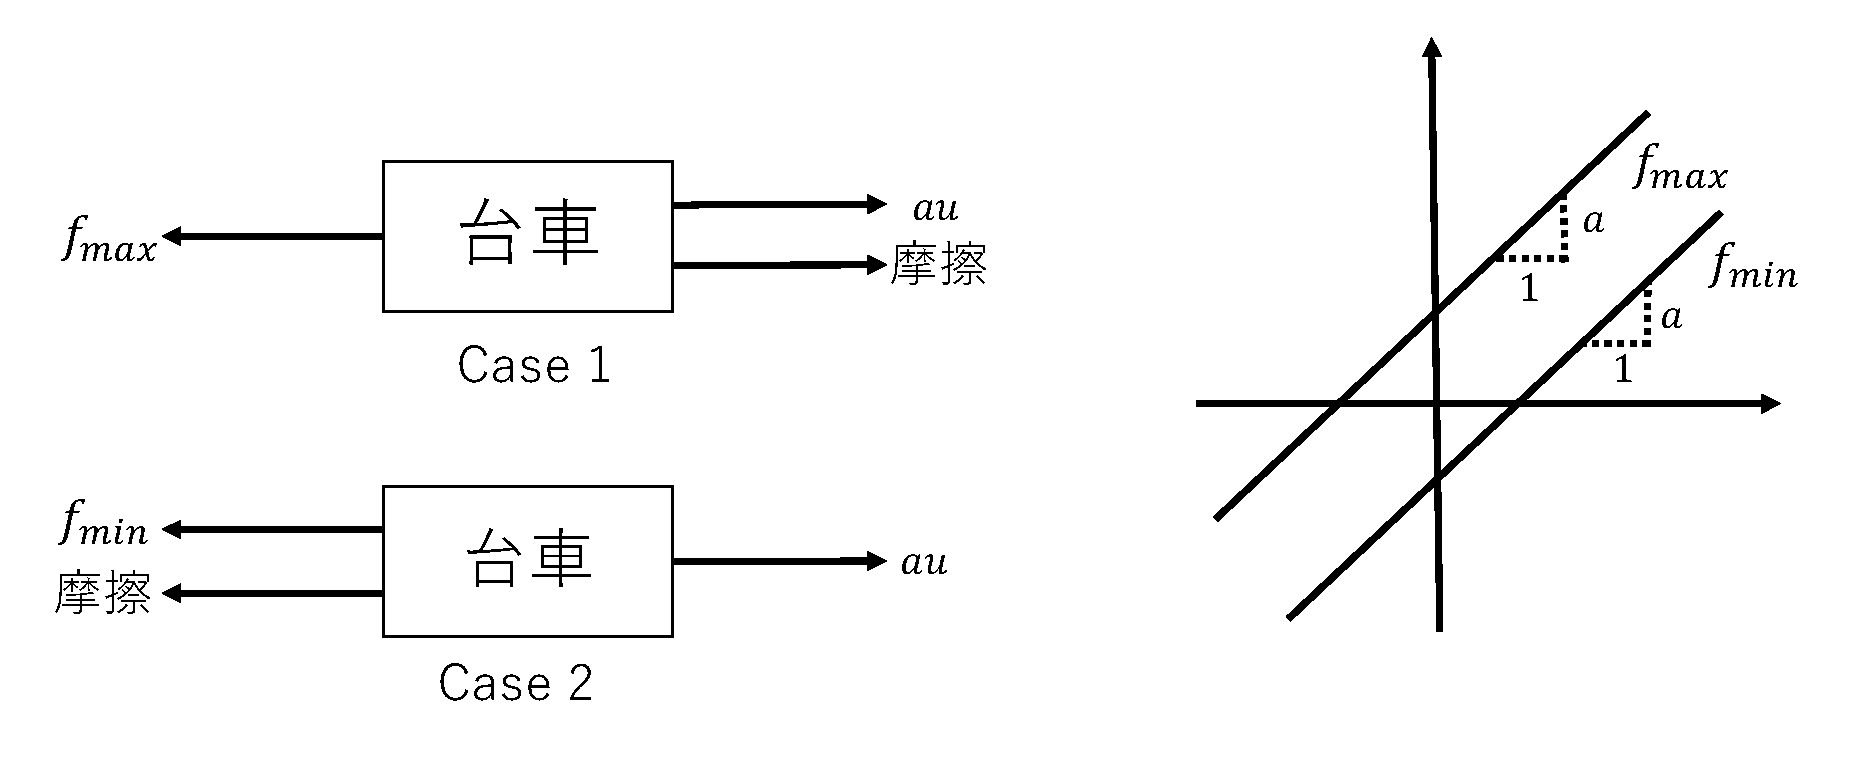
\includegraphics[width=1.0\linewidth]{gazo/ParameterA.eps}
		\caption{パラメータaの決定}
		\label{image:parameterA}
	\end{figure}
	なお、振子は台車から取り外して測定を行う。
	以下に測定した結果から得られた一次関数の傾き$a$を示す。
	\[
		a=0.062[\rm{Kg/V}] = 0.61[\rm{N/V}]
	\]
	
\subsection{Jとcの測定}
	振子を自由振動させることにより、$J$と$c$を測定できる。その数式モデルは鉛直下向きを基準として
	\begin{equation}
		(J + ml^{2})\ddot{\theta} - mgl\sin{\theta} + c\dot{\theta} = 0
		\label{eq:Para1}
	\end{equation}
	\begin{equation}
		y_{2} = c_{2}\theta
	\label{eq:Para2}
	\end{equation}
	で与えられる。$\theta$を微小範囲で考えると、(\ref{eq:Para1}),(\ref{eq:Para2})式は
	\[
		\ddot{y}_{2} + 2\zeta\omega_{n}\dot{y}_{2} + \omega_{n}^{2}y_{2} = 0
	\]
	ただし、
	\[
		\zeta = \frac{c}{2\sqrt{mgl\left(J + ml^{2}\right)}} 
		,\ \  \omega_{n} = \sqrt{\frac{mgl}{J+ml^{2}}}
	\]
	のように書くことができる。この解は
	\[0<\zeta<1\]
	のとき、減衰振動となり
	\[
		y_{2}(t) = \frac{y_{2}(0)}{\sqrt{1-\zeta^{2}}}\exp{(-\omega_{n}\zeta t)}
	  	\sin{(\omega_{n}\sqrt{1-\zeta^{2}}t + \phi)}
	\]
	ただし
	\[
		\phi = \tan^{-1}{\frac{\sqrt{1-\zeta^2}}{\zeta}}
	\]
	で与えられる。\cite{Koga:Binpe}
	\begin{figure}[H]
		\centering
		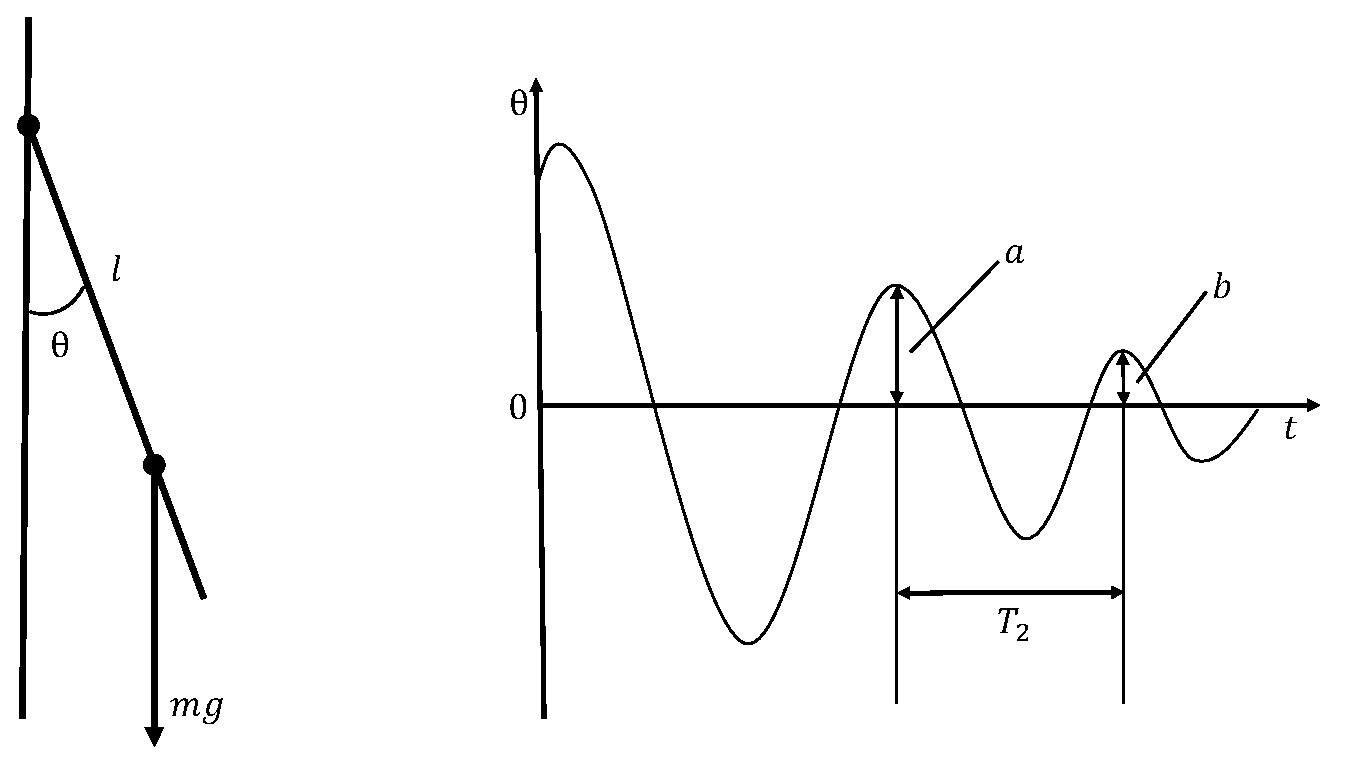
\includegraphics[width=1.0\linewidth]{gazo/ParameterJC.eps}
		\caption{$J$と$c$の測定}
		\label{image:parameterJC}
	\end{figure}
	\par
	いま、減衰振動の周期を$T_{2}$とし、時刻$t_{1}$と時刻$t_{2} = t_{1}+T_{2}$において波形
	$y_{2}(t)$の山が隣合うものとする。このときの振幅の減衰比は
	\[
		\frac{|y_{2}(t_{2})|}{|y_{2}(t_{1})|} = \exp{(-\lambda)}
	\]
	ただし
	\[
		\lambda = \frac{2\pi\zeta}{\omega_{n}\sqrt{1-\zeta^2}} 
	\]
	となる。この$\lambda$は対数減衰比と呼ばれる。また
	\[
		T_{2} = \frac{2\pi}{\omega_{n}\sqrt{1-\zeta^{2}}}
	\]
	が成り立つ。したがって、$J$と$c$は
	\[
		J=\frac{mglT_{2}^{2}}{4\pi^{2}+\lambda^{2}}-ml^{2},\ \ 
		c=\frac{2\lambda(J+ml^{2})}{T_{2}}
	\]
	のように与えられる。\cite{Koga:Binpe}
	以下に振子を自由振動させ得られたデータから計算した$J$と$c$を示す。
	\[
		J=2.5\times10^{-4}[\rm{khm^{2}}]
	\]
	\[
		c=5.4\times10^{-5}[\rm{kgm^{2}/s}]
	\]
	
\subsection{Mとfの測定}
	
	$M$と$f$の測定方法には二通りがある。
	\subsubsection{ステップ応答による測定法}
		ここでは、台車をアンプ・モータプーリ・ベルト・台車系の等価質量と等価摩擦係数とし、
		台車のステップ応答を測定することで$M$と$f$を決定する。
		ただし、振り子は台車から取り外した状態で測定を行う。
		このときの運動方程式は
		\[
			M\ddot{r} = au - f\dot{r}
		\]
		であり、$u$から$r$までの伝達関数$G$は
		\[
			G(s) = \frac{K}{s(Ts+1)}
		\]
		となる。ただし、
		\begin{equation}
			K = \frac{a}{f},\ \ T=\frac{M}{f}
			\label{eq:kt}
		\end{equation}
		である。初期状態を0とするとき、このシステムのステップ応答は
		\begin{equation}
			r(t) = KU_{0}\left(Te^{\frac{-t}{T}}+t-T\right)
			\label{eq:step}
		\end{equation}
		である。
		\begin{figure}[H]
			\centering
			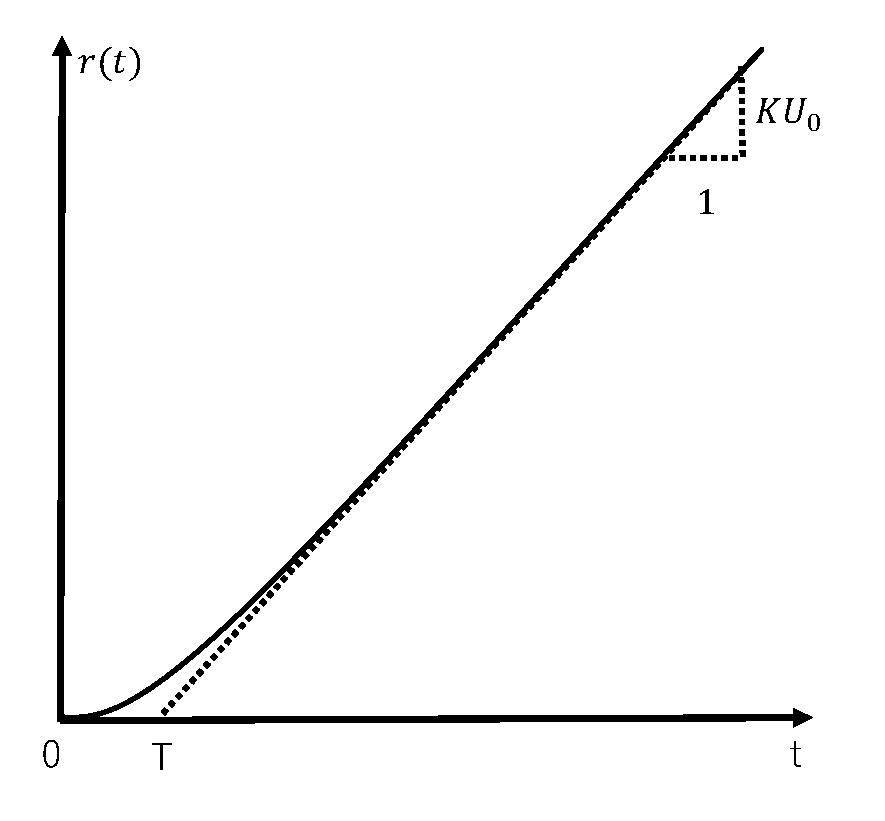
\includegraphics[width=0.6\linewidth]{gazo/step.eps}
			\caption{台車のステップ応答}
			\label{image:parameterMF}
		\end{figure}
		ただし、$U_{0}$はステップの高さである。
		(\ref{eq:step})において$t→\infty$とすれば
		\[
			r(t) = KU_{0}(t-T)
		\]
		となり、図\ref{image:parameterMF}を参考に$T$と$K$をもとめ、
		(\ref{eq:kt})式より$M$と$f$を決定することができる。
		以下にこの方法を用いて同定したパラメータを示す。
		\[
			M=6.9E-1[\rm{kg}]
		\]
		\[
			f=7.6[\rm{kg/s}]
		\]
		
	\subsubsection{フィードバック入力による測定法}
		ここでは、入力にステップ応答ではなく、以下に示すようなフィードバック入力を加える。
		\begin{equation}
			u = k_{c}(y_{c} - y)
		\end{equation}
		ただし、$y_c$は目標値、$y$は出力、$k_{c}$はフィードバックゲインである。
		本節では$k_c=2500$とする。
		このようにすることで不足制動の2次系($\zeta<1$)を実現させる。
		\begin{figure}[H]
			\centering
			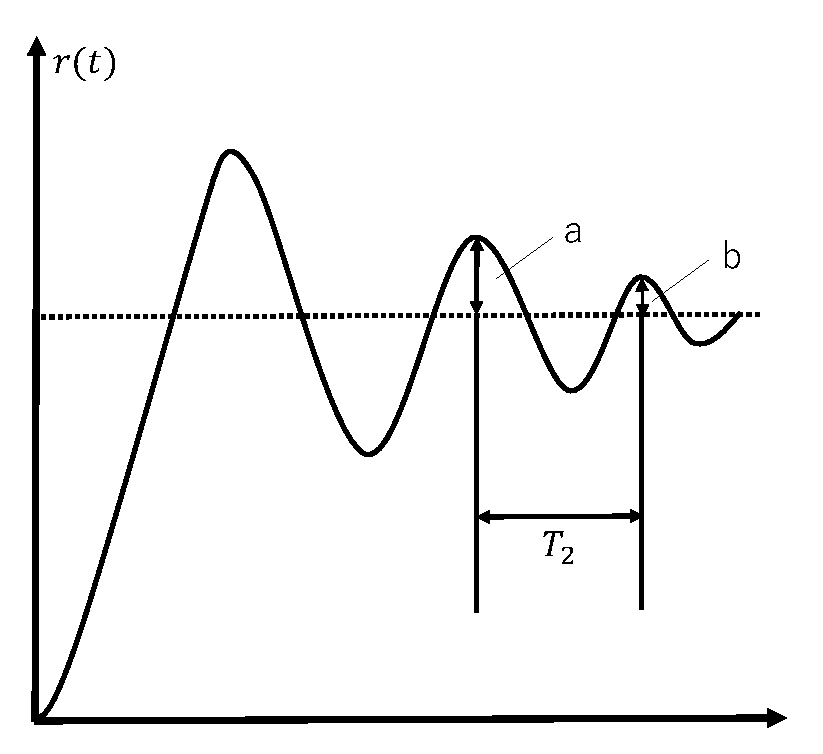
\includegraphics[width=0.6\linewidth]{gazo/feedback.eps}
			\caption{台車のフィードバック応答}
			\label{image:parameterMFfeed}
		\end{figure}
		図\ref{image:parameterMFfeed}を参考にして$M$と$f$を同定する。
		この方法は$J$と$c$の同定の際に用いた方法とほぼ同じであるため、詳しい説明はそちらに
		譲る。
		\par
		台車のフィードバック応答から求めた$\lambda$と$T_2$から以下の式を用いて$\zeta$と$\omega_{n}$を計算し求める。
		\begin{equation}
			\lambda=\frac{2\pi\zeta}{\sqrt{1-\zeta^{2}}}
		\end{equation}
		\begin{equation}
			T_{2}=\frac{2\pi}{\omega_{n}\sqrt{1-\zeta^{2}}}
		\end{equation}
		上の式を式変形して$\zeta$と$\omega_{n}$イコールの式にすると
		\begin{equation}
			\zeta=\frac{\lambda}{\sqrt{4\pi^{2}+\lambda^{2}}}
		\end{equation}
		\begin{equation}
			\omega_{n}=\frac{2\pi}{T_{2}\sqrt{1-\zeta^{2}}}
		\end{equation}
		以上の式から求めた$\zeta$と$\omega_{n}$は以下の二次系の伝達関数の基本形に代入することで
		同定に用いたフィードバック制御系の伝達関数を求めることができる
		\begin{equation}
			G(s) = \frac{\omega_{n}^{2}}{s^{2}+2\zeta\omega_{n}s + \omega_{n}^{2}}
		\end{equation}
		また、今回のフィードバック制御系におけるブロック線図は以下のようになる。
		\begin{figure}[H]
			\centering
			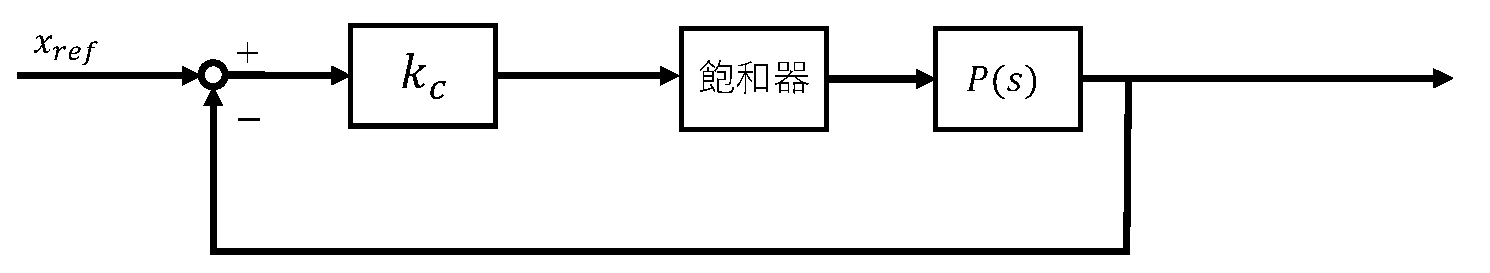
\includegraphics[width=1.0\linewidth]{gazo/FeedBackCart.eps}\\
			\caption{フィードバック制御系のブロック線図}
			\label{image:FeedBackCart}
		\end{figure}
		ここで、$P(s)$は台車の伝達関数であり以下の式で表される。
		\begin{equation}
			P(s)=\frac{K}{s(Ts+1)}
			\label{eq:Ps}
		\end{equation}
		ただし、Tは$M/f$、Kは$a/f$である。上のブロック線図から伝達関数を求める。
		しかし、飽和システムを含んでいると伝達関数を求めることができないので、ここでは飽和システムがなくても
		台車は問題なく動作するものとして仮定する。以上の仮定から伝達関数は
		\begin{equation}
			G(s) = \frac{AK/T}{s^{2}+(1/T)s+(AK/T)}
			\label{eq:Gs}
		\end{equation}
		となる。ただしAはゲインである。(\ref{eq:Ps})式と(\ref{eq:Gs})式を係数比較し、$M,f$イコール
		の式にすると以下のようになる。
		\begin{equation}
			\left.
			\begin{array}{l}
				\displaystyle M=\frac{aA}{\omega_{n}^{2}} , \ f=2\zeta\omega_{n}^{2}M
			\end{array}
			\right.
			\label{eq:mf}
		\end{equation}
		よって、(\ref{eq:mf})式からMとfは以下のように求まる。
		\[
			M=1.59[\rm{kg}]
		\]
		\[
			f=13.2[\rm{kg/s}]
		\]
		
	\subsubsection{$M$と$f$の決定}
	パラメータ$M$と$f$についてはステップ応答による方法とフィードバックによる方法の2通りから
	同定を行った。しかし、それぞれの方法で求めたパラメータを比較するとまるで違うことがわかる。
	これはフィードバックによる方法が十分に正確な方法ではなかったためといえる。
	その原因は、飽和システムを含めずに同定を行ったことではないかと考える。
	シミュレーションにおいては入力にどのような値を加えても倒立振子系に何ら影響はないが
	実際の倒立振子においてはその入力できる値には制限がある。この制限を考えるか否か
	で結果が変わってくるはずである。
	\begin{figure}[H]
		\centering
		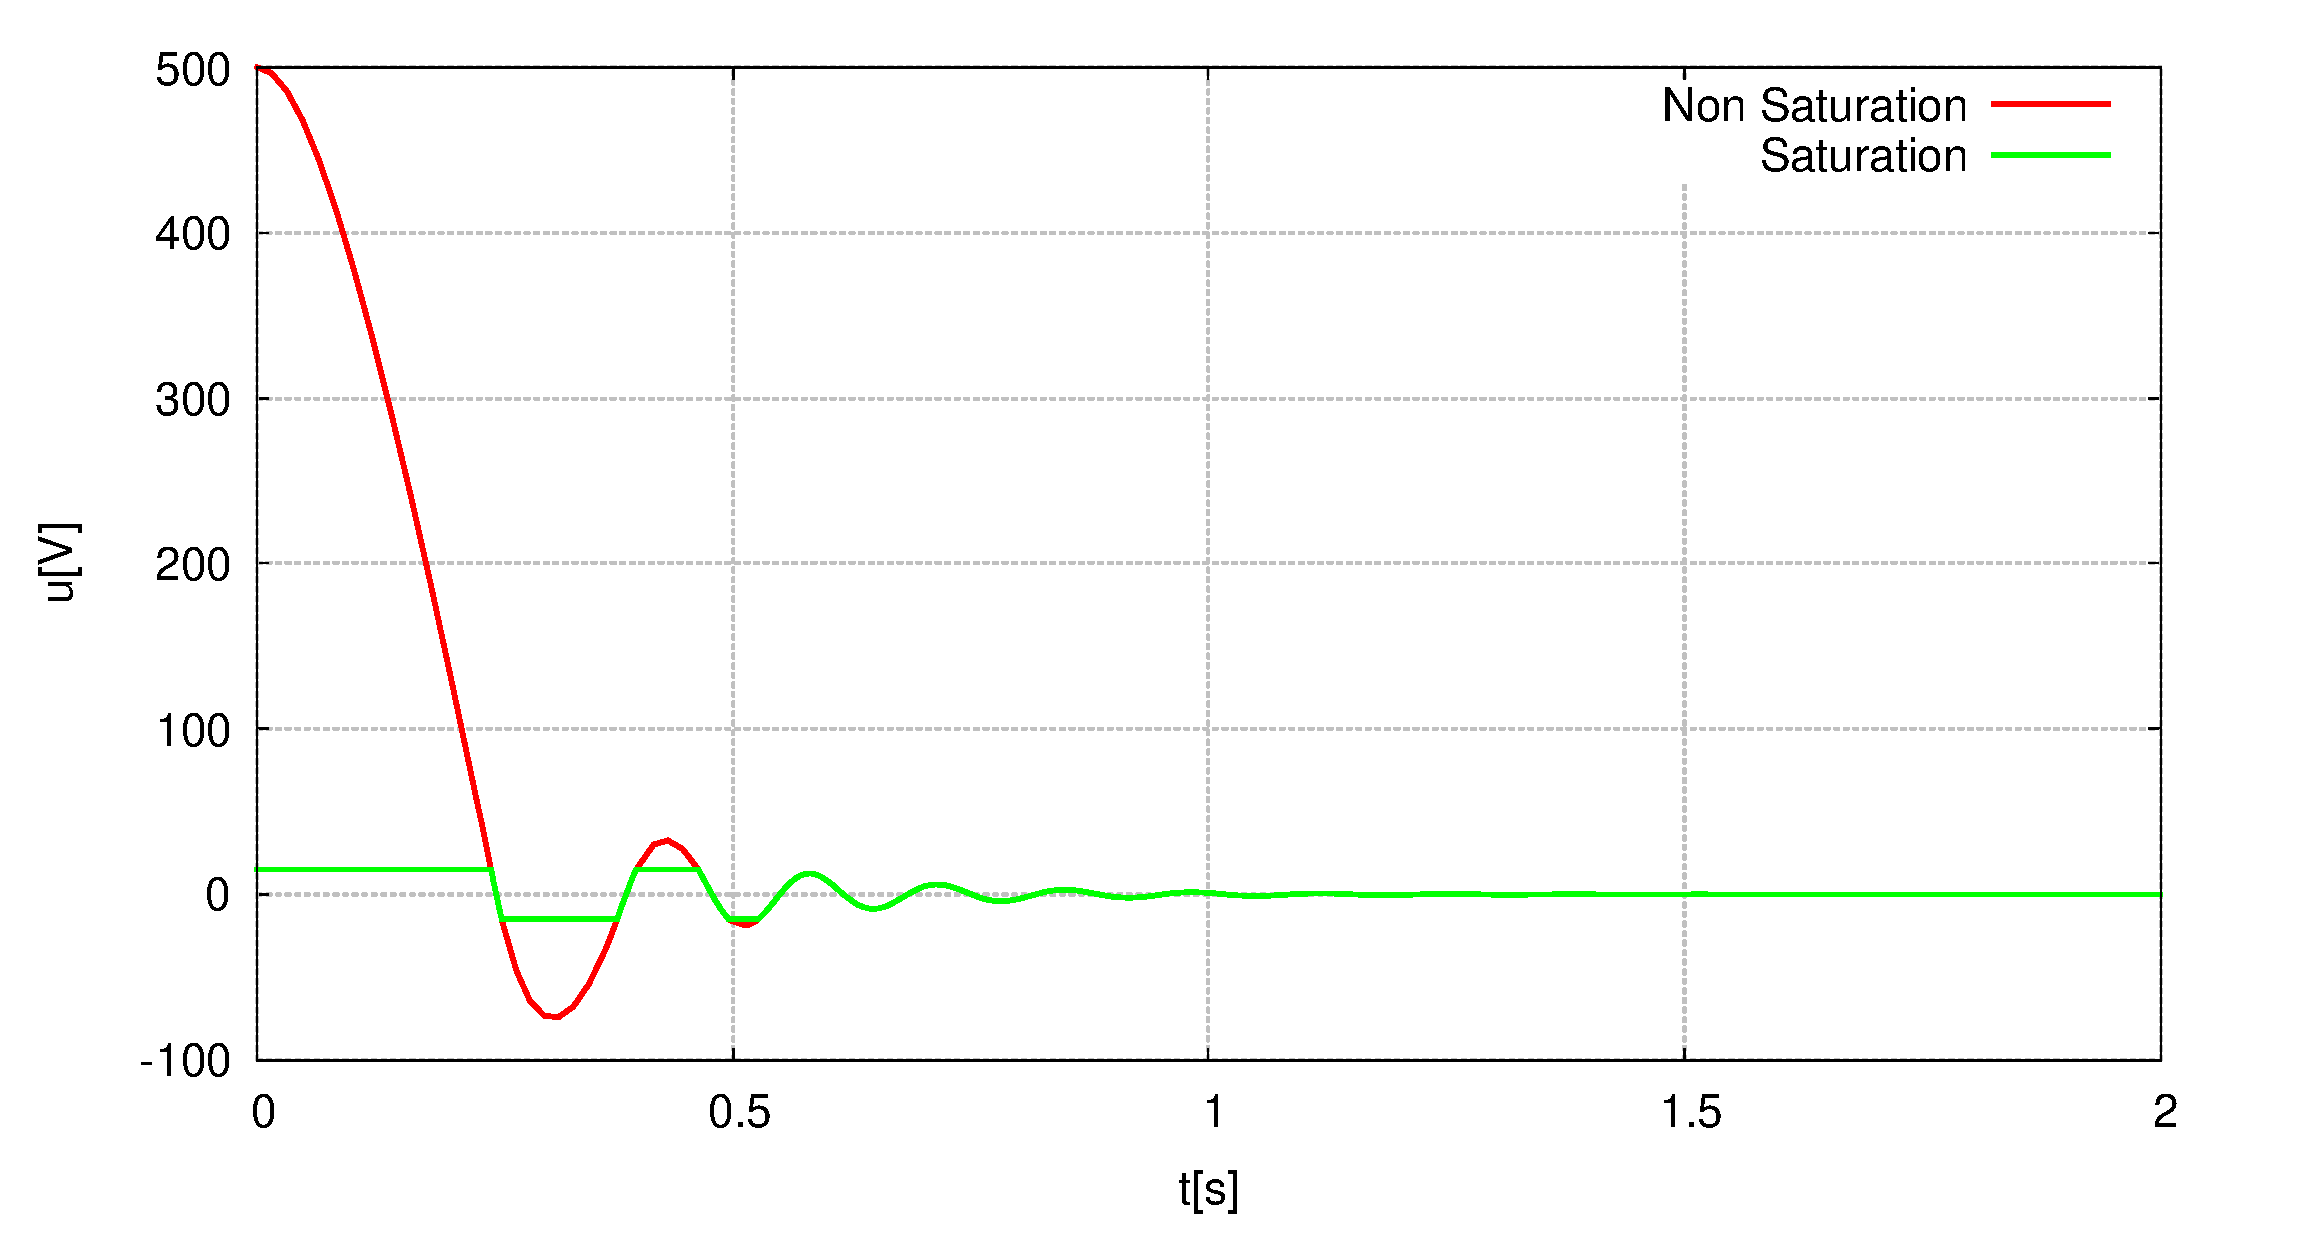
\includegraphics[width=0.8\linewidth]{gazo/feedback_input.eps}\\
		\caption{飽和器の有無によるフィードバック入力の比較}
		\label{image:feedback_saturation}
	\end{figure}
	図\ref{image:feedback_saturation}は図\ref{image:FeedBackCart}のブロック線図において
	飽和器を含めた場合の入力と飽和器を含めなかった場合の入力を描画させたものである。
	この図より、飽和器がない(non Saturation)場合、入力は最大500(V)まで加えられることがわかる。本実験で用いる倒立振子系の入力限界は
	$-15<u<15$であるので、飽和器を加えた場合、その範囲を超える入力は絶対値15(V)に制限されている。
	つまり、フィードバックによる方法で同定したパラメータは飽和器を考慮していないので、現実の倒立振子系とは違うパラメータであるといえる。
	また、今回はフィードバックゲインを2500としたが、
	フィードバックゲインを小さくすると、入力もそれに伴い小さくなるので、
	現実の倒立振子系に近いパラメータを同定することができるはずである。
	以上から本実験においてフィードバックを行う場合、入力が大きく跳ね上がる可能性があるので、必ず飽和システムが必要であるといえる。
	なので、飽和システムが存在する限り伝達関数を求めることができないので、
	正確なパラメータの計算を行うことができないといえる。
	以降、パラメータ$M,f$はステップ応答による方法で同定した値を用いる。
	
\subsection{$c_1$と$c_2$の測定}
	$c_1$と$c_2$に関しては
	\[
		c_1 = 1.0 [\rm{V/m}]
	\]
	\[
		c_2 = 1.0[\rm{V/rad}]
	\]
	というように
	ソフトウェアに設定してあるものを用いた。
\subsection{同定結果}
	同定実験において同定したパラメータを表にまとめる。
	\begin{table}[htb]
		\begin{center}
			\caption{同定したパラメータの一覧}
			\medskip
			
			\begin{tabular}{|l|l|}\hline
				パラメータ & 同定した値 \\ \hline\hline
				m[kg]  & 0.031\\ \hline
				l[m] & 0.15\\ \hline
				M[kg] & 0.69\\ \hline
				f[kg/s] & 7.6\\ \hline
				J[$\rm{kgm}^2$] & $2.5\times10^{-4}$\\ \hline
				c[$\rm{kgm}^2/\rm{s}$] & $5.4\times10^{-5}$\\ \hline
				a[N/V] & 0.61\\ \hline
				$c_{1}$[V/m] & 1.0\\ \hline
				$c_{2}$[V/rad] & 1.0\\ \hline
			\end{tabular}
		\end{center}
	\end{table}
%一次チェック完了:
%-----------------------------------------------------------------------------------------------------	
\section{パラメータの検証}
	前節では、実験によって倒立振子のパラメータを同定した。
	しかし、その同定したパラメータがどれほど有効性があるか現時点では全く分からない状況である。
	そこで、本節では同定したパラメータの有効性をがどれほどなのかシミュレーションを用いて検証を
	行う。シミュレーションに用いたツールはJAMOXである。ただし、直接同定を行った$m,l$や最初から
	設定してあった$c_1,c_2$については検証は行わない。
	\subsection{振子の自由振動シミュレーション}
		ここでは、$J,c$の検証を行う。
		以下にシミュレーションと実験データを描画したグラフを示す。
		\begin{figure}[H]
			\centering
			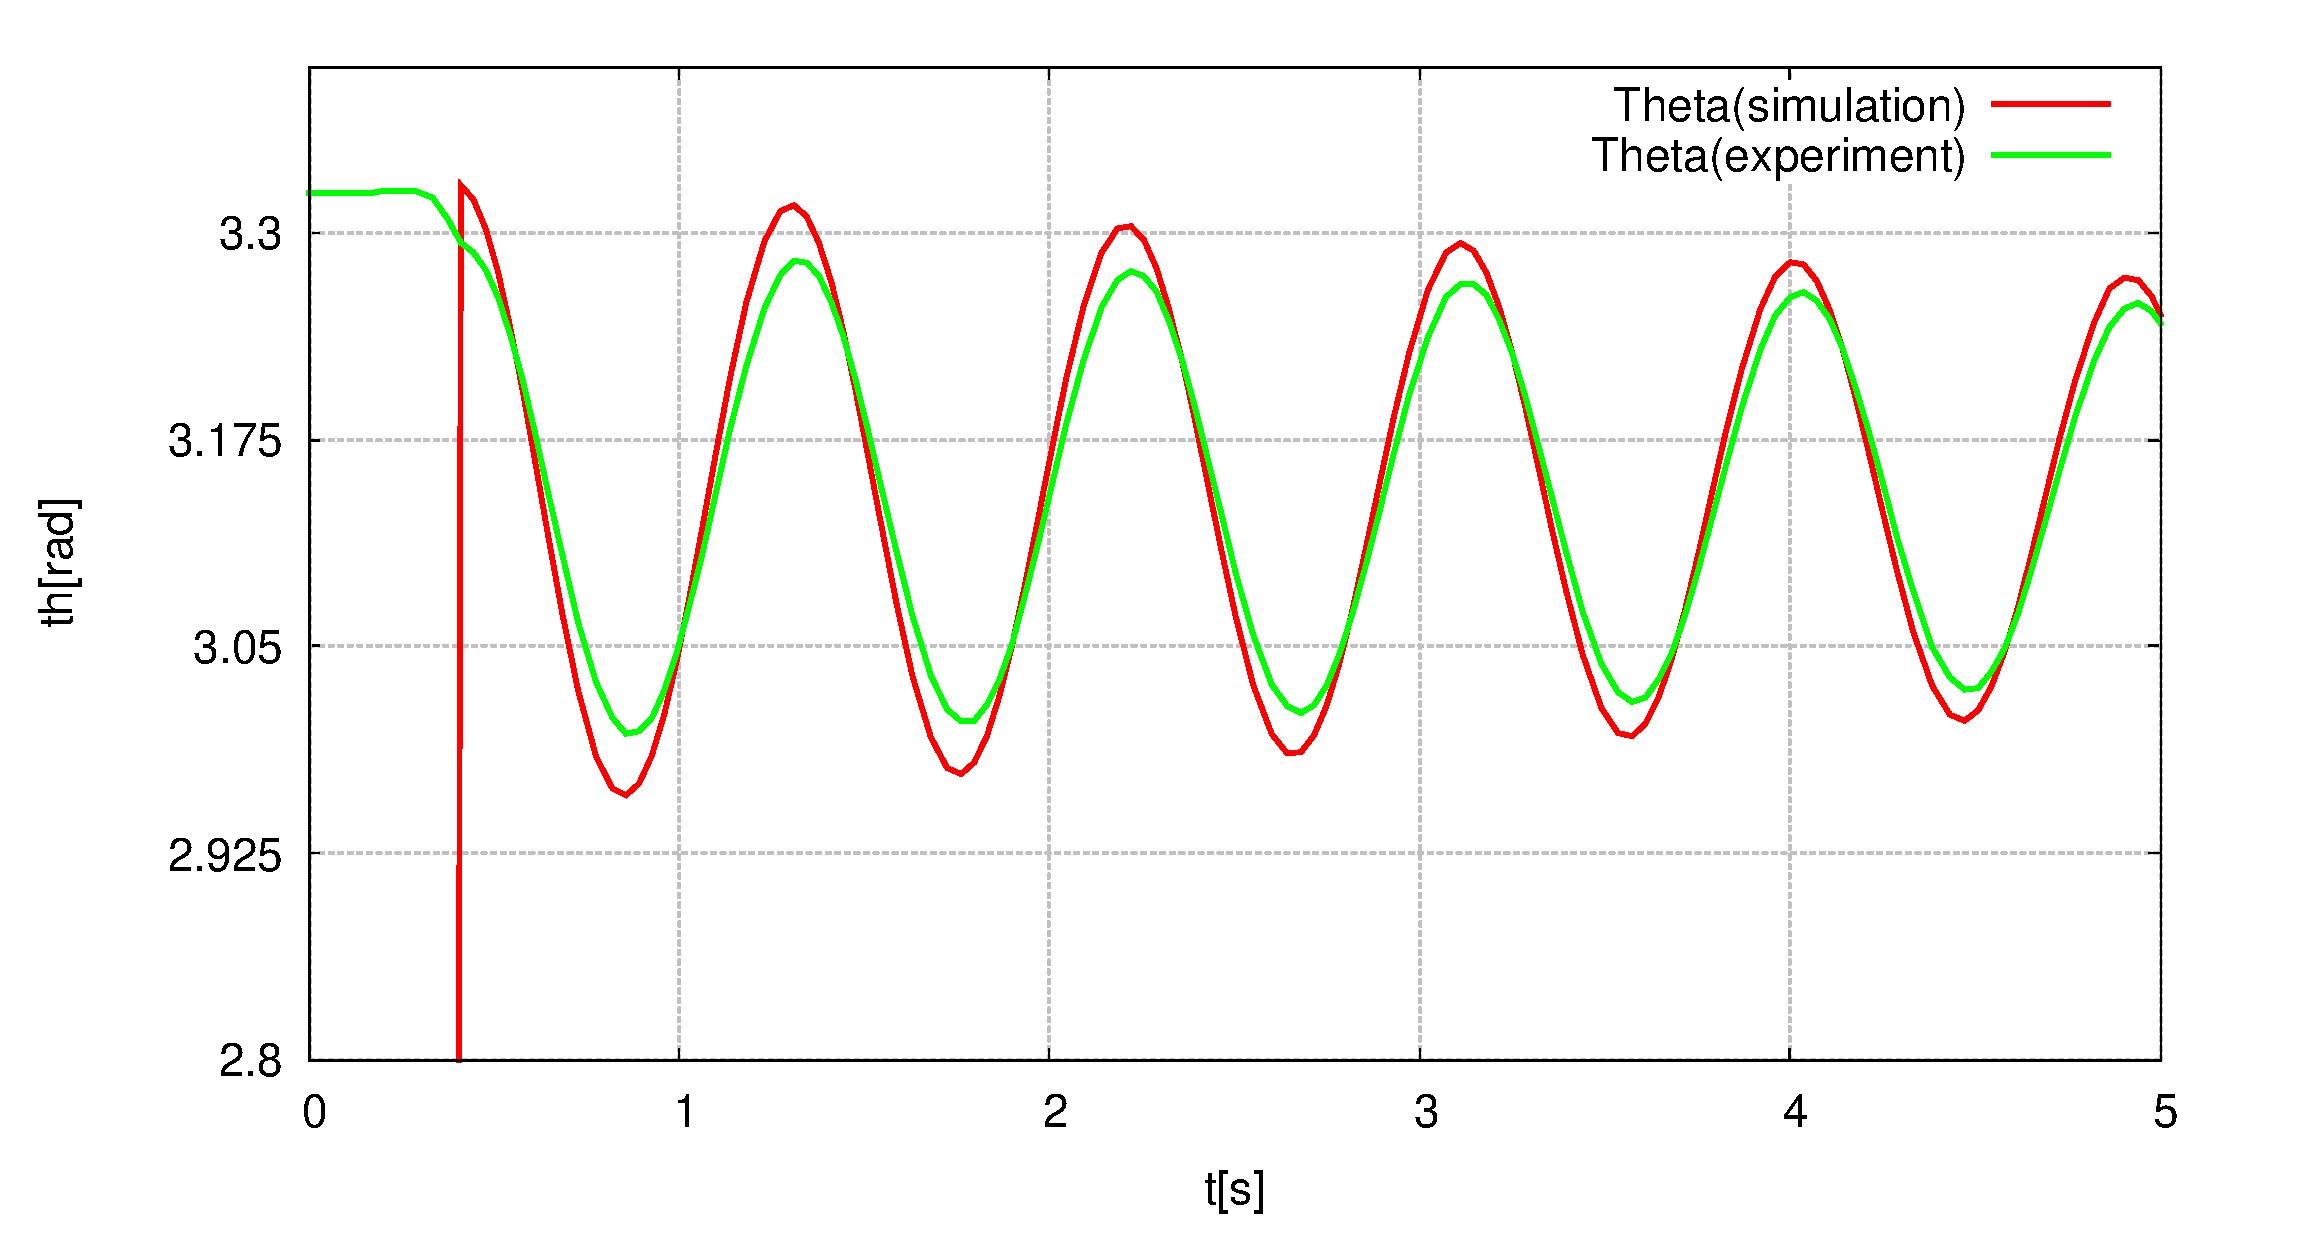
\includegraphics[width=0.8\linewidth]{gazo/free45Auto.eps}\\ 
			\caption{振子の自由振動シミュレーション}
			\label{image:freependulum}
		\end{figure}
		図\ref{image:freependulum}において、シミュレーションは0.32(s)程遅らせて実行しているので、それ以前の時間の角度は$0°$である。
		自由振動の初期角度は$180°$を基準として$10°$である。
		図\ref{image:freependulum}よりシミュレーションと実験結果に少し差異はあるが
		大きな違いはないといえる。よって同定したパラメータ$J,c$は有効な値であるといえる。
		\newpage
	\subsection{台車のステップ応答による方法のシミュレーション}
		ここでは、$M,f,a$の検証を行う。$M,f$はステップ応答による方法で求めた値を用いる。
		以下にシミュレーションと実験データを描画したグラフを示す。
		\begin{figure}[H]
			\centering
			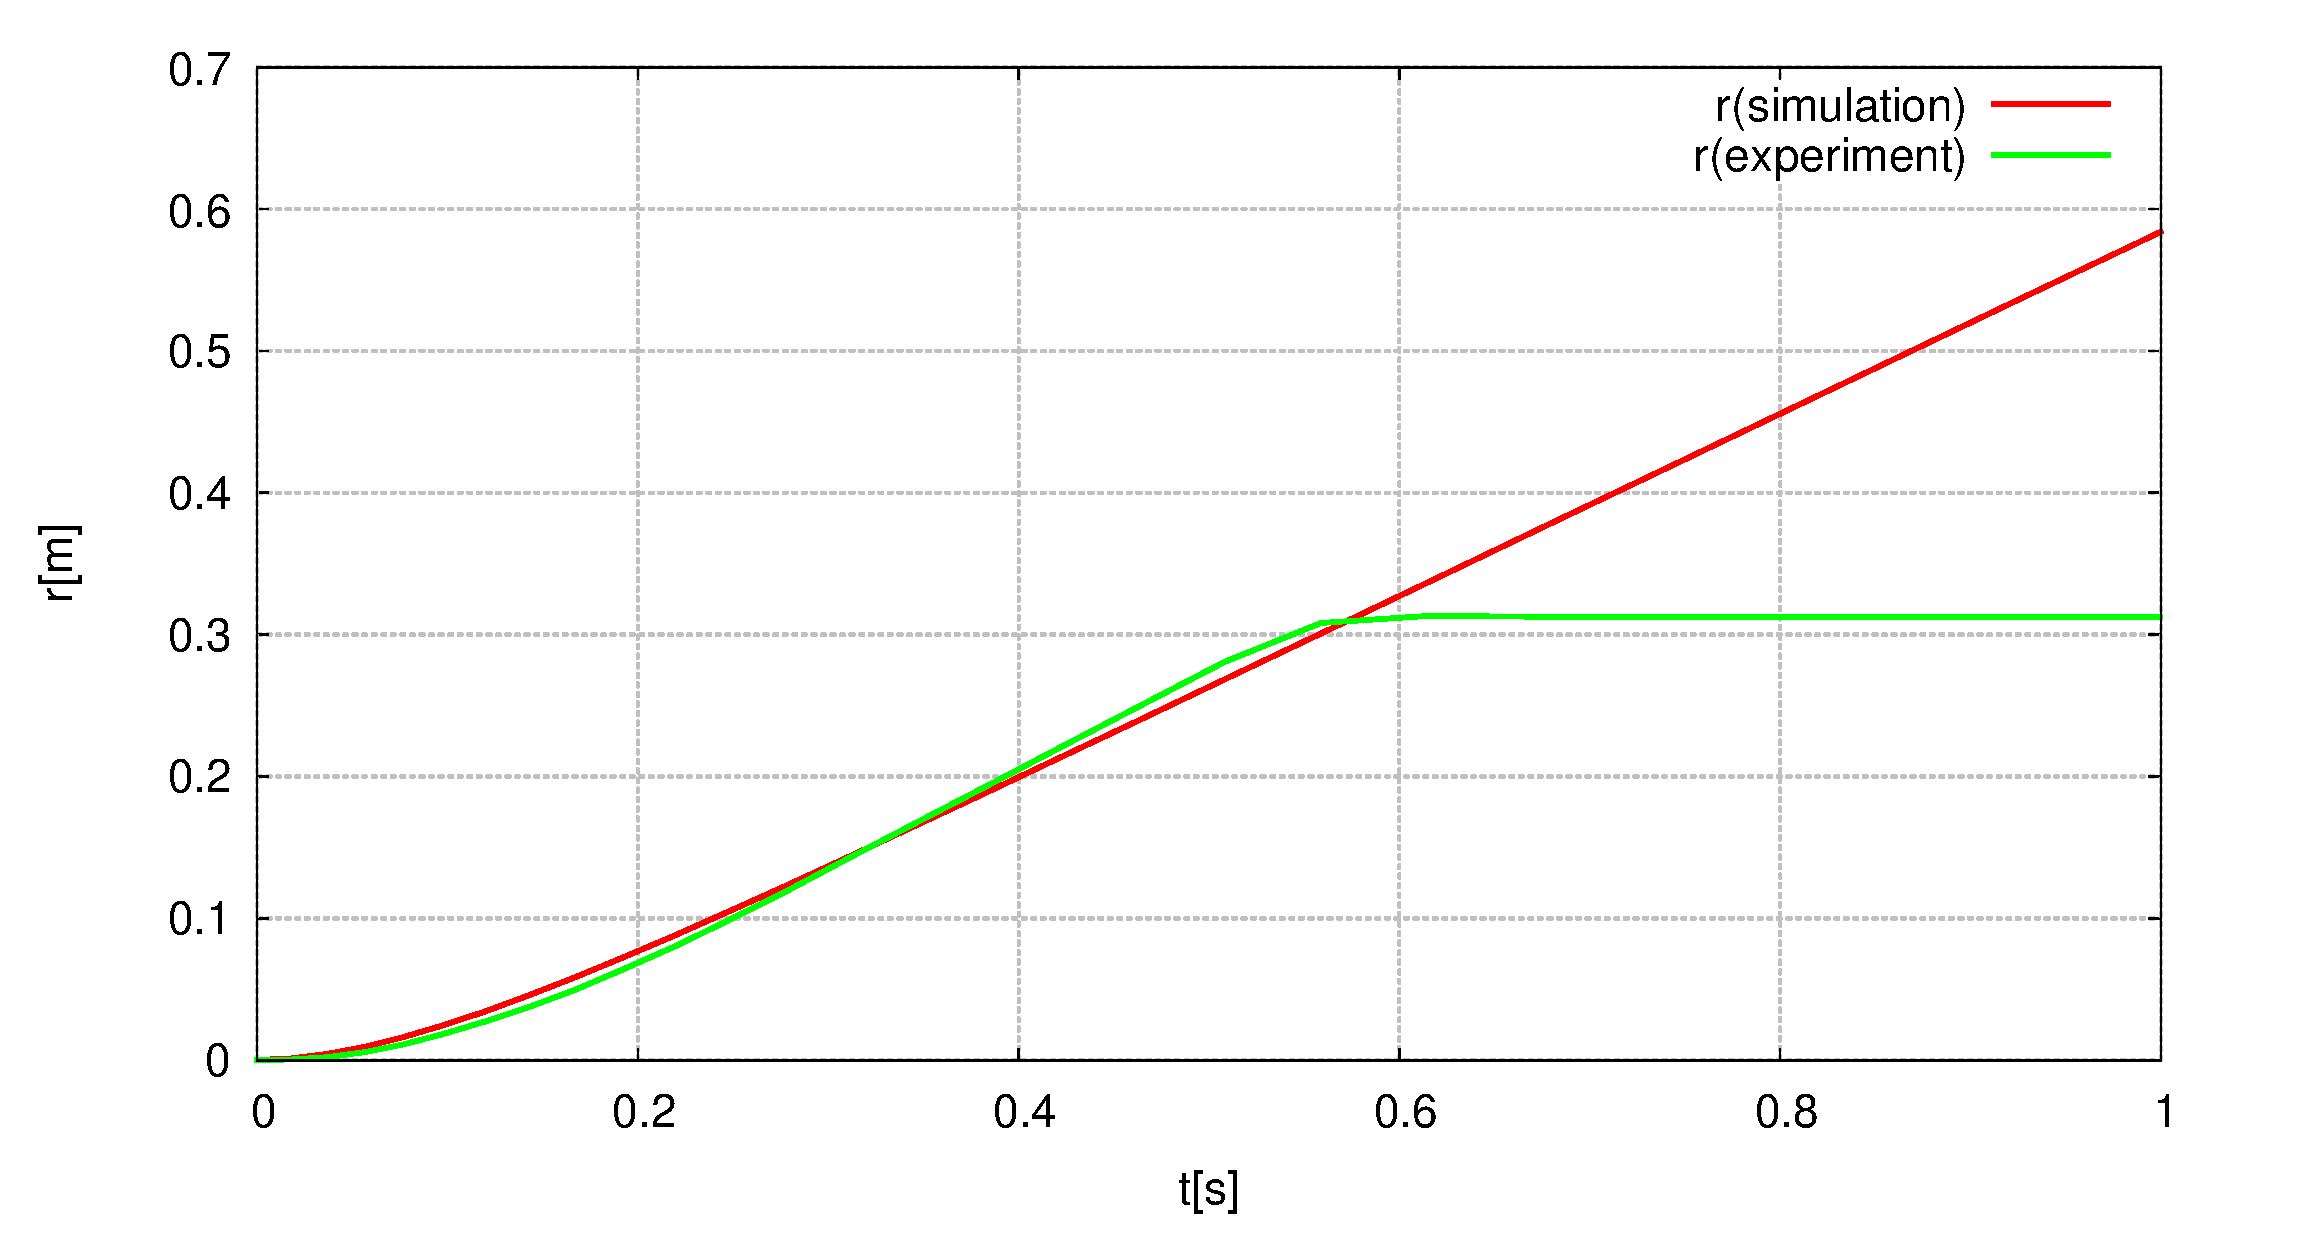
\includegraphics[width=0.8\linewidth]{gazo/nabe8.eps}\\
			\caption{台車のステップ応答シミュレーションと実験結果の比較}
			\label{image:step}
		\end{figure}
		図(\ref{image:step})よりシミュレーションと実験結果に少し差異はあるが
		大きな違いはないといえる。0.6秒以降のグラフが大幅に異なっているが、これはシミュレーションの場合は
		台車の可動範囲に制限がないためずっと台車が移動し続けるが、実験の場合は台車の可動範囲に
		制限があるため、ある時間を境に移動が止まっている。また、このときの入力電圧は$8[\rm{V}]$
		である。以上から同定したパラメータ$M,f,a$は有効な値といえる。
		\newpage
	\subsection{台車のフィードバック応答シミュレーション}
		ここでは、$M,f,a$の検証を行う。$M,f$はフィードバックによる方法で求めた値を用いる。
		%ここの画像はあやしいので差し替え推奨
		以下にシミュレーションと実験データを描画したグラフを示す。ただし、フィードバックゲインは$1500$である。
		\begin{figure}[H]
			\centering
			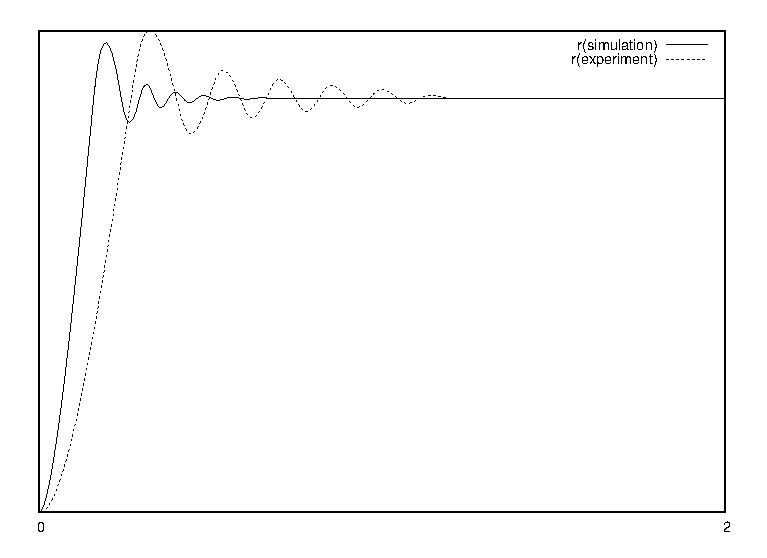
\includegraphics[width=0.8\linewidth]{gazo/feedbackExperiment.eps}
			\caption{フィードバックによる方法のシミュレーションと実験結果の比較}
			\label{image:feedback}
		\end{figure}
		図\ref{image:feedback}よりシミュレーションと実験結果には大きな差異があることが確認できる。
		上述した通りこの方法で同定したパラメータは現実の倒立振子系に即しておらず、結果実験で得られた波形との
		比較において大きな違いが出てきてしまう。よってこの方法で同定したパラメータ$M,f$には
		有効性がないといえる。
		
\section{設計(線形)モデルの決定}
	ここまでで、パラメータを同定し、その有効性についても確かめた。よって、同定すべきパラメータを決定できたので
	システム行列A、入力行列B、出力行列Cを\MaTX{}を用いて計算し、倒立振子の線形モデルを確定する。
	\MaTX{}で計算した各行列を以下に示す。
	\begin{equation}
		A=\left[
		\begin{array}{cccc}
			0 & 0 & 1 & 0 \\
			0 & 0 & 0 & 1 \\
			0 & -0.32 & -10.9 & 0.00038 \\
			0 & 50 & 53 & -0.059 \\
		\end{array}
		\right]
	\end{equation}
	\begin{equation}
		B=\left[
		\begin{array}{c}
			0 \\
			0 \\
			0.87 \\
			-4.3 \\
		\end{array}
		\right]
	\end{equation}
	\begin{equation}
		C=\left[
		\begin{array}{cccc}
			1 & 0 & 0 & 0 \\
			0 & 1 & 0 & 0 \\
		\end{array}
		\right]
	\end{equation}
	ただし、倒立振子を立たせることを目的とするので、上向きを基準としたときの線形状態方程式である。
	%一次チェック完了:
	%---------------------------------------------------------------
\chapter{制御系設計}
	\section{システム解析}
	前章で確定した線形モデルについてシステム解析を行う。これにより今回用いるモデル(上向きを基準とした線形状態方程式)が安定化制御可能か
	判定することができる。具体的には可制御性と可観測性を調べ、それらが存在すれば安定化制御可能であるといえる。
	以下で行う計算はすべて\MaTX{}を用いた。
	\subsection{安定性}
		システムの極($A$の固有値)を計算した結果$D$を以下に示す。
		\begin{equation}
			D=\left[
			\begin{array}{c}
				7.0\\
				0\\
				-6.8\\
				-11\\
			\end{array}
			\right]
			\label{eq:Aeig}
		\end{equation}
		(\ref{eq:Aeig})式より1行目が不安定であり、2行目が安定限界であるので、今回用いるモデルは
		不安定であるといえる。
	\subsection{可制御性}
		可制御性行列は以下のようになる。
		\[
			N_{c} = \left[
			\begin{array}{cccc}
				C & CA & CA^{2} & CA^{3} \\
			\end{array}
			\right]
		\]
		上の行列よりランクは4になれば可制御性があるといえる。ランクを計算したところ
		\[
			\rm{rank}  = 4
		\]
		となった。よって可制御性を確認できる。\\
	\subsection{可制御性}
		可観測性行列は以下のようになる。
		\[
			N_{o} = \left[
			\begin{array}{c}
				C\\
				CA\\
				CA^{2}\\
				CA^{3}\\
			\end{array}
			\right]
		\]
		上の行列よりランクは4になれば可観測性があるといえる。ランクを計算したところ
		\[
			\rm{rank} = 4
		\]
		となった。よって、可観測性を確認できる。\\
	\par
	以上から倒立振子系の上向き基準の線形モデルは不安定なシステムであるが、4つの状態を観測することができ、
	制御することが可能なシステムといえる。次の節では倒立振子を立たせるための制御器を設計していく。
	その際に前章で計算したシステム行列Aと入力行列Bを用いる。
		
%----------------------------------------------------------------------------------
\section{状態フィードバックの設計}
	制御器を設計していく第一段階として、状態フィードバック$F$の設計を行う。
	$F$は、システムを安定化する状態フィードバック
	\[
		u = -Fx
	\]
	として求めればよい。
	また、本実験においては台車が目標値へ移動を行うので、目標値$x_{ref}$
	として以下を設計することになる。
	\begin{equation}
		u(t) = F(x_{ref} - x)
		\label{eq:Feq1}
	\end{equation}
	% TODO←???
	この状態フィードバックの設計法には、極配置に基づく状態フィードバック測と
	LQ最適制御に基づく状態フィードバック測の2通りがあるが今回は後者の方法を用いて設計を行う。
	\par
	さて、(\ref{eq:Feq1})式をLQ問題の解として得るために、2次形式評価関数
	\begin{equation}
		J = \int_{0}^{\infty}(x^{T}Qx+Ru^{2})dt
		\label{eq:Feq2}
	\end{equation}
	\begin{equation}
		Q = \rm{diag}(q_{1}^2,q_{2}^2,q_{3}^2,q_{4}^2),\ \ R = 1
		\label{eq:Feq3}
	\end{equation}
	を考える。ただし、 $\rm{diag}(\ldots)$は、対角行列を表す。これは
	\begin{equation}
		J=\int_{0}^{\infty}(q_{1}^{2}r^{2}+q_{2}^{2}\theta^{2}
		+q_{3}^{2}\dot{r}^{2}+q_{4}^{2}\dot{\theta}^{2})dt
	\end{equation}
	のように表されることから、$q_1,q_2,q_3,q_4$は台車位置$r$、振り子角度$\theta$、
	台車速度$\dot{\theta}$、振子角速度$\dot{\theta}$の間のバランスをとる重み係数である。
	\par
	(\ref{eq:Feq2})と(\ref{eq:Feq3})式を最小にする(\ref{eq:Feq1})式における$F$は、
	リカッチの方程式
	\[
		A^{T}P+PA-PBR^{-1}B^{T}P+Q = 0
	\]
	の解$P>0$を求めて
	\[
		F = R^{-1}B^{T}P
	\]
	のように与えられる。
	\begin{figure}[h]
		\centering
		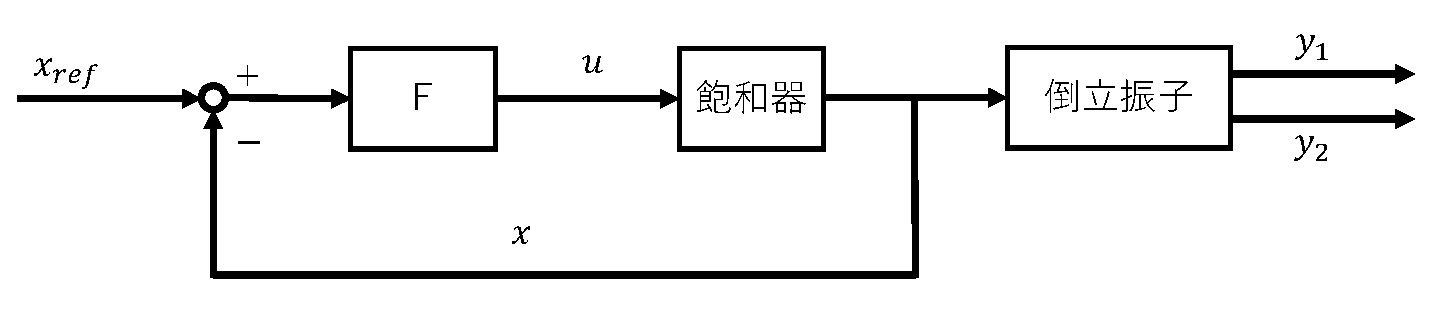
\includegraphics[width=0.8\linewidth]{gazo/controll_F.eps}
		\caption{状態フィードバックを含めたブロック線図}
		\label{image:cF}
	\end{figure}
%一次チェック完了
%----------------------------------------------------------------------------------
\section{最小次元オブザーバの設計}
	第二段階として、
	\begin{equation}
		\hat{x}→x\ \ (t→\infty)
		\label{eq:obs1}
	\end{equation}
	を満足させる状態を推定する状態観測器(最小次元オブザーバ)
	\begin{equation}
		\dot{z}(t) = \hat{A}z(t)+\hat{B}y(t)+\hat{J}u(t)
		\label{eq:obs2}
	\end{equation}
	\begin{equation}
		\hat{x}(t) = \hat{C}z(t) + \hat{D}y(t)
		\label{eq:obs3}
	\end{equation}
	をゴピナスの方法で設計する。
	この方法は、ある行列$U(1×4)$が存在して
	\[
		\begin{array}{c}
			UA = \hat{A}U + \hat{B}C \\
			UB = \hat{J}
			I = \hat{C}U + \hat{D}C
		\end{array}
	\]
	かつ$\hat{A}$が安定行列であることを満足する方法であり、オブザーバ(\ref{eq:obs2})、(\ref{eq:obs3})
	が(\ref{eq:obs1})式を満足するための十分条件でもある。
	なお、本実験で用いる倒立振子系は
	$r,\theta$はセンサーを用いて計測できるが、$\dot{r},\dot{\theta}$
	においては計測するためのセンサーが存在しないため、推測でしかこれらを得ることができない。
	その推測を行うのに、最小次元オブザーバーを用いる。
	\par
	具体的には、オブザーバの係数行列$\hat{A},\hat{B},\hat{J},\hat{C},\hat{D}$を求める。これらは適当な
	オブザーバの極を選択することで得ることができる。。
	また、オブザーバの極を決める際に、状態フィードバック制御
	\[
		u(t) = F(x_{ref}(t)-x(t))
	\]
	による閉ループ系
	\[
		\dot{x}(t) = (A-BF)x(t) + BFx_{ref}(t)
	\]
	の極との位置関係を考慮する必要がある。
	\begin{figure}[h]
		\centering
		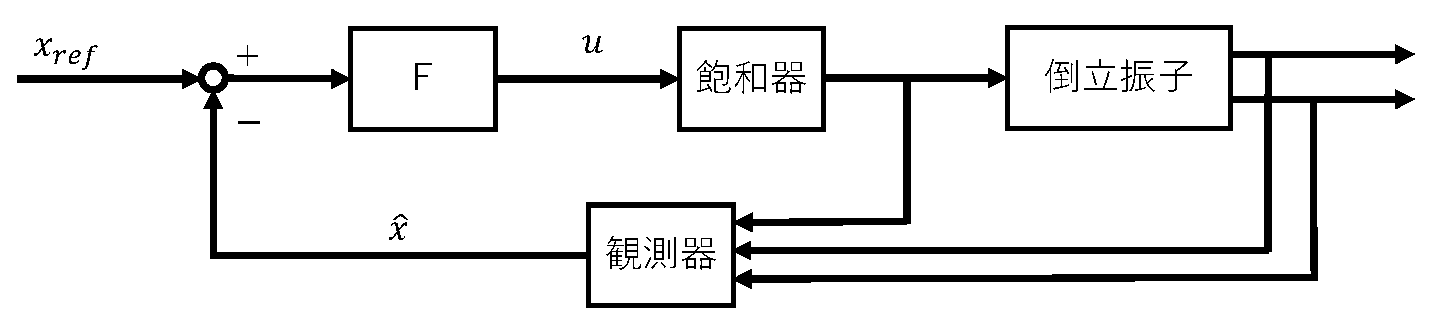
\includegraphics[width=0.8\linewidth]{gazo/controll_obs.eps}
		\caption{最小次元オブザーバーを含めたブロック線図}
		\label{image:cOBS}
	\end{figure}
%一次チェック完了
%----------------------------------------------------------------------------------
\section{コントローラの離散化}
	コントローラは連続時間で記述された(\ref{eq:Feq1})、(\ref{eq:obs2})、(\ref{eq:obs3})式
	で与えられるが、計算機制御のためにはこれらを離散時間で記述しなければならない。
	これらを離散化したものを離散時間コントローラと呼ぶ。離散時間コントローラは
	サンプリング周期を$\Delta$とすると、以下の式で与えられる。
	\begin{equation}
		z[k+1] = \hat{A}_{d}z[k]+\hat{B}_{d}y[k]+\hat{J}_{d}u[k]
	\end{equation}
	\begin{equation}
		\hat{x}[k] = \hat{C}_{d}z[k] + \hat{D}_{d}y[k]
	\end{equation}
	\begin{equation}
		u[k] = F(x_{ref}[k] - \hat{x}[k])
	\end{equation}
	ただし、$k = 0,1\ldots$であり
	\[
		\left(
		\begin{array}{cc}
			\hat{A}_{d} & [\hat{B}_{d}\ \hat{J}_{d}]\\
			0_{3×2} & I_{3}\\
		\end{array}
		\right)=\exp\left(\Delta\left(
		\begin{array}{cc}
			\hat{A} & [\hat{B}\ \hat{J}]\\
			0_{3×2} & I_{3}\\
		\end{array}
		\right)\right)
	\]
	である。
	具体的には、適当なサンプリング周期を$\Delta$を設定すればよい。
	\begin{figure}[h]
		\centering
		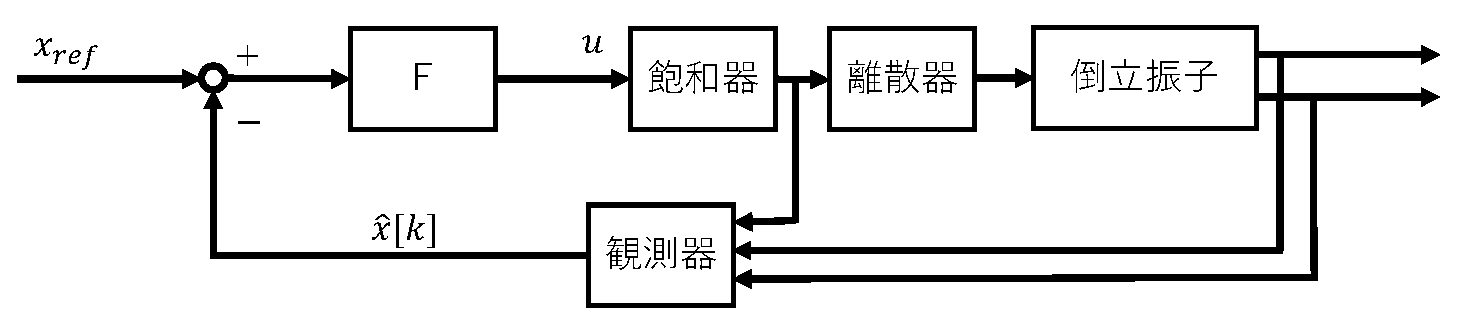
\includegraphics[width=0.8\linewidth]{gazo/controll_discrete.eps}
		\caption{離散器(0次ホールド)を含めたブロック線図}
		\label{image:cDISCRETE}
	\end{figure}
%一次チェック完了
%----------------------------------------------------------------------------------
\section{振り上げ制御及び安定化の実現}
	ここでは振子の振り上げ制御を行うためのコントローラを設計する。振り上げ制御とは、
	振り子を下向きにしたままで台車を動かすことで振り子を倒立させようという制御のことである。
	この制御には振り子を振り上げる制御と振り子の安定化制御を使い分けることで実現させる。
	具体的には下向きの振り子を振り上げ制御により徐々に上に持っていく($\theta$を0に近づけていく)、
	このときある一定の角度を境界値と定め、その境界値まで振り子の角度がちいさくなったところで制御を
	安定化制御に切り替え、安定化制御を行うというものである。振り子の安定化制御についてはこれまでのコントローラを用いるので、
	ここでは振り子の振り上げ制御の理論とその実現方法について述べる。
	\par
	台車と振り子の運動方程式は
	\begin{equation}
		(M+m)\ddot{r}+ml\cos{\theta}\ddot{\theta} = -f\dot{r} + ml\sin{\theta}\dot{\theta}^{2}+au\\
		\label{eq:huriage2}
	\end{equation}
	\begin{equation}
		ml\cos{\theta}\ddot{r}+(J+ml^{2})\ddot{\theta} = mgl\sin{\theta}-c\dot{\theta}\\
		\label{eq:huriage5}
	\end{equation}
	で与えられる。振り子が垂直上向きのときを基準とする振り子の力学的エネルギーは
	\[
		E = \frac{1}{2}(J+ml^{2})\dot{\theta}^{2}+mgl(\cos{\theta}-1)
	\]
	で与えられる。第一項が回転に関するエネルギーであり、第二項が傾きを考慮した位置エネルギーである。
	なお、基準において静止しているとき、力学的エネルギーはE=0である。
	このとき、力学的エネルギーの時間微分は
	\begin{equation}
		\frac{dE}{dt} = (J+ml)\dot{\theta}\ddot{\theta}-mgl\dot{\theta}\sin{\theta}
		\label{eq:huriage6}
	\end{equation}
	となる。振り上げ制御のために、次の制御則を用いる。
	\begin{equation}
		u = \frac{1}{a}\left(f\dot{r} - ml\sin{\theta}\dot{\theta}^{2} + ml\cos{\theta}\ddot{\theta} + (M+m)v \right)\\
		\label{eq:huriage1}
	\end{equation}
	\begin{equation}
		v = -\frac{c\dot{\theta}}{ml\cos{\theta}}+k(E-E_{0})\rm{sign}(\dot{\theta}\cos{\theta})
		\label{eq:huriage4}
	\end{equation}
	ただし、signは符合関数であり、引数の値が負のとき$-1$、正のとき1、0のとき0となる。
	(\ref{eq:huriage1})式を(\ref{eq:huriage2})式に代入すると、
	\begin{equation}
		\ddot{r} = v
		\label{eq:huriage3}
	\end{equation}
	を得る。(\ref{eq:huriage3})式と(\ref{eq:huriage4})式を(\ref{eq:huriage5})式に代入すると
	\[
		(J+ml^{2})\ddot{\theta} = mgl\sin{\theta}-ml\cos{\theta}(k(E-E_{0})\rm{sign}(\dot{\theta}\cos{\theta})
	\]
	を得る。この式を(\ref{eq:huriage6})式に代入すると
	\begin{align*}
			\displaystyle\frac{dE}{dt} &= -ml\dot{\theta}(k(E-E_{0})\rm{sign}(\dot{\theta}\cos{\theta})) \notag\\
			&= -mlk(E-E_{0})\rm{sign}(\dot{\theta}\cos{\theta})(\dot{\theta}\cos{\theta})
	\end{align*}
	となる。リアプノフ関数の候補として、
	\[
		V = \frac{(E-E_{0})^{2}}{2}≧0
	\]
	を考える。Vの時間微分を求めると、
	\begin{align*}
			\displaystyle \frac{dV}{dt} &= (E - E_{0})\frac{dE}{dt} \notag \\
			&= -mlk(E-E_{0})^{2}\rm{sign}(\dot{\theta}\cos{\theta})(\dot{\theta}\cos{\theta})≦0
	\end{align*}
	これより、$\dot{\theta}\cos{\theta}≠0$のとき、$\dot{V}<0$であるので$V$は減少して$0$に収束し、
	$E$は$E_0$に収束する。なお、$k$を大きくすると、早く$E$が$E_0$に収束する。
	実際の制御では、台車の加速度目標vを制限し、
	\begin{align}
			u &= \displaystyle\frac{1}{a}\left(f\dot{r} - ml\sin{\theta}\dot{\theta}^2 + ml\cos{\theta}\ddot{\theta}+(M+m)v \right) \notag\\
			v &= -\displaystyle\frac{c\dot{\theta}}{ml\cos{\theta}}+\rm{sat}_{ng}(k(E-E_{0})\rm{sign}(\dot{\theta}\cos{\theta}) \notag
	\end{align}
	とする。ただし、satは最小値が$-ng$,最大値が$ng$の飽和関数である。$n$は、重力加速度(鉛直下向き)
	と台車の加速度(水平方向)の比である。\\
	具体的には、$k$と重力加速度と台車の加速度の比である$n$を調整し、振り上げ制御を実現させる。
	\begin{figure}[H]
		\centering
		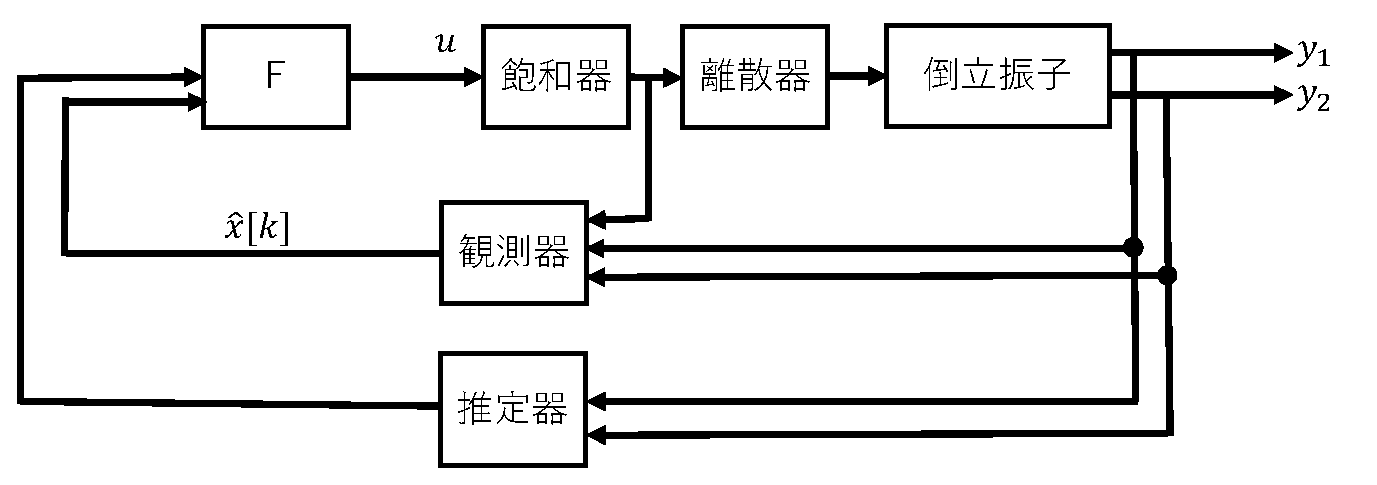
\includegraphics[width=0.8\linewidth]{gazo/controll_huriage.eps}
		\caption{振り上げ制御及び安定化制御を行うためのブロック線図}
		\label{image:cHURIAGE}
	\end{figure}
%一次チェック完了
%----------------------------------------------------------------------------------
\chapter{シミュレーション}
	目標値変更のシミュレーションによって制御器に関する各パラメータの有効な値を探索する。 シミュレーションにはJAMOXを用いた。
% --------------------------------------------------------------------------------------
\section{重み行列の変更による制御性能評価}
	LQ最適制御に基づく状態フィードバック$F$を設計するために
	連続時間線形二次レギュレーターを用いる。この時、連続時間線形二次レギュレーターには
	システム行列$A$と入力行列$B$と重み行列$Q,R$が必要である。
	重み行列は、(\ref{eq:Feq1})式で与え、この重み行列を
	調整することで倒立振子の安定化制御の性能を高めることができる。
	そこで、シミュレーションを用いて重み行列を変更させたときの制御性能について考察していく。
	\par
	今回は行列$R$の値は変更しないので、行列$Q$のみ値を変更してシミュレーション結果を考察する。
	便宜上、重み行列$Q$の対角成分を左から第1成分、第2成分、第3成分、第4成分と呼ぶことにする。
	以下にシミュレーションを行う異なるパターンのパラメータをまとめた表とその時のシミュレーション結果を示す。
	\begin{table}[htb]
		\begin{center}
			\caption{重み行列の変更パターン}
			%\medskip
			\begin{tabular}{|c|c|c|c|}\hline
				& 重み行列$Q$ & オブザーバの極$P$ & サンプリング周期$\Delta[\rm{s}]$ \\ \hline\hline
				パターン1 & $Q_1$:$\rm{diag}(1E5,1E5,1,1)$ & $P_1$:$((-60,0),(-60,0))^{'}$ & $\Delta_1$:0.005 \\ \hline
				パターン2 & $Q_2$:$\rm{diag}(1E6,1E5,1,1)$ & $P_1$:$((-60,0),(-60,0))^{'}$ & $\Delta_1$:0.005 \\ \hline
				パターン3 & $Q_3$:$\rm{diag}(1E5,1E6,1,1)$ & $P_1$:$((-60,0),(-60,0))^{'}$ & $\Delta_1$:0.005 \\ \hline
			\end{tabular}
		\end{center}
		\label{table:QRF}
	\end{table}
	
	\begin{figure}[H]
		\centering
		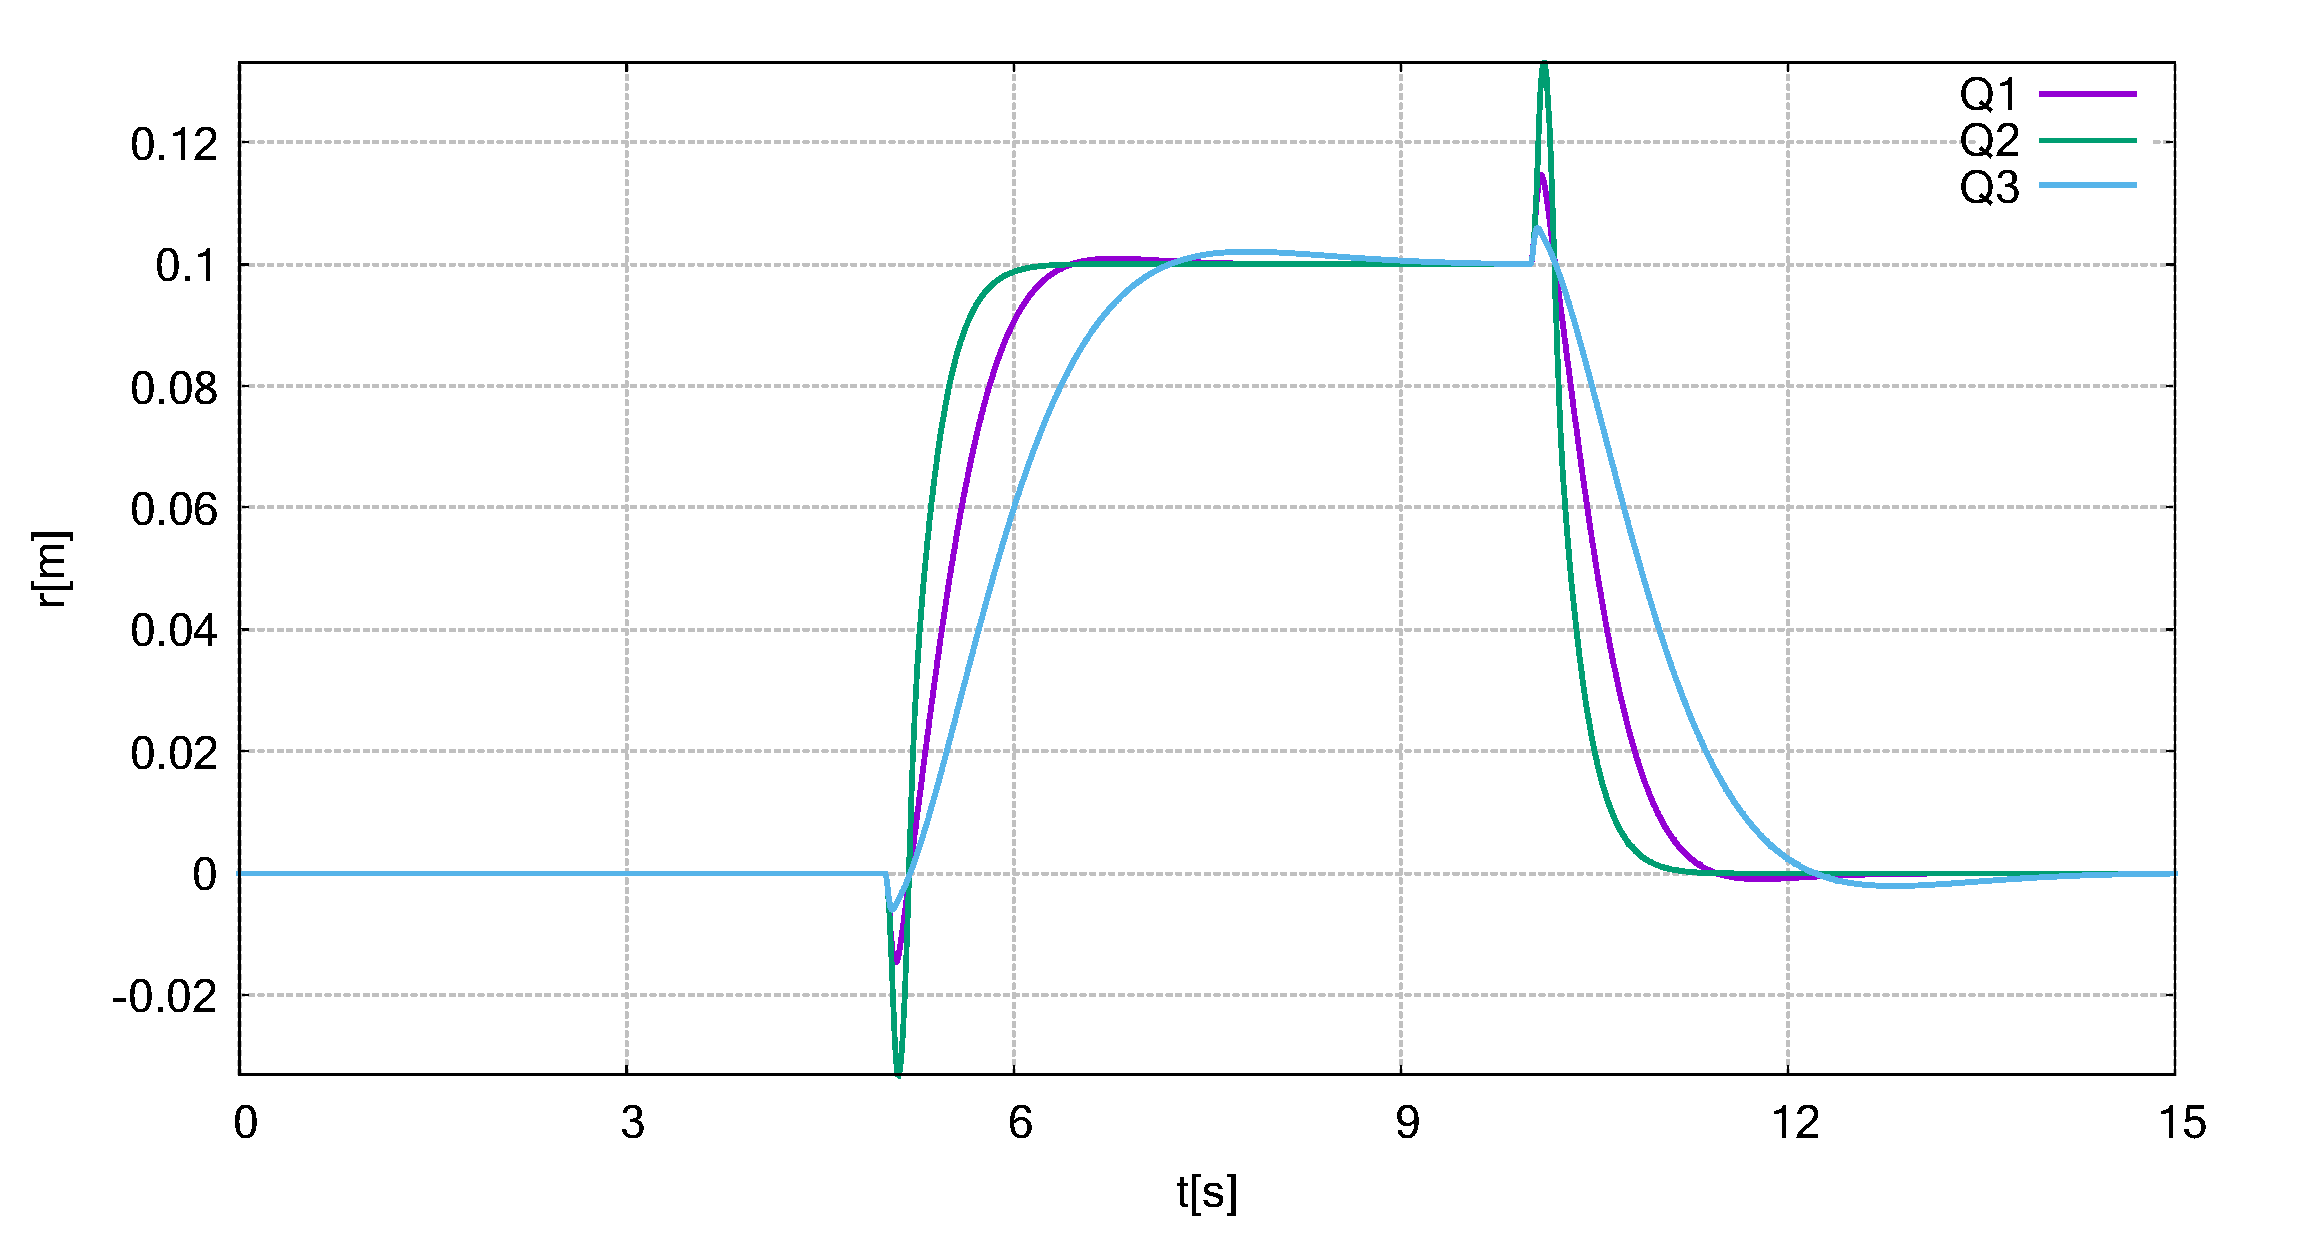
\includegraphics[width=0.8\linewidth]{gazo/simulation_QRF_compare_R.eps}
		\caption{重み行列での比較結果(台車位置)}
		\label{image:simulation_QRF_r}
	\end{figure}
	\begin{figure}[H]
		\centering
		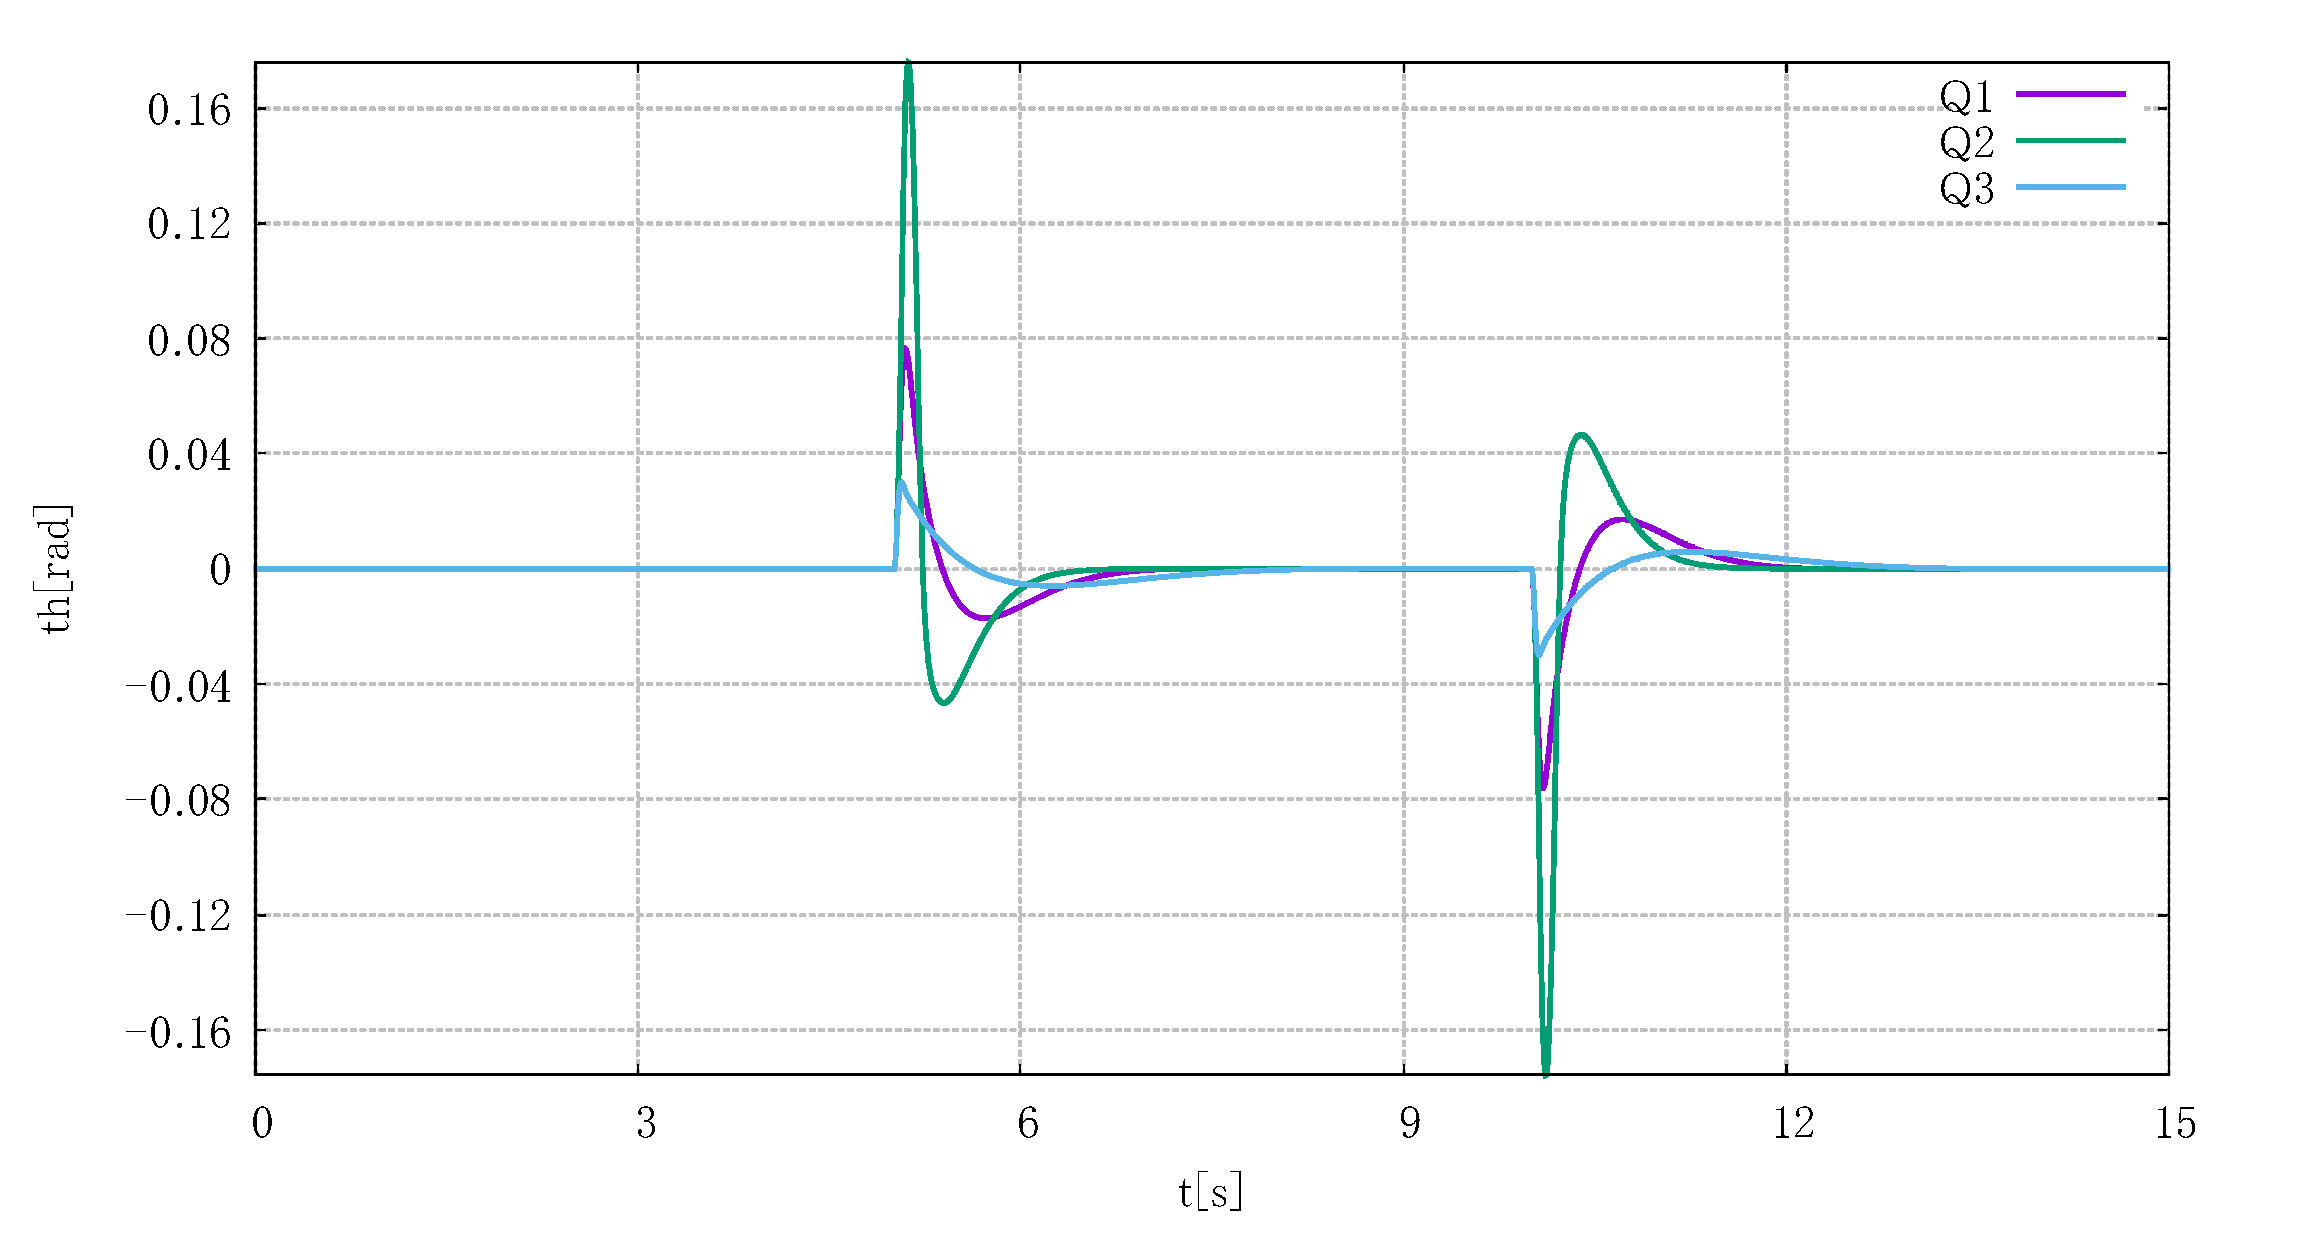
\includegraphics[width=0.8\linewidth]{gazo/simulation_QRF_compare_THETA.eps}
		\caption{重み行列での比較結果(振子角度)}
		\label{image:simulation_QRF_th}
	\end{figure}
	%図のほう要確認
	図(\ref{image:simulation_QRF_r})より$Q_2$の応答が一番早く、$Q_3$の応答が一番遅いことが確認できる。このことから台車の位置$r$の応答をよくするには
	重み行列$Q$の第1成分を大きくすればよいとわかる。また、$Q_1$と$Q_3$の第1成分は同じであるのにもかかわらず、$Q_1$の方が応答が早いことが確認できる。これは
	振子の角度$\theta$の応答をよくする第2成分を大きくした分、バランスが第2成分のほうに偏ってしまい、台車の位置の応答が悪くなったといえる。
	\par
	図(\ref{image:simulation_QRF_th})より、振子の角度についても同じことが言え、第2成分を大きくしている$Q_3$の応答が一番よく、$Q_2$の応答が一番悪い結果となっている。
	\par
	以上から重み行列の調整については以下のことが言える。
	\begin{itemize}
	  \item 重み行列$Q$の各成分は$r,\theta,\dot{r},\dot{\theta}$に対応している
	  \item 応答をよくしたい状態があれば、その状態に対応する成分の値を大きくすればよい
	  \item その場合、大きくした成分に対応する状態にバランスが偏る(つまり、ほかの状態の応答が悪くなる)
	\end{itemize}
	
	
% --------------------------------------------------------------------------------------
\section{オブザーバの極の変更による制御性能評価}
	前章で述べたように、最小次元オブザーバを設計するためにゴピナスの方法を用いる。
	この時、システム行列$A$、入力行列$B$、出力行列$C$、オブザーバの極$P$が必要である。
	オブザーバの極$P$を調整することで倒立振子の安定化制御の性能を高めることができる。
	同様にシミュレーションによって制御性能を考察していく。
	\par
	1つ考慮しなければならないのは、オブザーバの極と
	閉ループ系の極(つまり、$(A-BF)$の固有値)との位置関係である。
	閉ループ系の極のうち虚軸に最も近い極を$\lambda_{max}$としたとき、オブザーバーの極$P$は
	\[
		\rm{Re}(P) <5\rm{Re}(\lambda_{max})
	\]
	を満たす考慮して設定する必要がある。
	表(\ref{table:QRF})の$Q_2$を用いて設計した状態フィードバック$F$における閉ループ系の極は
	\begin{equation}
		D=\left[
		\begin{array}{c}
			-0.08\\
			-6.3+1.3i\\
			-6.3+1.3i\\
			-13\\
		\end{array}
		\right]
		\label{eq:Aeig}
	\end{equation}
	である。この中で一番虚軸に近い極は$-0.08$である。よって、少なくともオブザーバーの極$P$は$-0.4$
	より小さい値をとればよいとわかる。
	\par
	以下にシミュレーションを行う異なるパターンのパラメータをまとめた表とその時のシミュレーション結果を示す。
	\begin{table}[htb]
		\begin{center}
			\caption{オブザーバの極の変更パターン}
			\medskip
			
			\begin{tabular}{|c|c|c|c|}\hline
				\ \ & 重み行列$Q$ & オブザーバの極$P$ & サンプリング周期$\Delta[\rm{s}]$ \\ \hline\hline
				パターン1 & $Q_1$:$\rm{diag}(1E5,1E5,1,1)$ & $P_1$:$((-60,0),(-60,0))^{'}$ & $\Delta_1$:0.005 \\ \hline
				パターン2 & $Q_1$:$\rm{diag}(1E5,1E5,1,1)$ & $P_2$:$((-30,0),(-30,0))^{'}$ & $\Delta_1$:0.005 \\ \hline
			\end{tabular}
		\end{center}
		\label{table:QRF}
	\end{table}
	
	\begin{figure}[H]
		\centering
		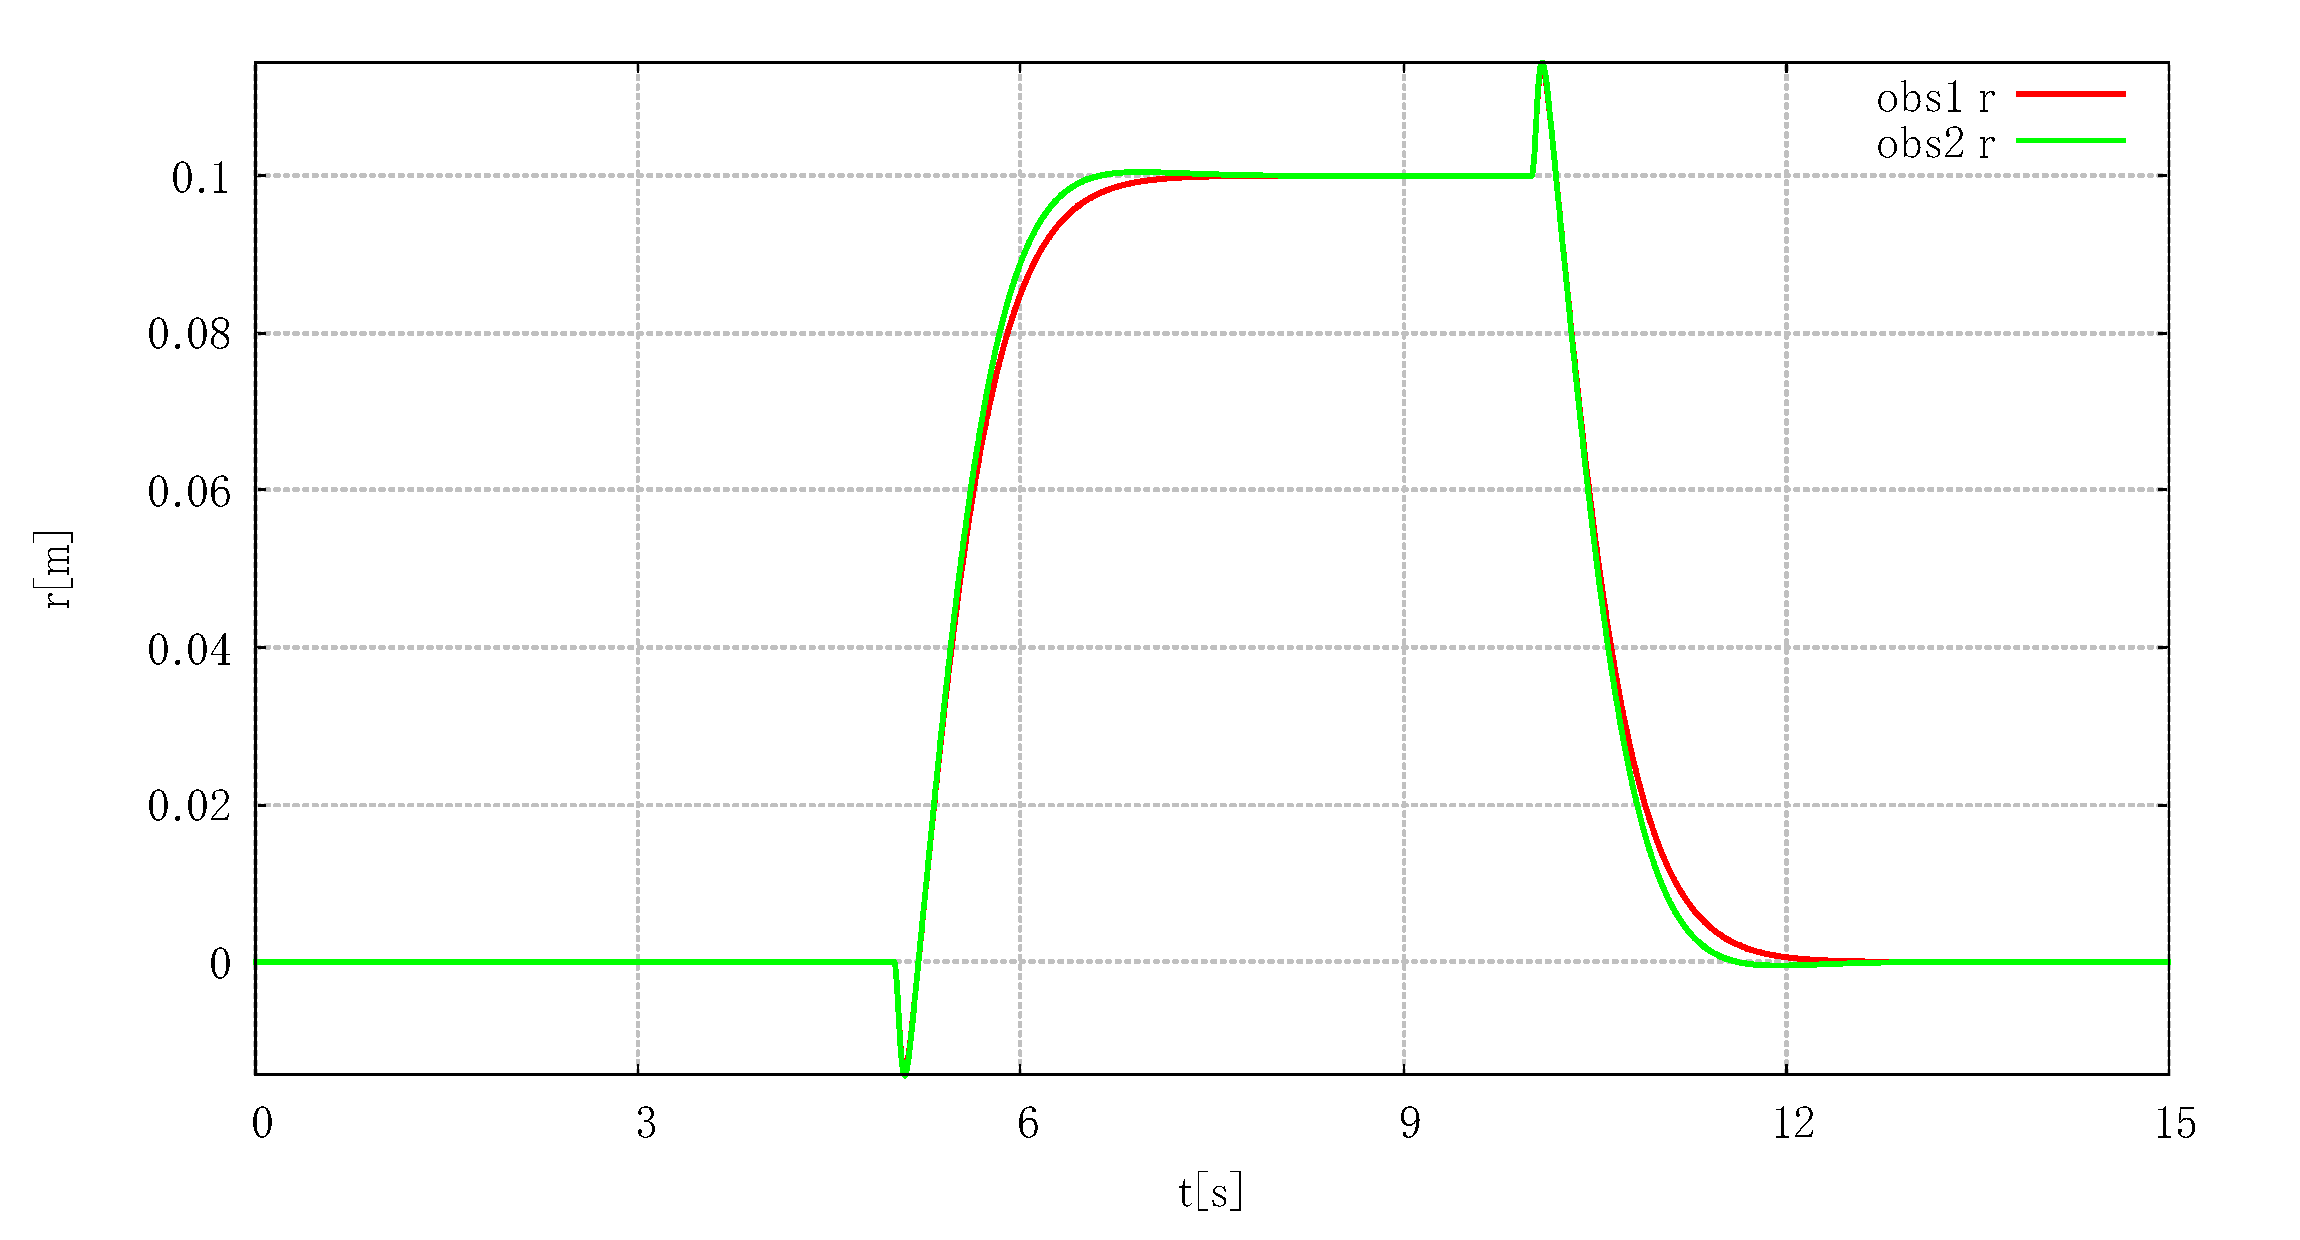
\includegraphics[width=0.8\linewidth]{gazo/simulation_obs_compare_R.eps}
		\caption{オブザーバーの極での比較結果(台車位置)}
		\label{image:simulation_obs_r}
	\end{figure}
	\begin{figure}[H]
		\centering
		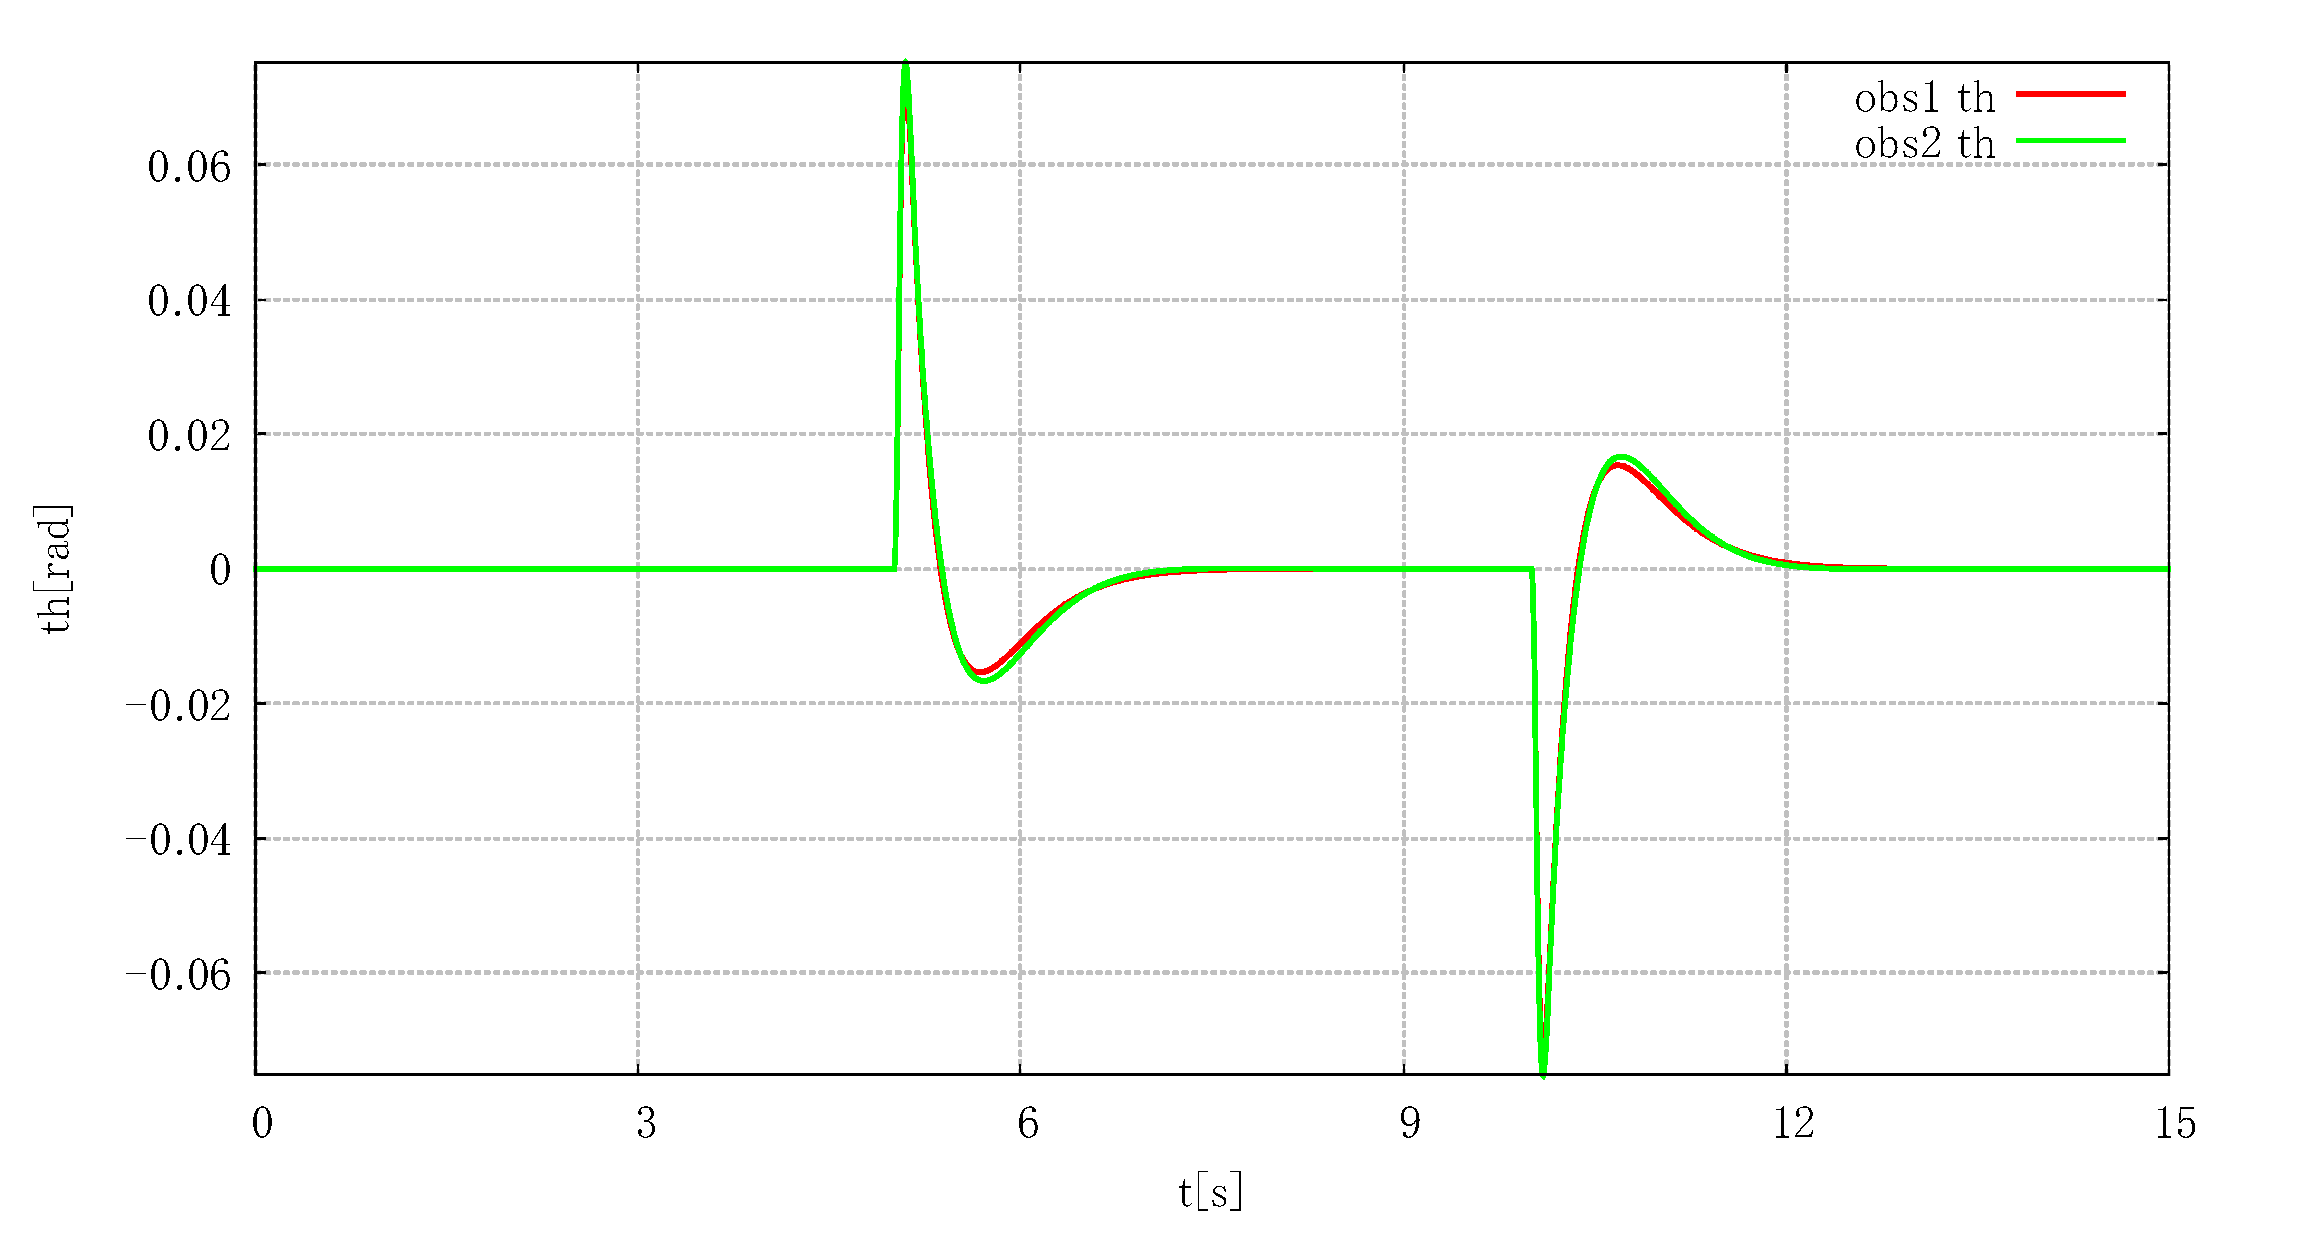
\includegraphics[width=0.8\linewidth]{gazo/simulation_obs_compare_THETA.eps}
		\caption{オブザーバーの極での比較結果(振子角度)}
		\label{image:simulation_obs_theta}
	\end{figure} 
	図\ref{image:simulation_obs_r}と図\ref{image:simulation_obs_theta}よりオブザーバの極の違いによる大きな違いは確認できない。
	ここで、倒立振子の状態$x(t)$(台車の速度と振り子の角速度)とオブザーバで推定した値$\hat{x}[k・T]$(台車の速度と振り子の角速度)
	との差である推定誤差($x(t)-\hat{x}[K・T]$)の応答波形からオブザーバの極の違いによる考察をする。
	以下に台車の速度と振り子の角速度の推定誤差の図を示す。
	\begin{figure}[H]
		\centering
		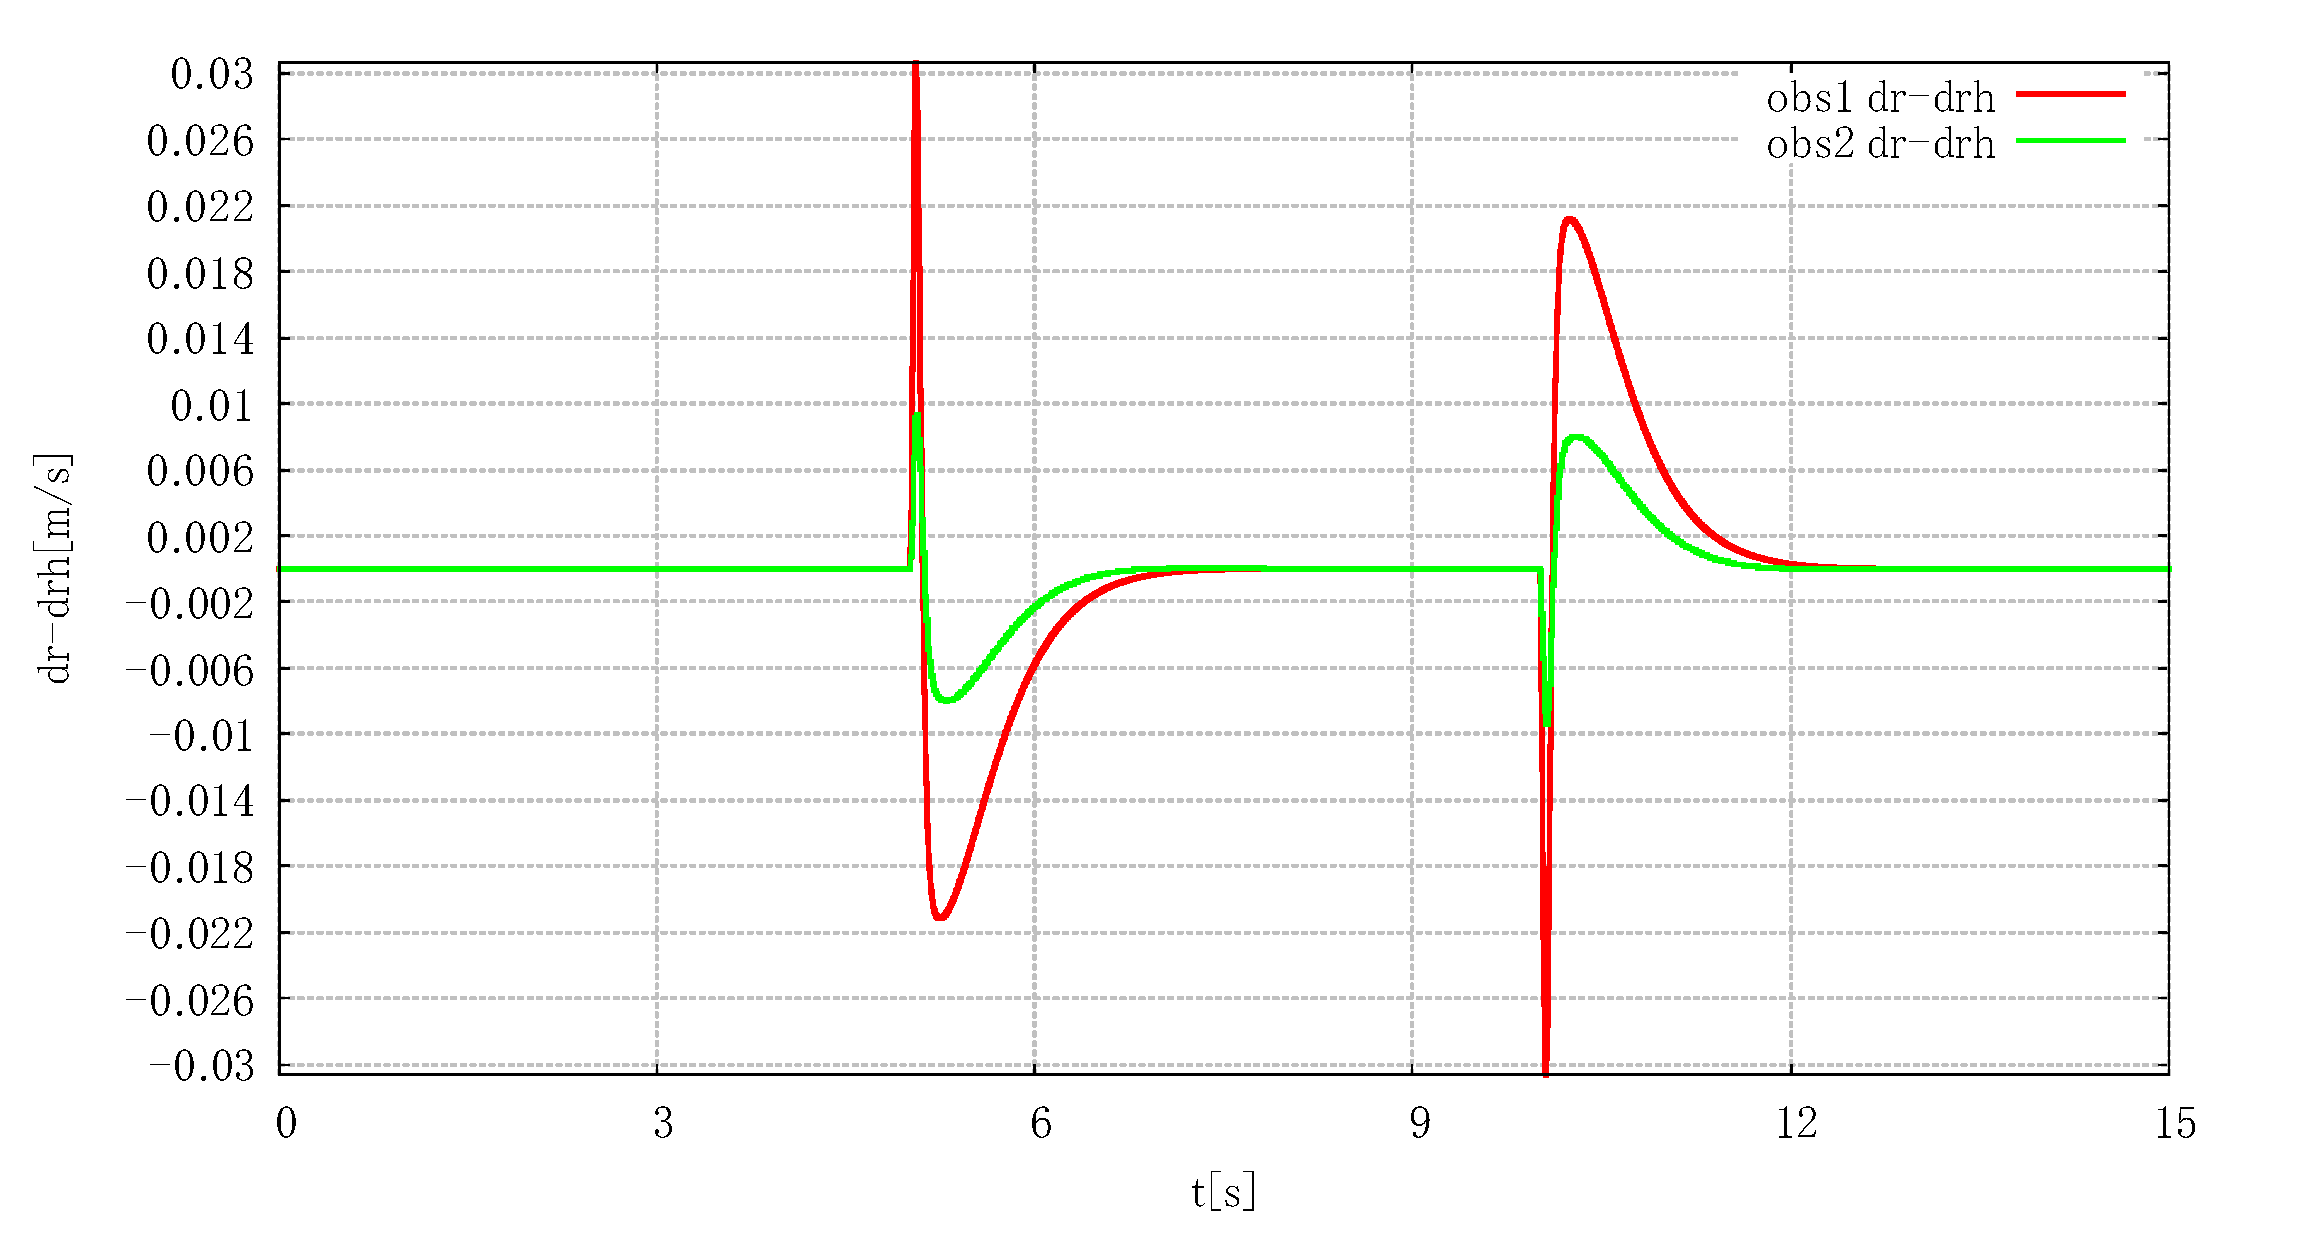
\includegraphics[width=0.8\linewidth]{gazo/simulation_obs_compare_RminusRH.eps}
		\caption{オブザーバーの極での推定誤差の比較(台車の速度)}
		\label{image:simulation_obs_rminusrh}
	\end{figure}
	\begin{figure}[H]
		\centering
		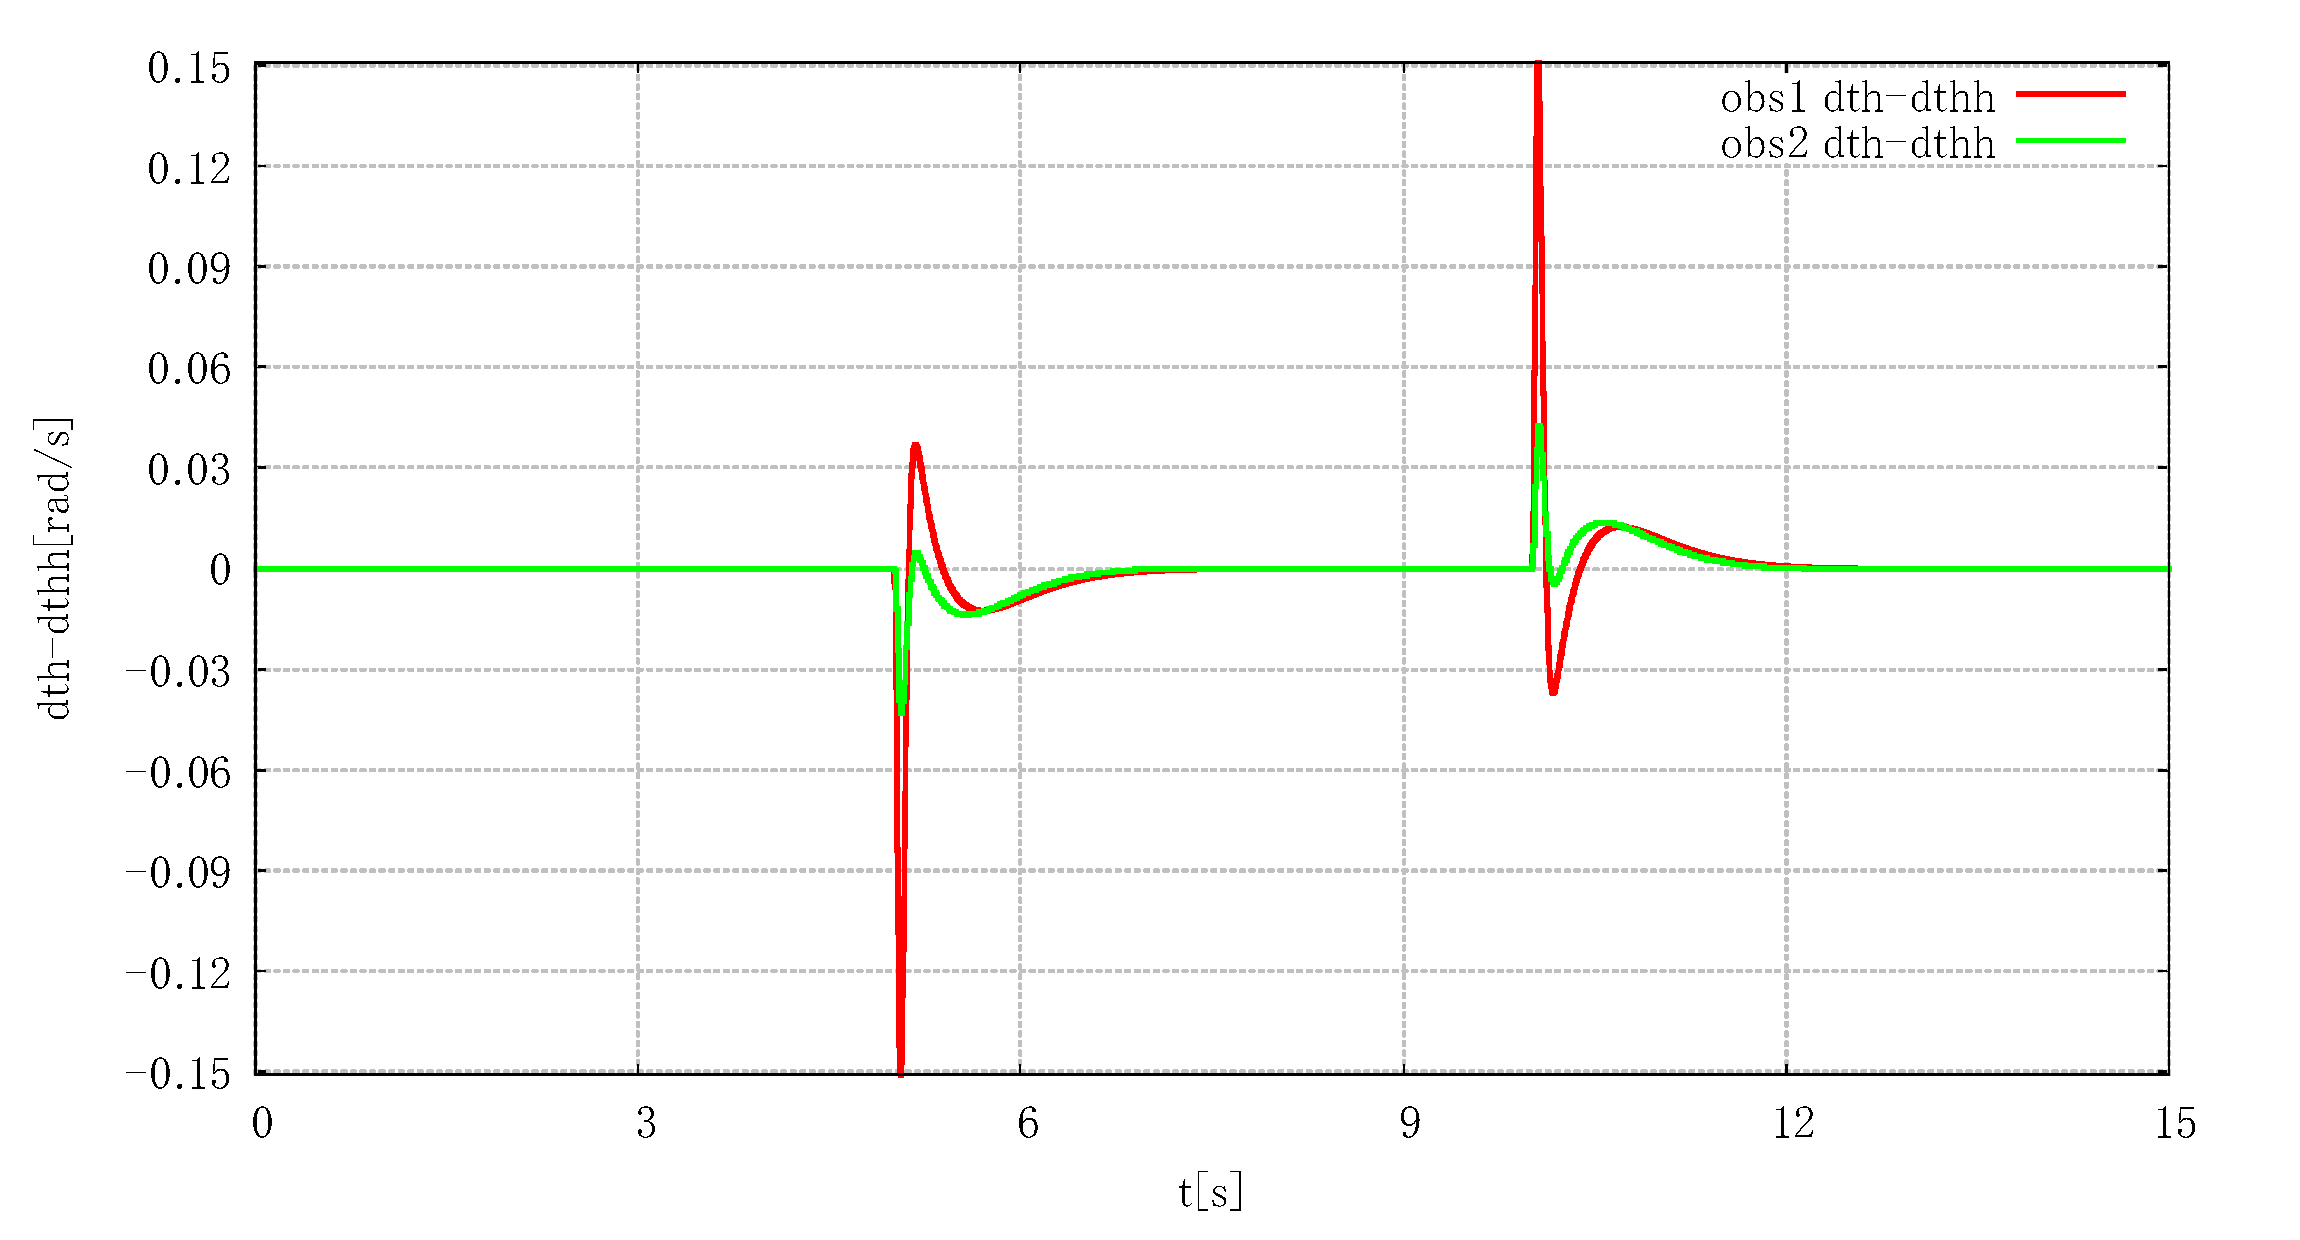
\includegraphics[width=0.8\linewidth]{gazo/simulation_obs_compare_THETAminusTHETAH.eps}
		\caption{オブザーバーの極での推定誤差の比較(振子の角速度)}
		\label{image:simulation_obs_thetaminusthetah}
	\end{figure} 
	図\ref{image:simulation_obs_rminusrh}と図\ref{image:simulation_obs_thetaminusthetah}よりオブザーバの極が
	虚軸から遠いパターン2のほうが推定誤差の収束が若干遅いことがわかる。また、その大きさもパターン2のほうが大きいこともわかる。
	\par
	以上からオブザーバの極配置の調整については以下のことが言える。
	\begin{itemize}
	  \item オブザーバの極は虚軸に近いほうが推定誤差が小さくなり応答はよくなるといえる。
	  \item ただし、閉ループ系の極との位置関係を考慮するひつようがある。
	\end{itemize}
	
%--------------------------------------------------------------------------------------
\section{サンプリング周期の変更による制御性能評価}
	離散化を行うサンプリング周期$\Delta$を調整することで倒立振子の安定化制御の性能を高めることができる。
	同様にシミュレーションによって制御性能を考察していく。
	ただし、サンプリング周期が短すぎると実験で用いる倒立振子系においてシステム全体がハングアップする恐れ
	があるため、そのような値においてはシミュレーションを行わない。
	\par
	以下にシミュレーションを行う異なるパターンのパラメータをまとめた表とその時のシミュレーション結果を示す。
	\begin{table}[htb]
		\begin{center}
			\caption{サンプリング周期の変更パターン}
			\medskip
			
			\begin{tabular}{|c|c|c|c|}\hline
				& 重み行列$Q$ & オブザーバの極$P$ & サンプリング周期$\Delta[\rm{s}]$ \\ \hline\hline
				パターン1 & $Q_1$:$\rm{diag}(1E5,1E5,1,1)$ & $P_1$:$((-60,0),(-60,0))^{'}$ & $\Delta_1$:0.005 \\ \hline
				パターン2 & $Q_1$:$\rm{diag}(1E5,1E5,1,1)$ & $P_1$:$((-60,0),(-60,0))^{'}$ & $\Delta_2$:0.01 \\ \hline
			\end{tabular}
		\end{center}
		\label{table:QRF}
	\end{table}
	
	\begin{figure}[H]
		\centering
		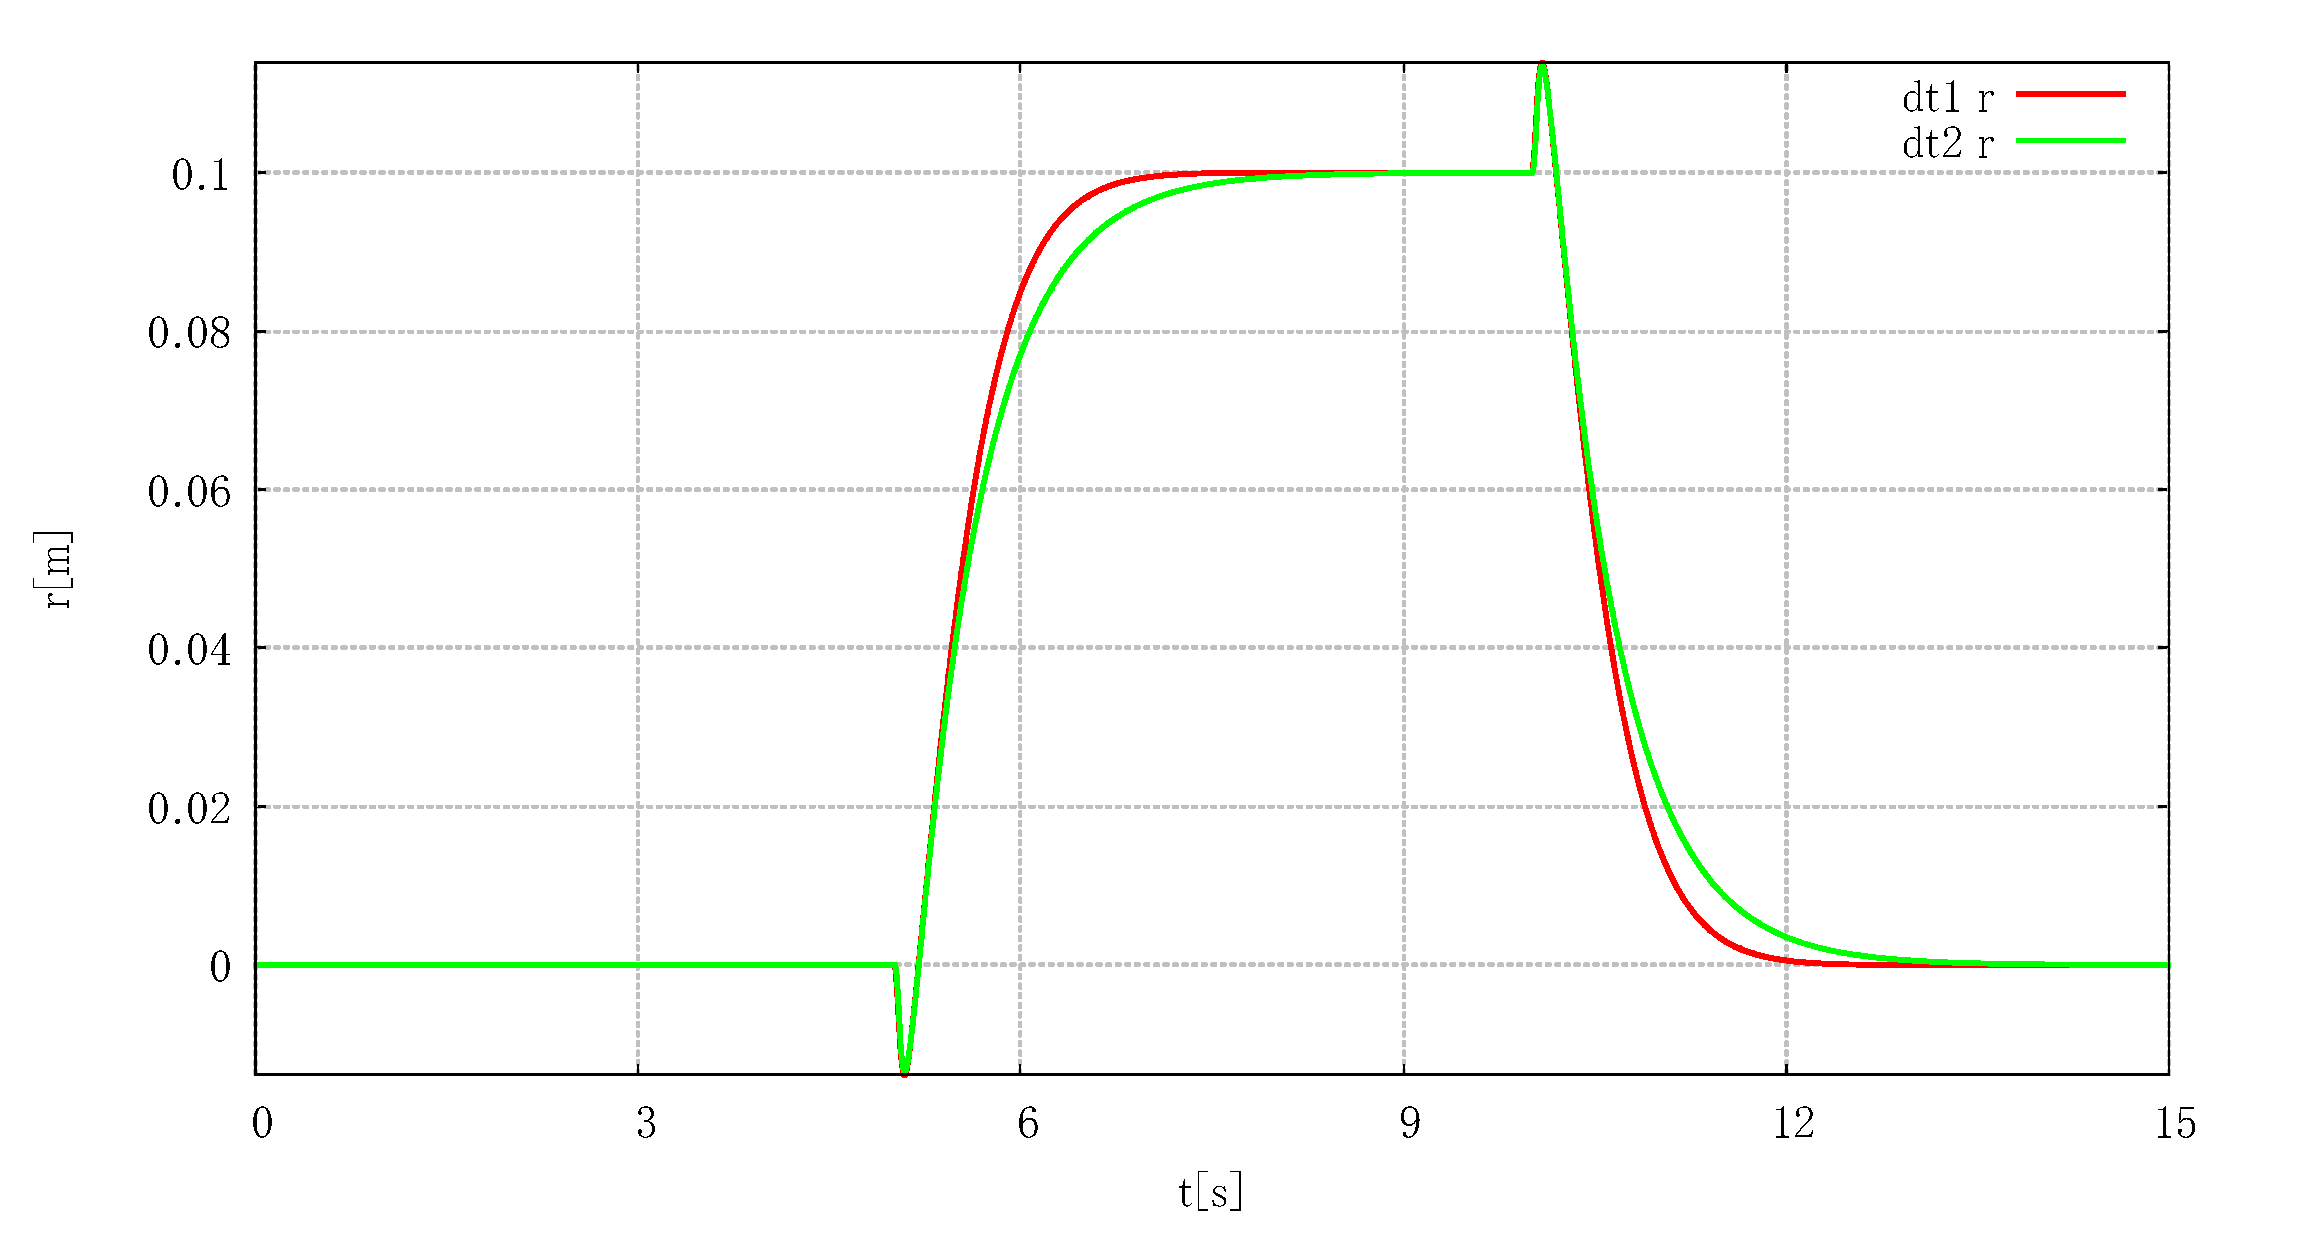
\includegraphics[width=0.8\linewidth]{gazo/simulation_dt_compare_R.eps}
		\caption{サンプリング周期での比較結果(台車位置)}
		\label{image:simulation_dt_r}
	\end{figure}
	\begin{figure}[H]
		\centering
		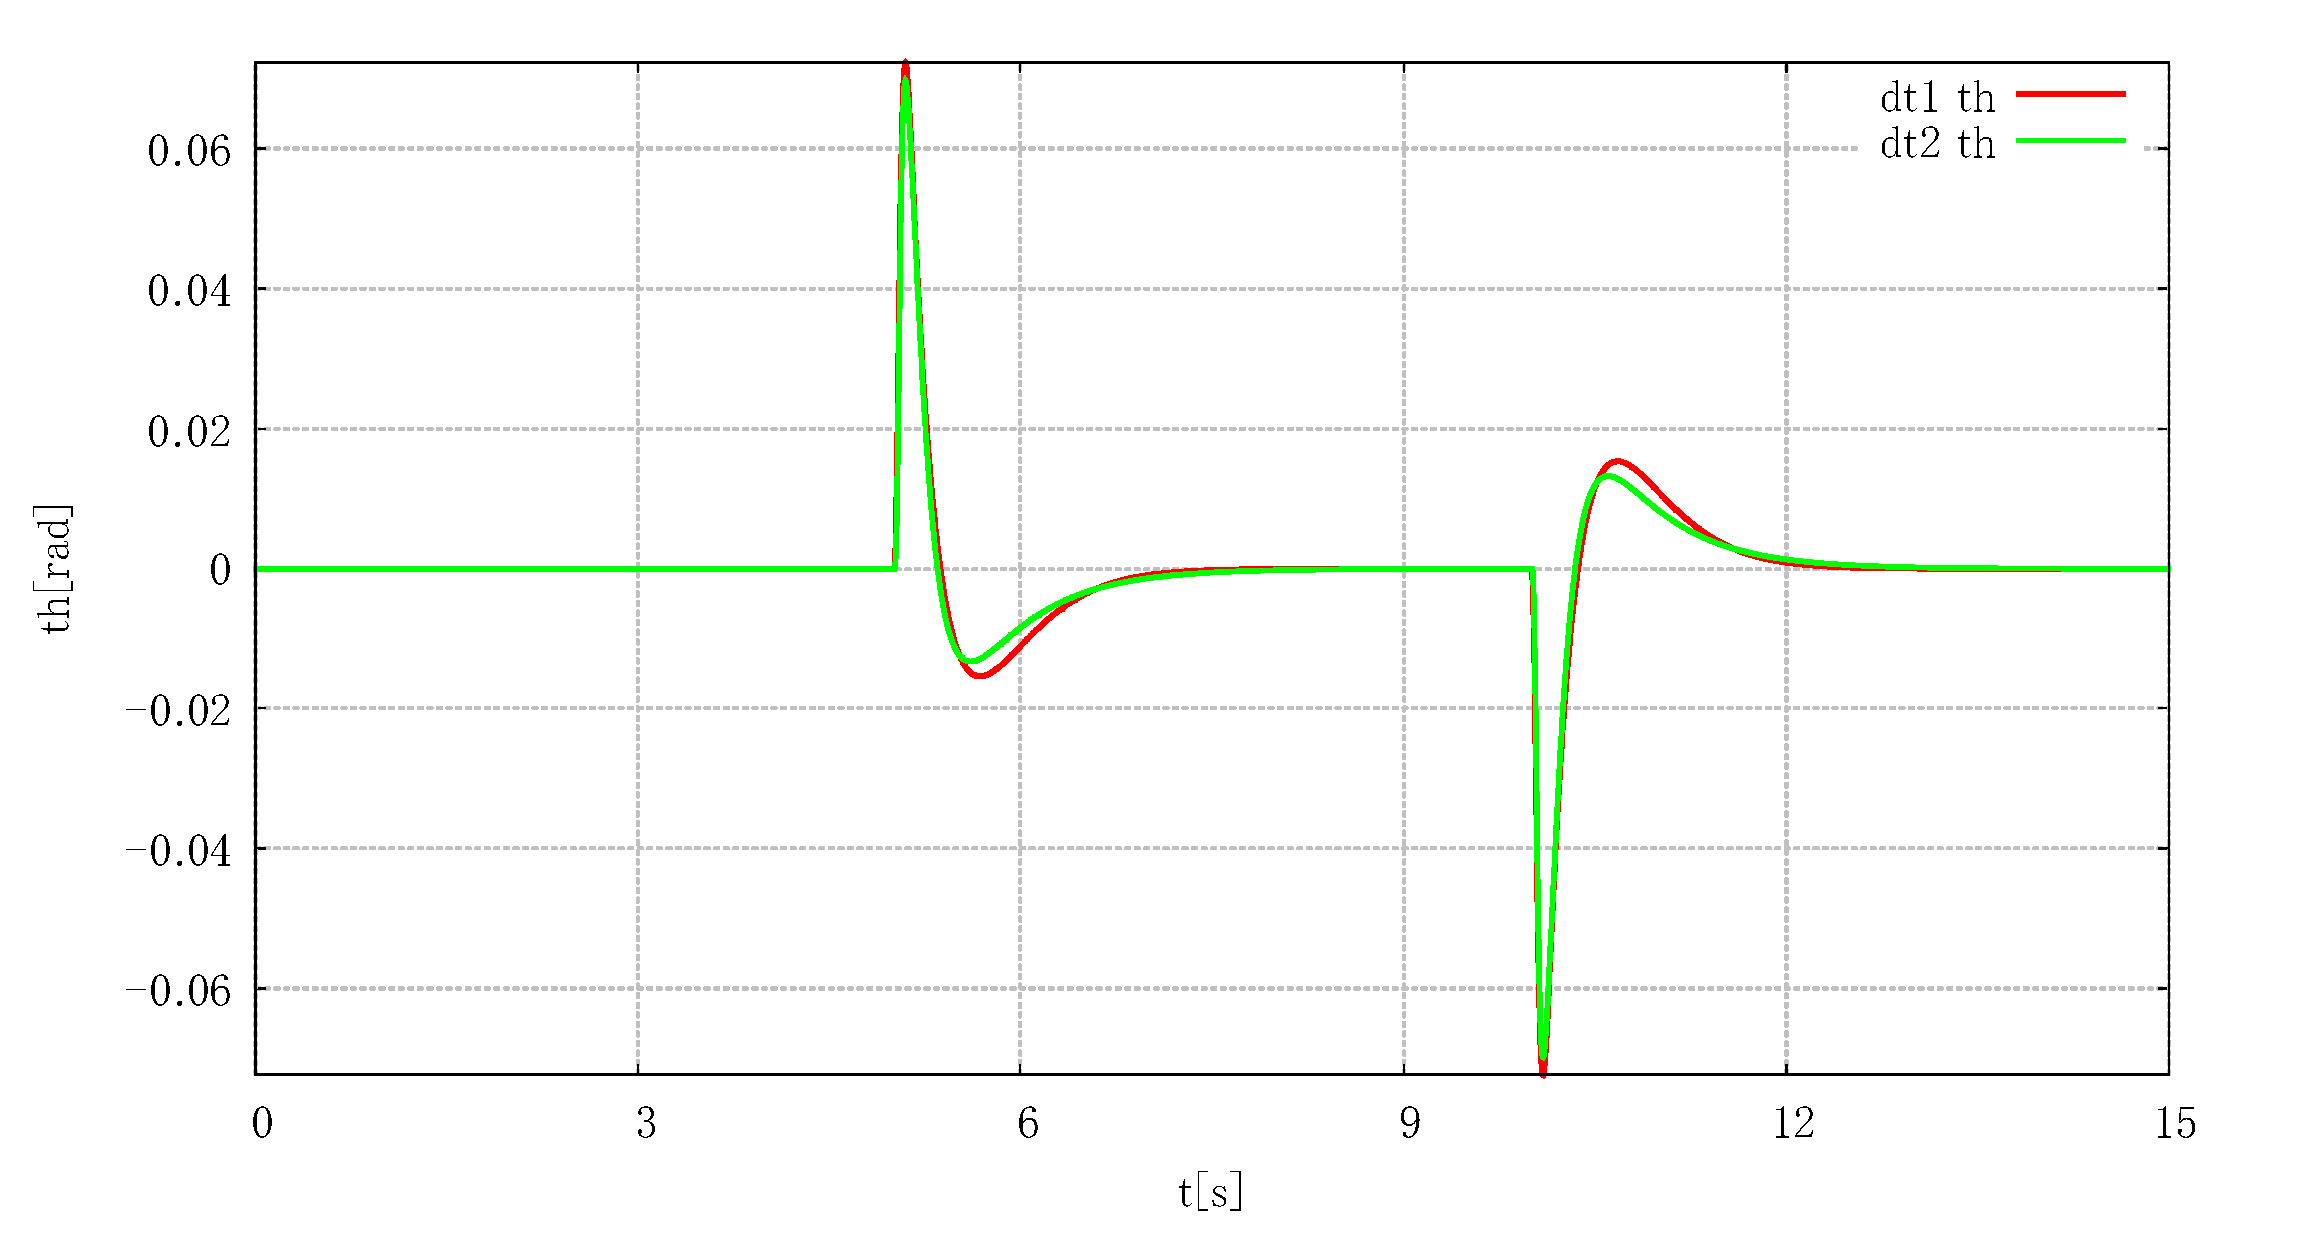
\includegraphics[width=0.8\linewidth]{gazo/simulation_dt_compare_THETA.eps}
		\caption{サンプリング周期での比較結果(振子角度)}
		\label{image:simulation_dt_theta}
	\end{figure}
	図\ref{image:simulation_dt_r}から、パターン1のほうが若干応答が早いといえる。しかし、
	図\ref{image:simulation_dt_r}と図\ref{image:simulation_dt_theta}からは大きな違いを確認することはできない。
	先ほどと同様に推定誤差の応答波形からサンプリング周期の違いによる考察をする。
	以下に台車の速度と振り子の角速度の推定誤差の図を示す。
	\begin{figure}[H]
		\centering
		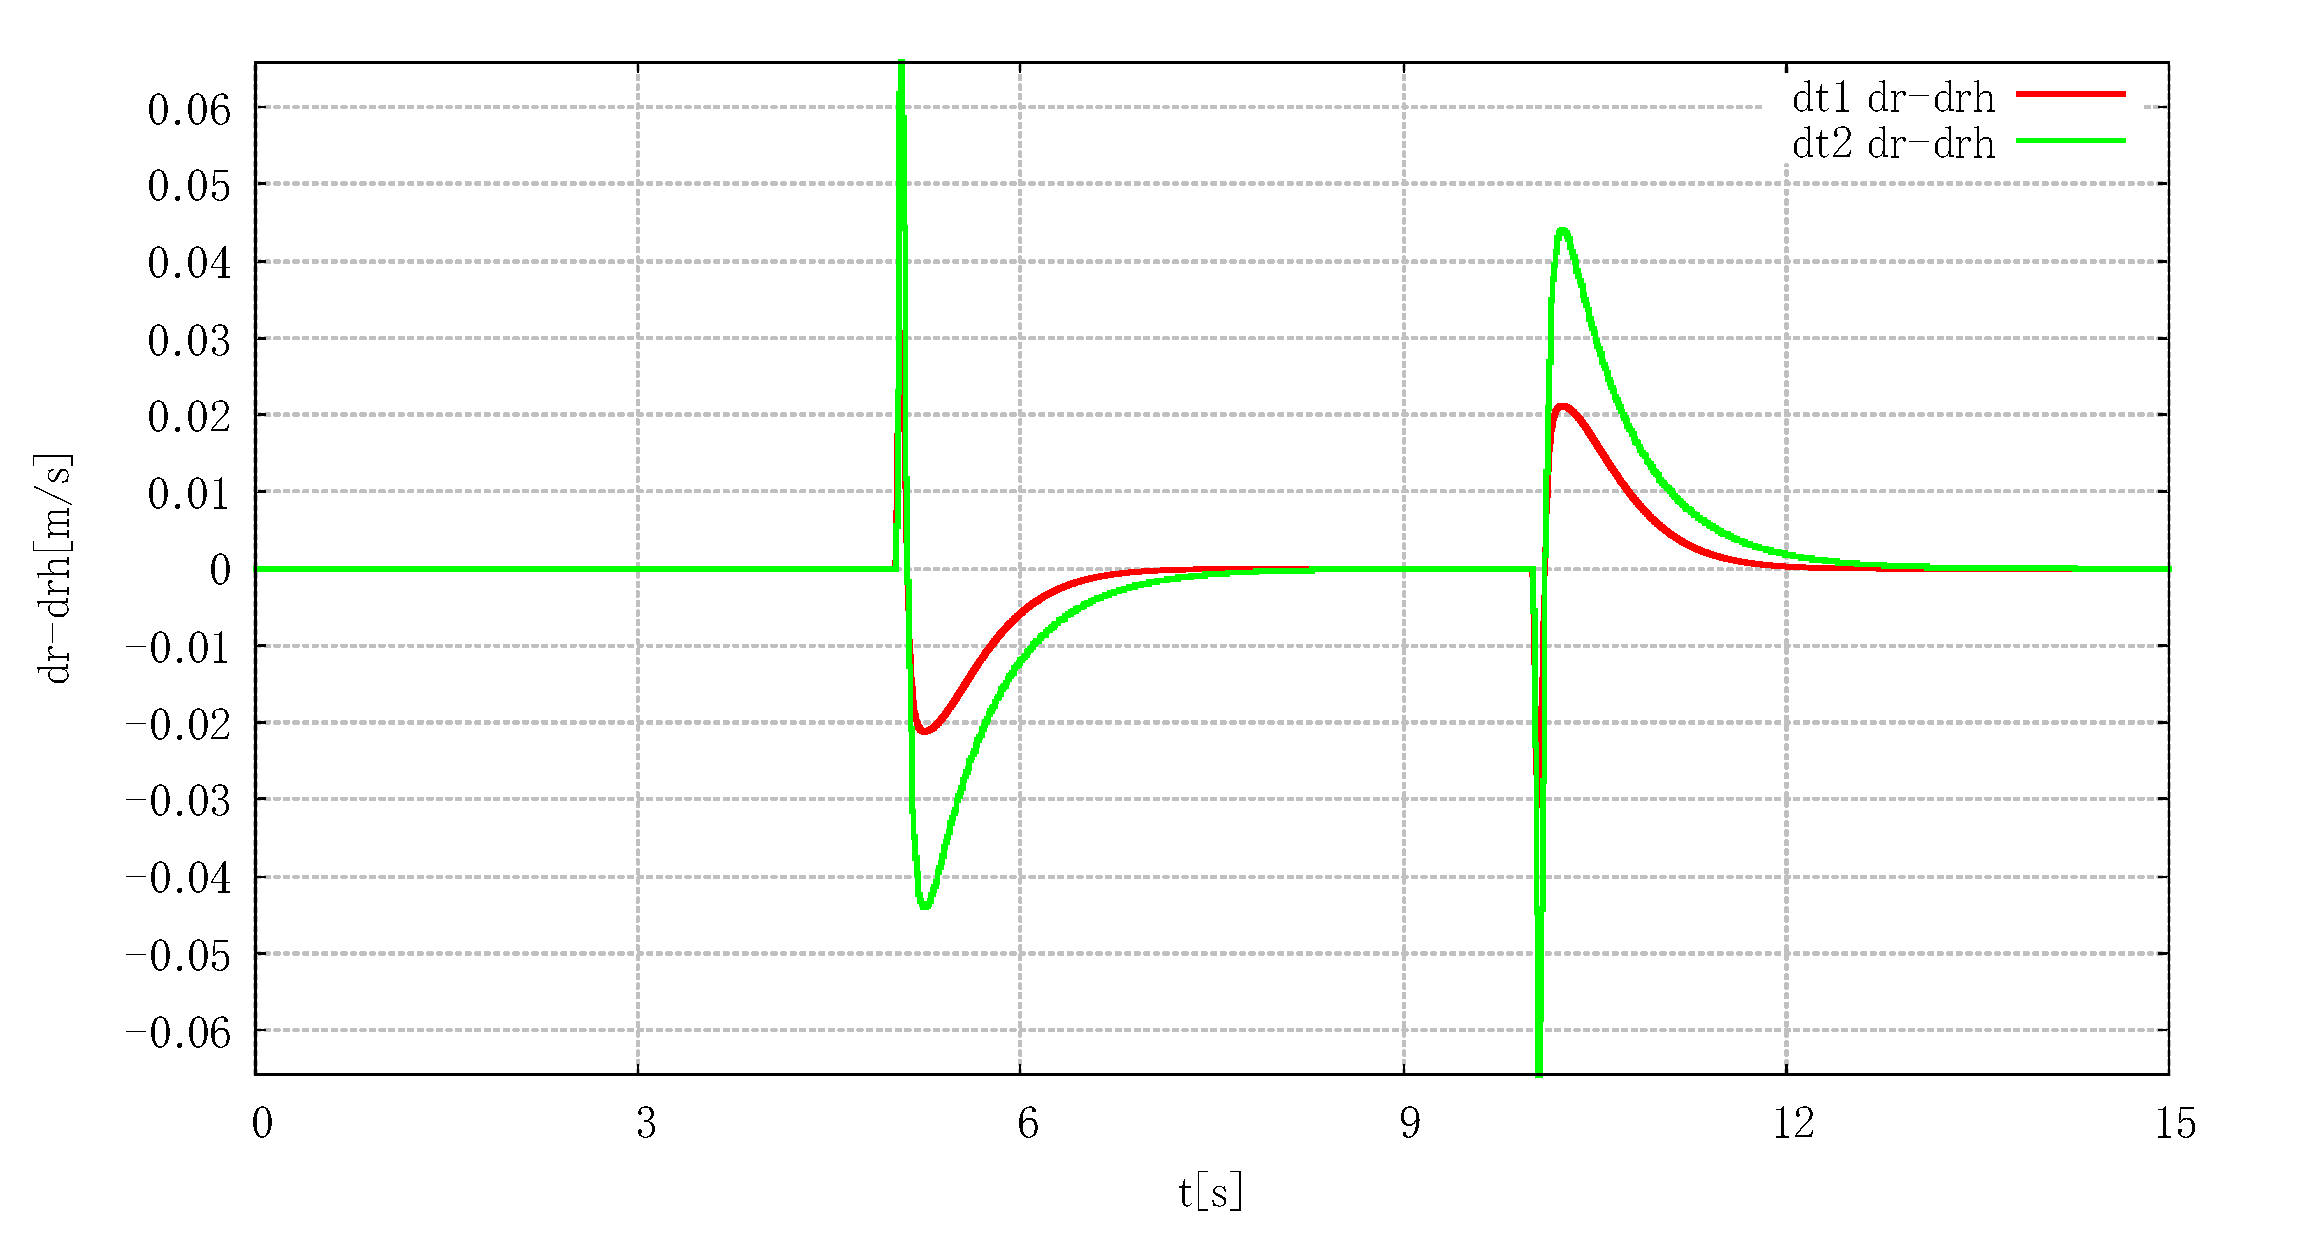
\includegraphics[width=0.8\linewidth]{gazo/simulation_dt_compare_RminusRH.eps}
		\caption{サンプリング周期での推定誤差の比較(台車の速度)}
		\label{image:simulation_dt_rminusrh}
	\end{figure}
	\begin{figure}[H]
		\centering
		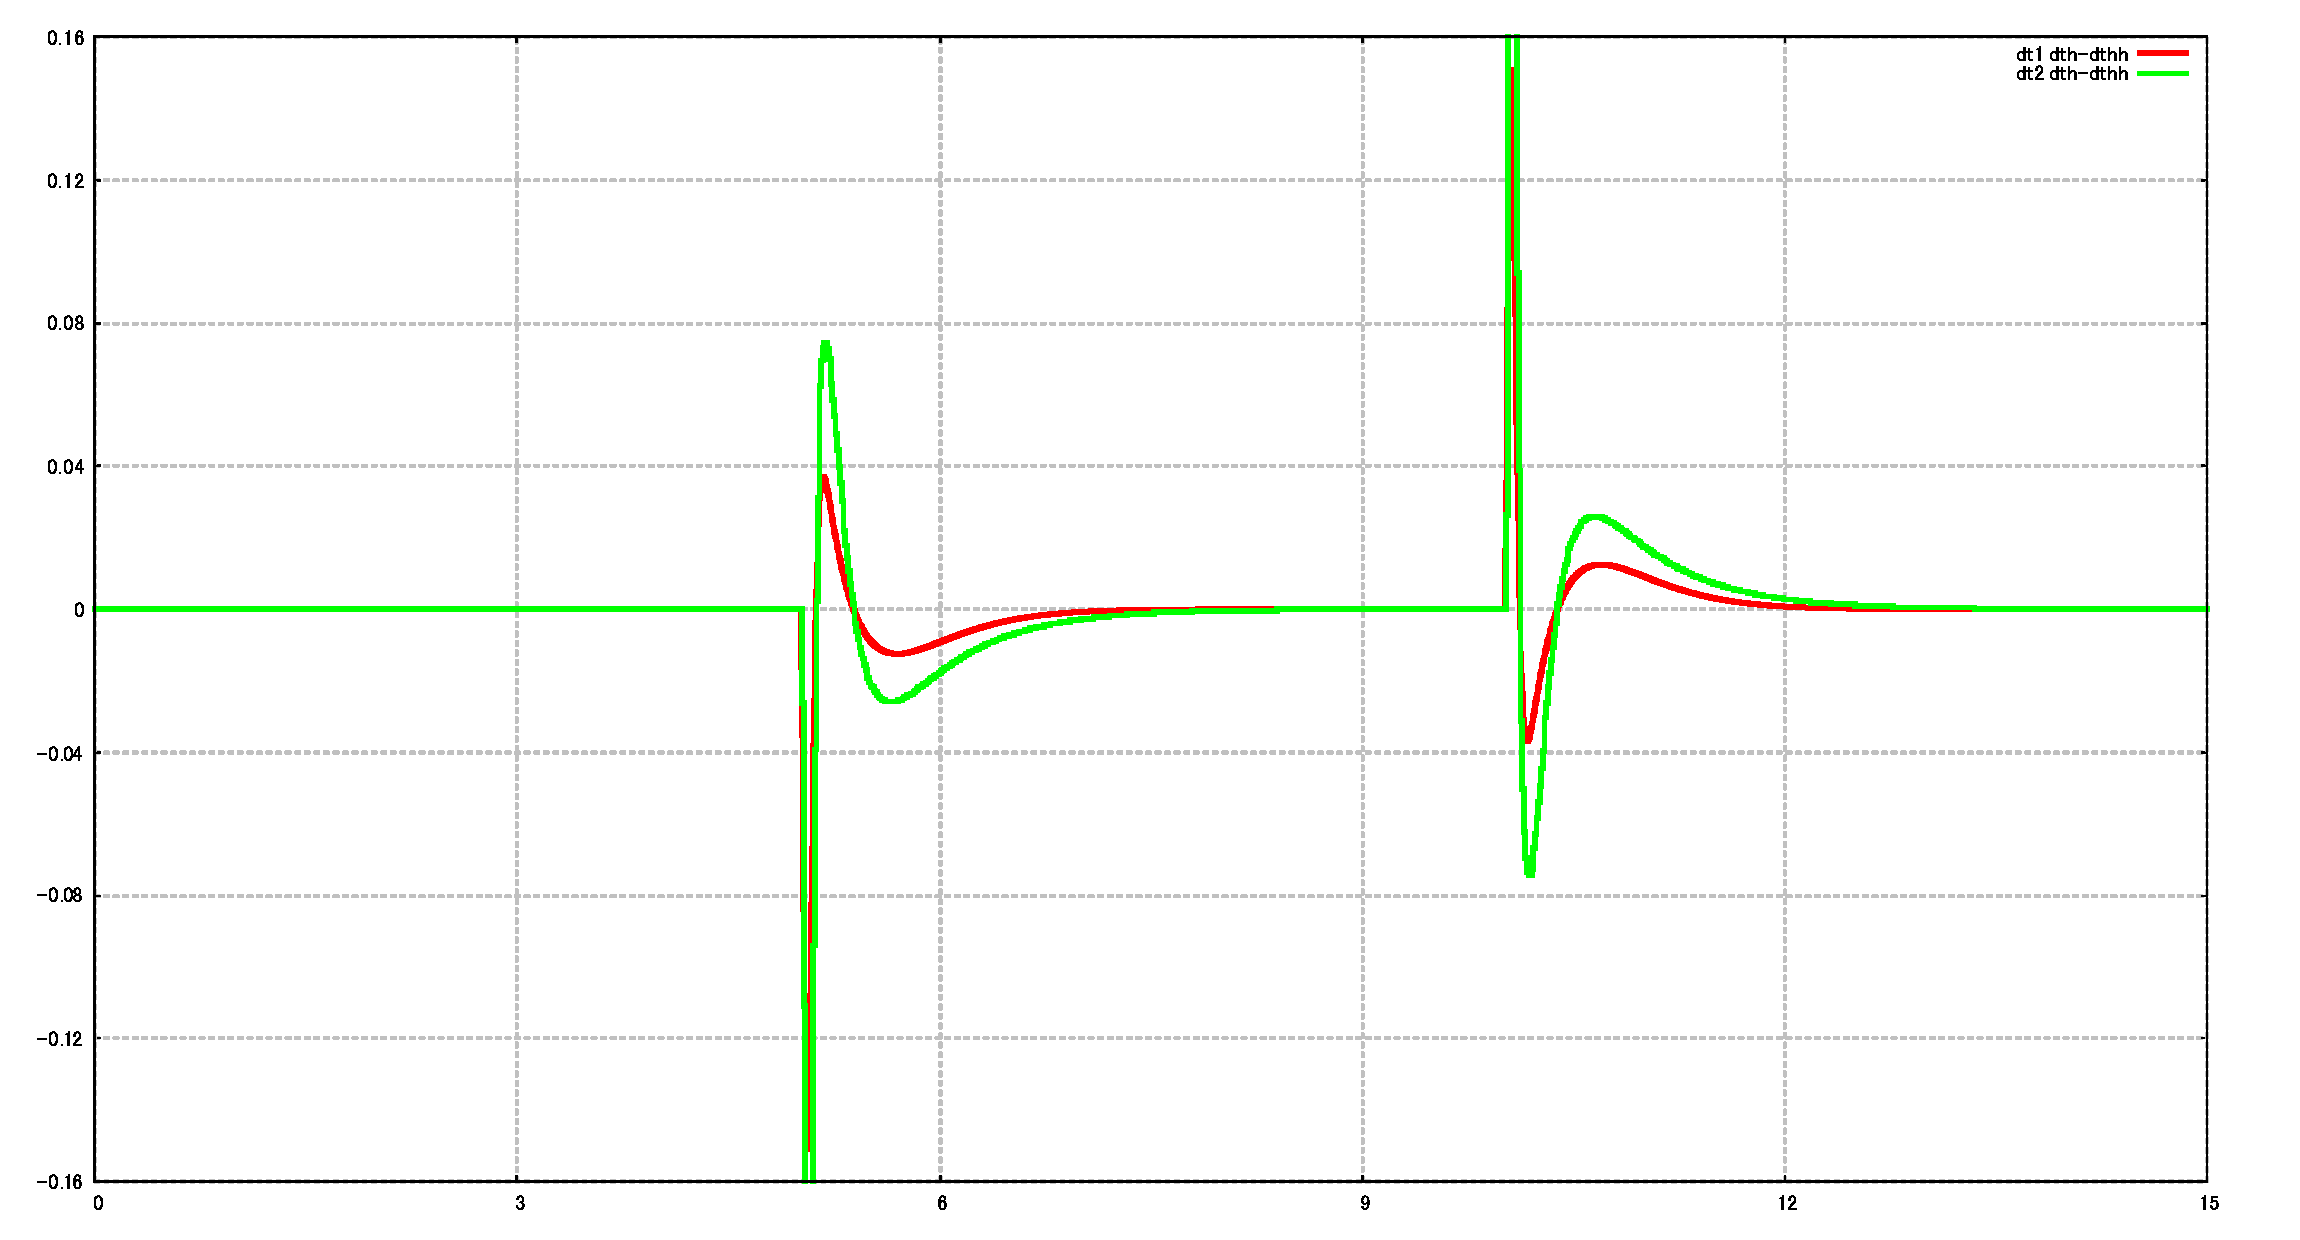
\includegraphics[width=0.8\linewidth]{gazo/simulation_dt_compare_THETAminusTHETAH.eps}
		\caption{サンプリング周期での推定誤差の比較(振子の各速度)}
		\label{image:simulation_dt_thetaminusthetah}
	\end{figure}
	図\ref{image:simulation_dt_rminusrh}と図\ref{image:simulation_dt_thetaminusthetah}よりサンプリング周期の短いほうが
	推定誤差が小さいことが確認できる。
	\par
	以上からサンプリング周期の調整については以下のことが言える。
	\begin{itemize}
	  \item サンプリング周期は短いほうが推定誤差が小さくなり、応答がよくなる。
	  \item ただし、あまり小さくしすぎるのはよくない。
	\end{itemize}
	
%--------------------------------------------------------------------------------------
\section{振り上げ制御及び安定化に対する制御性能評価}
	前節までにおいて、安定化制御における有効なパラメータを考察してきた。
	ここでは、振り上げ制御におけるパラメータ$k,n$を調整することで振り上げ制御の制御性能を考察する。
	\par
	この時、安定化制御に用いるパラメータは以下の表の通りである。
	安定化制御の際に使用するパラメータについてはこれまでの考察に基づいて決定した。
	\begin{table}[htb]
		\begin{center}
			\caption{振り上げ後の安定化制御の際に用いるパラメータの組}
			\medskip
			
			\begin{tabular}{|c|c|c|c|}\hline
				重み行列$Q$ & オブザーバの極$P$ & サンプリング周期$\Delta[\rm{s}]$ \\ \hline\hline
				$Q_1$:$\rm{diag}(1E5,1E5,1,1)$ & $P_1$:$((-30,0),(-30,0))^{'}$ & $\Delta_1$:0.005 \\ \hline
			\end{tabular}
		\end{center}
		\label{table:huriage_control}
	\end{table}
	振り上げ制御に用いるパラメータは以下の表の通りである。
	\begin{table}[H]
		\begin{center}
			\caption{振り上げ制御に用いるパラメータの組}
			\medskip
			
			\begin{tabular}{|c|c|c|}\hline
				& $n$ & $k$ \\ \hline\hline
				パターン1 & 0.4 & $1.0×10^3$  \\ \hline
				パターン2 & 0.4 & $1.0×10^4$  \\ \hline
				パターン3 & 0.4 & $1.0×10^5$  \\ \hline
			\end{tabular}
		\end{center}
		\label{table:huriage_huriage}
	\end{table}
	以上の表のパラメータを用いて行ったシミュレーションの結果を示す。
	\begin{figure}[H]
		\centering
		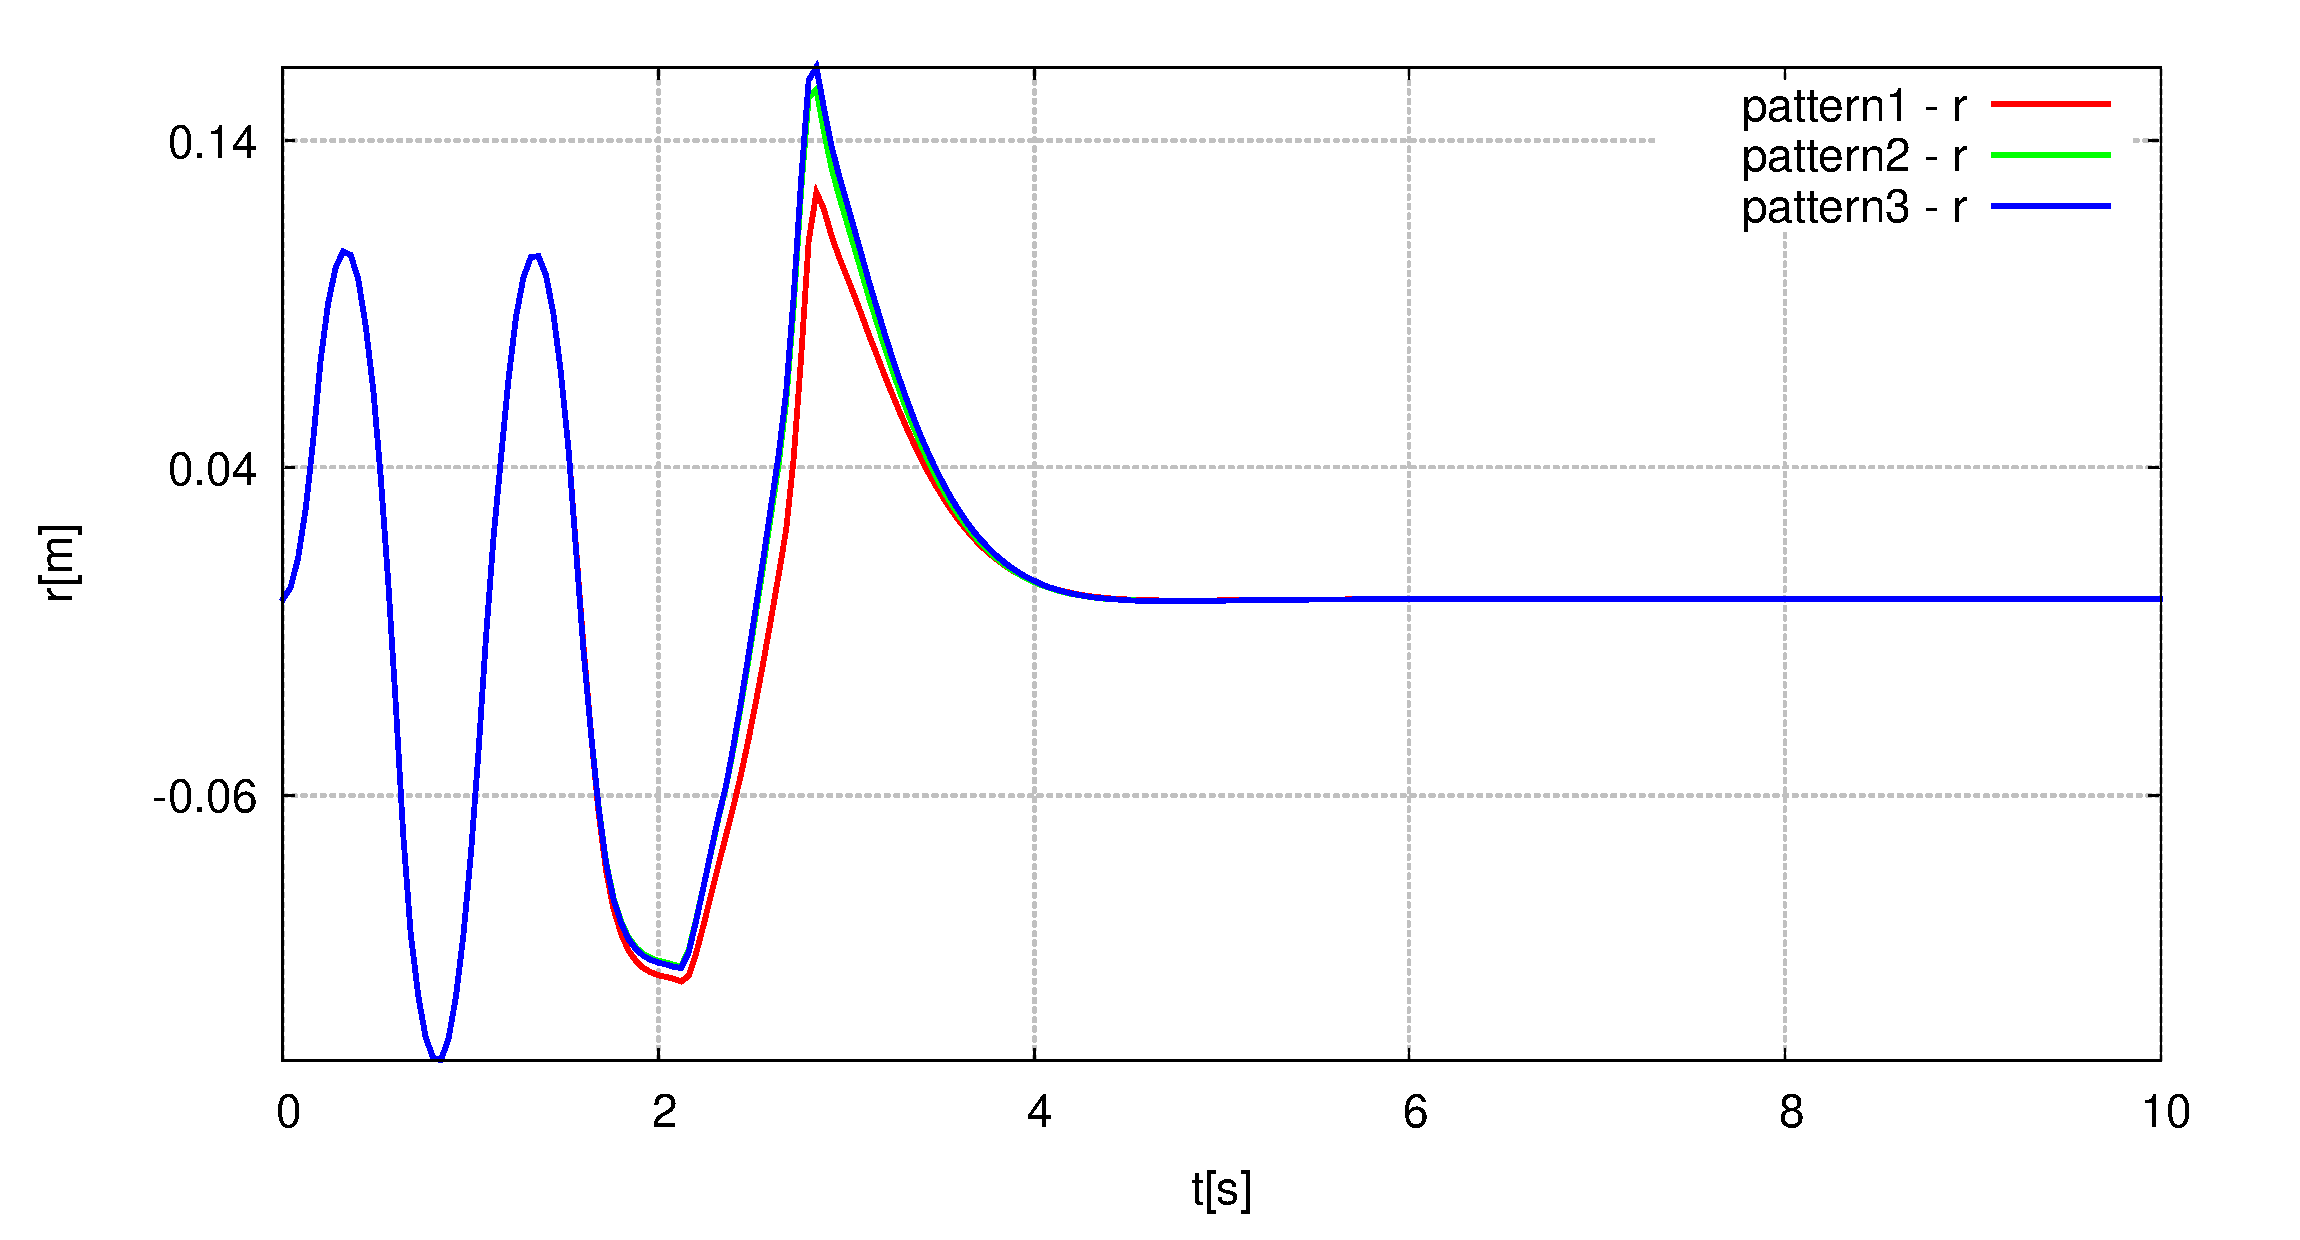
\includegraphics[width=0.4\linewidth]{gazo/Hsimu_R.eps}
		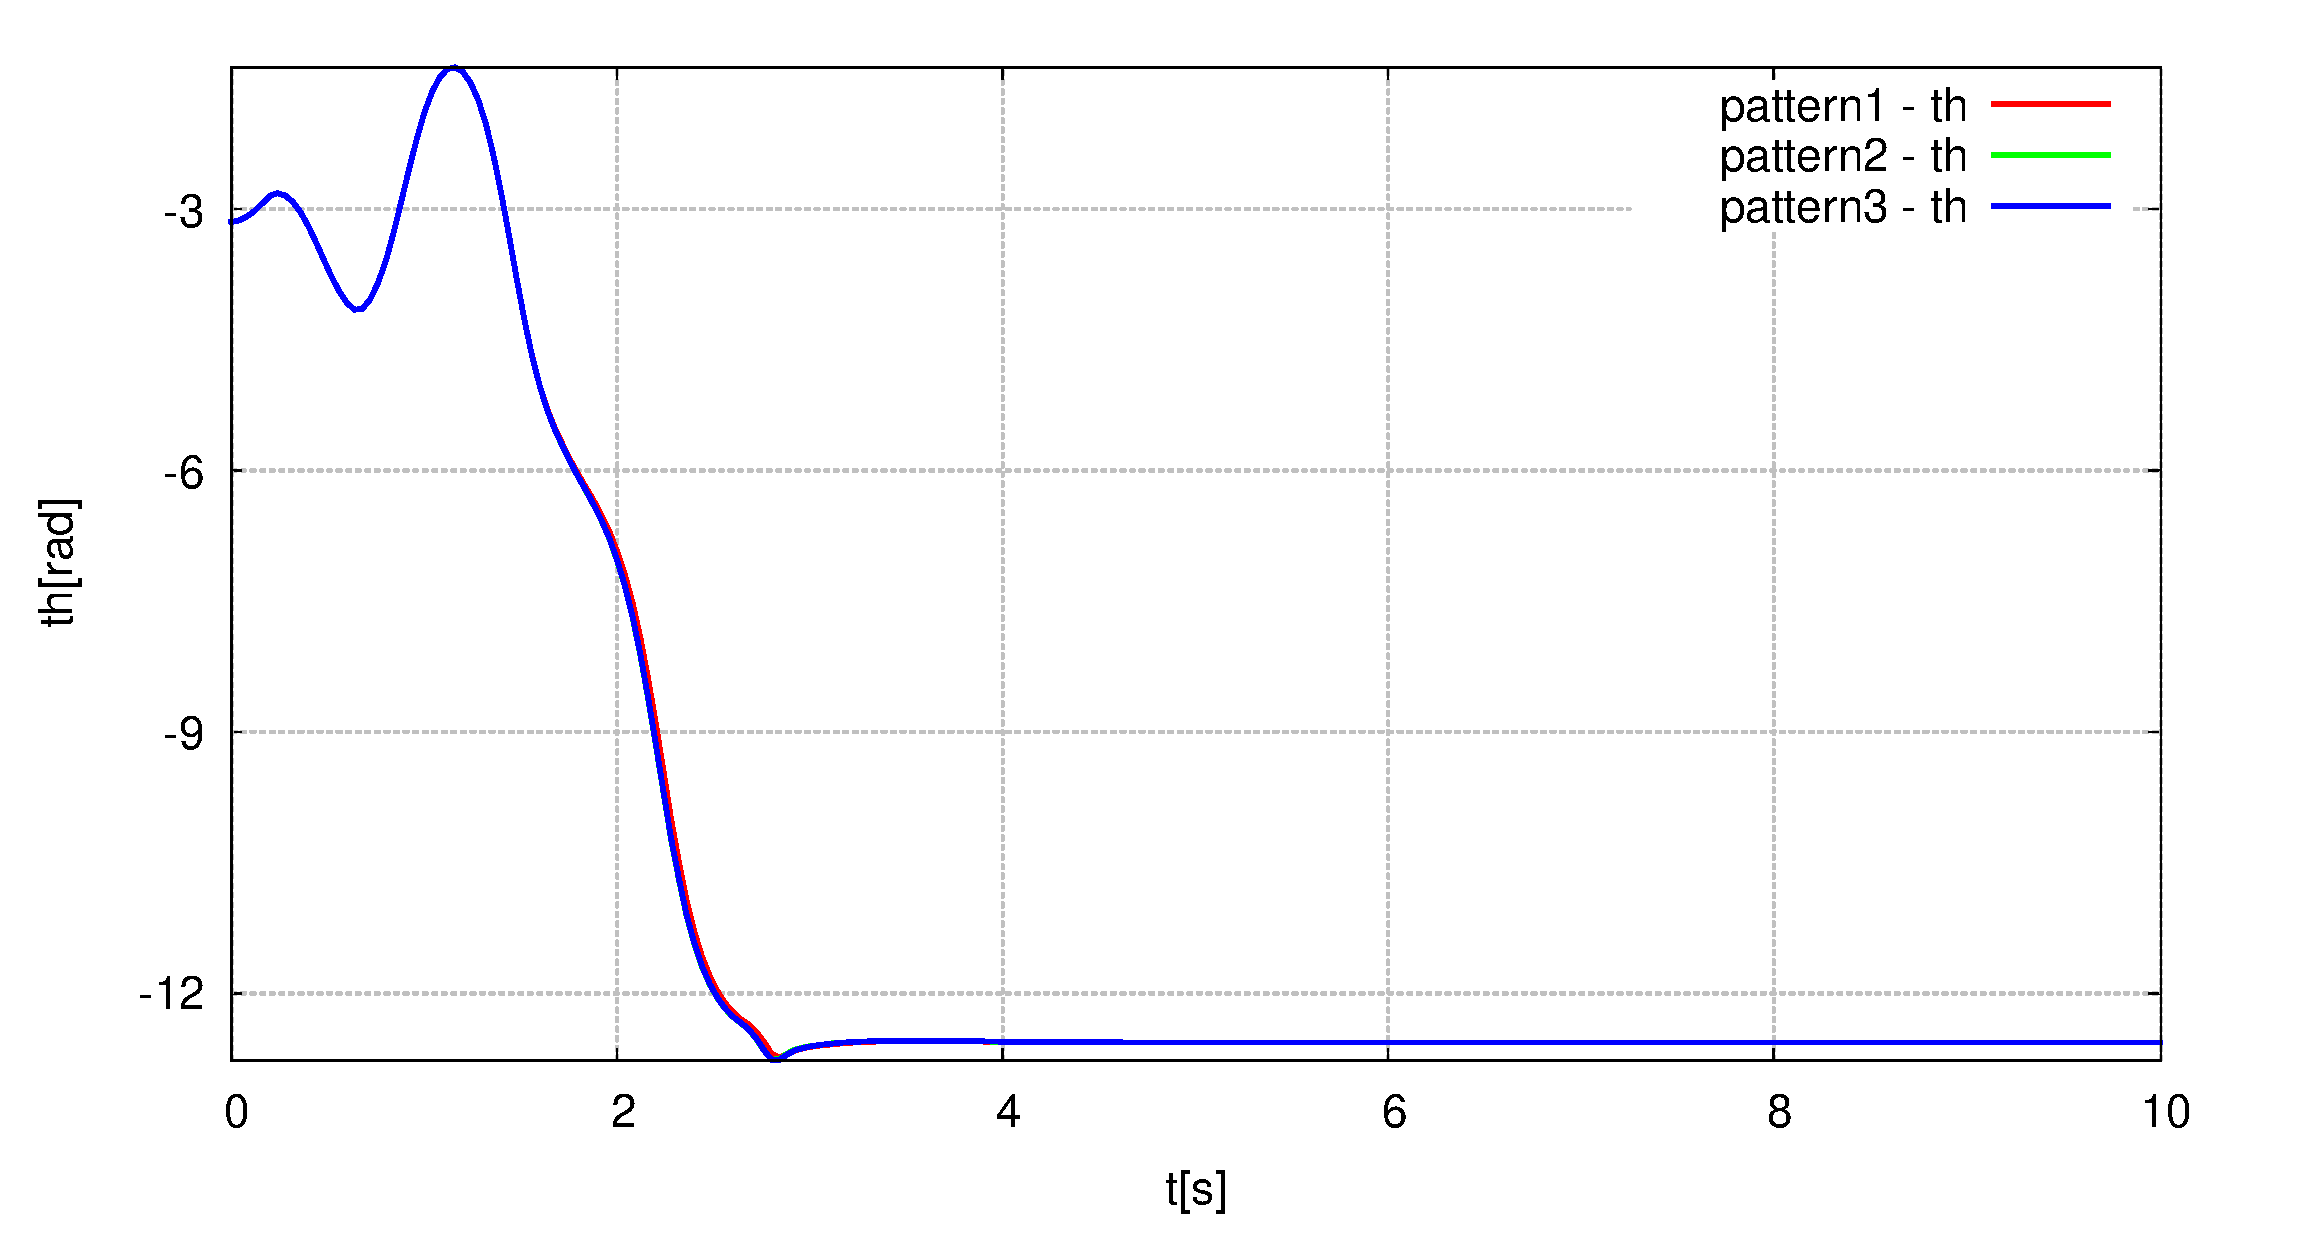
\includegraphics[width=0.4\linewidth]{gazo/Hsimu_TH.eps}
		\caption{振り上げ制御のシミュレーション比較結果}
		\label{image:simu_huriage}
	\end{figure}
	図\ref{image:simu_huriage}よりパラメータ$k$を変えても振り上げ制御から安定化制御に移行するまでの時間に変化がないことがわかる。
	前章のシステム解析においては$k$を大きくすると、エネルギーの収束が早くなると述べた。それにより、振り上げ制御にかかる時間は$k$を大きく
	することで短くなると予想したがそうではなかったようである。
	左図より、台車の位置に関しては$k$の値によって若干の差異が確認できるが、右図より、振子の角度に関しては$k$の値による差異はほとんど確認できない。
	以上から振り上げ制御に関して以下のことが言える。また、
	\begin{itemize}
	  \item $k$の値にかかわらず振り上げ制御から安定化制御に移行するまでの時間は一定である。
	  \item $k$の値にかかわらず安定化制御までの台車の位置と振子の角度はほぼ同じ挙動を示す。
	\end{itemize}
	ちなみに、右図より、振子の角度が$-12$より小さい値で収束していることから、このシミュレーションでは、
	振子は一回転半してから安定化制御に移ったと考えられる。
	
	
	
%--------------------------------------------------------------------------------------
\chapter{実験}
	\section{安定化制御実験}
\section{目標値の変更実験}
\section{振り上げ制御及び安定化実験}
\chapter{おわりに}
	本実験を通して当初の目的である、「倒立振子の安定化制御の制御系の設計を状態空間法を用いて行うことにより、線形時不変システムを設計すること」を達成できたといえる。
しかし、振り上げ実験においてはシミュレーションの結果と実験の結果に大きな差異が出てきてしまった。
そのため、実験を行う前と実験を行った後ではシミュレーションに対する評価が大きく変化した。
今後、シミュレーションを使用する機会があれば、そのシミュレーションの結果通りに実験結果が得られることはないことを
考慮した上で使用していきたい。
また、制御系のツールや数値計算ツールなどの使い方も習得することができた。
\chapter{まとめのーと(いずれ消してね)}
	\documentclass{jarticle}
\usepackage{amsmath}
\usepackage{ascmac}
\usepackage{fancybox}
\usepackage[dvipdfmx]{graphicx}
\usepackage{url}
\usepackage{color}
\begin{document}
	\begin{enumerate}
		{\LARGE\item\textgt{倒立振子のモデリングと自由応答シミュレーション}}\\
		\begin{enumerate}
			{\Large\item 倒立振子のモデリング}\\
			\begin{enumerate}
				{\large\item 実験テキスト等を参考にして倒立振子の運動方程式を(台車と振り子について)求める。}\\
					
					台車の運動方程式は\\
					\begin{equation}
						M\ddot{r}=au-F_{H}-f\dot{r}
					\end{equation}
					である。\\
					倒立振子の回転の運動方程式は\\
					\begin{equation}
						J\ddot{\theta}=lF_{V}\sin \theta -lF_{H}\cos \theta -c\dot{\theta}
					\end{equation}
					である。\\
					倒立振子の水平方向の運動方程式は\\
					\begin{equation}
						m\frac{d^{2}}{dt^{2}}(r+l\sin\theta) = F_{H}
					\end{equation}
					である。\\
					倒立振子の垂直方向の運動方程式は\\
					\begin{equation}
						m\frac{d^{2}}{dt^{2}}(l\cos\theta) = F_{V}-mg
					\end{equation}
					である。\\
					
				{\large\item 導出過程を記述}\\
				
					\begin{figure}[htbp]
						\begin{center}
							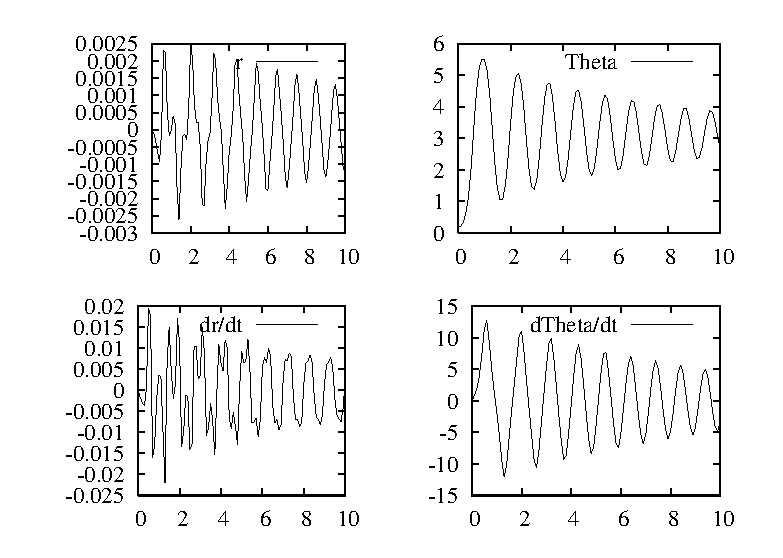
\includegraphics[width = 8cm]{gazo/InPeAboveNonLiner.eps}
						\end{center}
						\caption{台車にかかる力}
					\end{figure}
					図1より台車の運動方程式は、振り子からの水平抗力$F_{H}$を考慮してニュートンの第二法則より(1)式を導くことができる。\\
					ただし、$M$は台車の質量、$f$は台車の摩擦係数、$a$は駆動アンプへの入力電圧から台車への駆動までのゲイン、$u$はモータの駆動アンプへの入力電圧、$r$は台車の基準位置からの変位である。\\
					\\
					以下、同様にしてニュートンの第二法則を用いることで(3)、(4)式の運動方程式を導くことができる。図2を参考にするとよい\\
					\\
					\begin{figure}[htbp]
						\begin{center}
							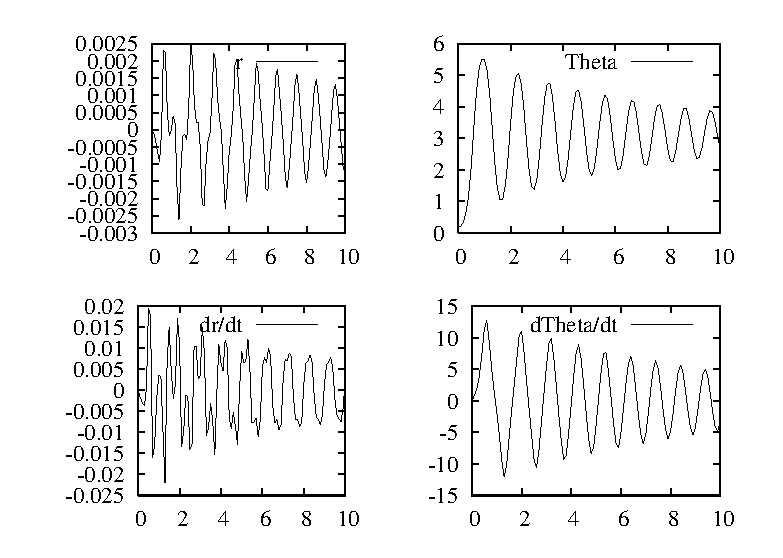
\includegraphics[width = 8cm]{gazo/InPeAboveNonLiner.eps}
						\end{center}
						\caption{振り子にかかる力}
					\end{figure}
					ただし、$m$は振り子の質量、$l$は回転軸・重心間の距離、$g$は重力加速度、$F_{V}$は振り子が台車から受ける垂直抗力である。
					また、$\theta$は鉛直上向きを$\theta=0$としたときの角度である。\\
					最後に(2)式は回転に対する運動方程式を考えることで上と同様に求めることができる。
					ただし、$J$は重心回りの慣性モーメント、$c$は回転軸摩擦係数である。\\
					
				{\large\item $x=\begin{pmatrix} r & \theta & \dot{r} & \dot{\theta} \end{pmatrix}^{\mathrm{T}}$ のように選び、(非線形モデル)非線形状態方程式$\dot{x}=f(x,u)$を導く。}\\
				
					いま、4つの状態変数から成るベクトル、すなわち状態$x$を\\
					
					\begin{eqnarray}
						x=\left[
						\begin{array}{ccc}
							r\\
							\theta\\
							\dot{r}\\
							\dot{\theta}\\
						\end{array}
						\right]
					\end{eqnarray}
					
					のように定義し、(1),(2),(3),(4)式から倒立振子系の非線形状態方程式を求める。\\
	
					\begin{eqnarray}
						\dot{x} = f(x,u) = \left[
						\begin{array}{ccc}
							\dot{r}\\
							\dot{\theta}\\
							\ddot{r}\\
							\ddot{\theta}\\
						\end{array}
						\right]
					\end{eqnarray}
					
					ここで(3)式より$F_{H}$を、(4)式より$F_{V}$を求めると\\
					
					\[F_{H} = m\frac{d^{2}}{dt^{2}}r + ml\frac{d^{2}}{dt^{2}}\sin{\theta}\]
					\begin{equation}
						    = m\ddot{r}+ml(-\dot{\theta}^{2}\sin{\theta}+\ddot{\theta}\cos{\theta})
					\end{equation}
					\\
					\[F_{V} = mg + m\frac{d^{2}}{dt^{2}}(l\cos{\theta})\]
					\begin{equation}
						= mg + ml(-\dot{\theta}^{2}\cos{\theta}-\ddot{\theta}\sin{\theta})
					\end{equation}
					\\
					(7)式を(1)式に代入すると\\
					\begin{equation}
						(M+m)\ddot{r} + ml\ddot{\theta}\cos{\theta}-ml\dot{\theta}^{2}\sin{\theta}+f\dot{r}=au
					\end{equation}
					\\
					(7)式、(8)式を(2)式に代入すると\\ TODO
					\begin{equation}
						(J + ml^{2})\ddot{\theta} + ml\ddot{r}\cos{\theta} - mgl\sin{\theta} + c\dot{\theta} = 0
					\end{equation}
					\\
					(9)式、(10)式を行列表現すると\\
					\begin{eqnarray}
						\left[
						\begin{array}{ccc}
							(M + m)\ddot{r} + (ml\cos{\theta})\ddot{\theta} + (-ml\sin{\theta}) + f\dot{r} = au \\
							(ml\cos{\theta})\ddot{r} + (J + ml^{2})\ddot{\theta} -mgl\sin{\theta} + c\dot{\theta} = 0\\
						\end{array}
						\right]
					\end{eqnarray}
					\begin{eqnarray}
						\left[
						\begin{array}{ccc}
							M + m & ml\cos{\theta} \\
							ml\cos{\theta} & J + ml^{2}\\
						\end{array}
						\right]
						\left[
						\begin{array}{ccc}
							\ddot{r} \\
							\ddot{\theta}\\
						\end{array}
						\right] +
						\left[
						\begin{array}{ccc}
							-ml\ddot{\theta}^{2}\sin{\theta} + f\dot{r}\\
							mgl\sin{\theta} + c\dot{\theta}\\
						\end{array}
						\right] = 
						\left[
						\begin{array}{ccc}
							au\\
							0\\
						\end{array}
						\right]
					\end{eqnarray}
					\\
					$\begin{pmatrix} M + m & ml\cos{\theta} \\ ml\cos{\theta} & J + ml^{2} \end{pmatrix}$を$K$と置いて右辺に逆行列としてかけると\\
					\begin{equation}
						\left[
						\begin{array}{ccc}
							\ddot{r}\\
							\ddot{\theta}\\
						\end{array}
						\right]=K^{-1}
						\left[
						\begin{array}{ccc}
							au-f\dot{r}+ml\ddot{\theta}\sin{\theta}\\
							mgl\sin{\theta} - c\dot{\theta}\\
						\end{array}
						\right]
					\end{equation}
					\\
					よって以上から(6)式は\\
					\begin{equation}
						\dot{x} = f(x,u)=\left[
						\begin{array}{ccc}
							\dot{r}\\
							\dot{\theta}\\
							K^{-1}\left[
							\begin{array}{ccc}
								-f\dot{r}+ml\ddot{\theta}\sin{\theta}+au\\
								mgl\sin{\theta}-c\dot{\theta}
							\end{array}
							\right]
						\end{array}
						\right]
					\end{equation}
					\\
					となる。ただし、$K$は
					\begin{equation}
					K=\left[
					\begin{array}{ccc}
						M+m & ml\cos{\theta}\\
						ml\cos{\theta} & J+ml^{2}\\
					\end{array}
					\right]
					\end{equation}
					\\
					である。
					\\
	
				{\large\item 平衡点$x=\begin{pmatrix} 0 & 0 & 0 & 0 \end{pmatrix}^{\mathrm{T}}$近傍で線形化し、(線形モデル)線形状態方程式$\dot{x}=Ax+Bu$と出力方程式$y=Cx$を導く。}\\	
				
					この時、この基準状態まわりで(15)式を一次近似することを考える。\\
					(15)式に一次近似のテイラー展開を施すと、\\
					\begin{equation}
						f(x,u) = f(0,0) + \left.\frac{\partial f}{\partial x}\right|_{x=0,u=0}(x-0) + \left.\frac{\partial f}{\partial u}\right|_{x=0,u=0}(u-0)
					\end{equation}
					\\
					となる。\\
					また、$A=\left.\frac{\partial f}{\partial x}\right|_{x=0,u=0} , B=\left.\frac{\partial f}{\partial u}\right|_{x=0,u=0}$とする。\\
					ここで、一時近似を施したので、$\theta$を微小範囲と考えることができ、$\sin{\theta} \simeq  \theta , \cos{\theta} \simeq 1 , \dot{\theta}^{2} \simeq 0$のように
					近似できる。\\
					以上の近似を(14)、(15)式に適用すると\\
					\begin{equation}
						f(x,u)=\left[
						\begin{array}{ccc}
							\dot{r}\\
							\dot{\theta}\\
							K^{'-1}\left[
							\begin{array}{ccc}
								au-f\dot{r}\\
								mlg\theta-c\dot{\theta}\\
							\end{array}
							\right]
						\end{array}
						\right]
					\end{equation}
					\begin{equation}
						K^{'} = \left[
						\begin{array}{ccc}
							M + m & ml\\
							ml & J+ml^{2}\\
						\end{array}
						\right]
					\end{equation}
					\\
					(17)、(18)式を用いてA、Bを計算する\\
					ここで、(17)式の3行目を$a_{1}$と置き、4行目を$a_{2}$と置く。\\
					\begin{equation}
						A=\frac{\partial \textgt{f}}{\partial \textgt{x}}=\\
						\left[
						\begin{array}{cccc}
							\frac{\partial \dot{r}}{\partial r} & \frac{\partial \dot{r}}{\partial \theta} & \frac{\partial \dot{r}}{\partial \dot{r}} & \frac{\partial \dot{r}}{\partial \dot{\theta}} \\
							\frac{\partial \dot{\theta}}{\partial r} & \frac{\partial \dot{\theta}}{\partial \theta} & \frac{\partial \dot{\theta}}{\partial \dot{r}} & \frac{\partial \dot{\theta}}{\partial \dot{\theta}} \\
							\frac{\partial a_{1}}{\partial r} & \frac{\partial a_{1}}{\partial \theta} & \frac{\partial a_{1}}{\partial \dot{r}} & \frac{\partial a_{1}}{\partial \dot{\theta}} \\
							\frac{\partial a_{2}}{\partial r} & \frac{\partial a_{2}}{\partial \theta} & \frac{\partial a_{2}}{\partial \dot{r}} & \frac{\partial a_{2}}{\partial \dot{\theta}} \\
						\end{array}
						\right]\\
					\end{equation}
					\begin{equation}
						=\left[
						\begin{array}{cccc}
							0 & 0 & 1 & 0 \\
							0 & 0 & 0 & 1 \\
							0 & 0 & K^{'-1}(-f) & 0\\
							0 & K^{'-1}(mgl) & 0 & K^{'-1}(-c) \\
						\end{array}
						\right]
					\end{equation}
					\\
					\begin{equation}
						B=\frac{\partial \textgt{f}}{\partial \textgt{u}}=
						\left[
						\begin{array}{c}
							\frac{\partial \dot{r}}{\partial u}\\
							\frac{\partial \dot{\theta}}{\partial u}\\
							\frac{\partial a_{1}}{\partial u}\\
							\frac{\partial a_{2}}{\partial u}\\
						\end{array}
						\right]=
						\left[
						\begin{array}{c}
							0\\
							0\\
							K^{'-1}a\\
							0\\
						\end{array}
						\right]
					\end{equation}
					\\
					よって線形状態方程式は\\
					\[\dot{x}=A\textgt{x}+B\textgt{u}\]
					\begin{equation}
						=\left[
						\begin{array}{cccc}
							0 & 0 & 1 & 0 \\
							0 & 0 & 0 & 1 \\
							0 & 0 & K^{'-1}(-f) & 0 \\
							0 & K^{'-1}(mgl) & 0 & K^{'-1}(-c)\\
						\end{array}
						\right]
						\left[
						\begin{array}{c}
							r\\
							\theta\\
							\dot{r}\\
							\dot{\theta}\\
						\end{array}
						\right] + 
						\left[
						\begin{array}{c}
							0\\
							0\\
							K^{'-1}au\\
							0\\
						\end{array}
						\right]
					\end{equation}
					\\
					また、出力方程式は2つの観測出力は
					\begin{equation}
						y_{1} = c_{1}r\\
					\end{equation}
					\begin{equation}
						y_{2} = c_{2}\theta\\
					\end{equation}
					のように表される。ここで、$c_{1}$は変位・電圧変換係数、$c_{2}$は角度・電圧変換係数である。これから成るベクトル出
					力$y$を\\
					\begin{equation}
						y=\left[
						\begin{array}{c}
							y_{1}\\
							y_{2}\\
						\end{array}
						\right]
					\end{equation}
					のように定義すると、倒立振子系に対する観測方程式として\\
					\begin{equation}
						y=Cx
					\end{equation}
					\begin{equation}
						\left[
						\begin{array}{c}
							y_{1}\\
							y_{2}\\
						\end{array}
						\right]=\left[
						\begin{array}{cccc}
							c_{1} & 0 & 0 & 0 \\
							0 & c_{2} & 0 & 0\\
						\end{array}
						\right]\left[
						\begin{array}{c}
							r\\
							\theta\\
							\dot{r}\\
							\dot{\theta}\\
						\end{array}
						\right]
					\end{equation}
					を得ることができる。\\
					
				
			\end{enumerate}
			{\Large\item 非線形モデルに基づく自由応答シミュレーション}\\
			\begin{enumerate}
				{\large\item 倒立振子の非線形モデルの状態の微分(ベクトル)
	 		   	$\dot{x}=\begin{bmatrix} \dot{r} & \dot{\theta} & \ddot{r} & \ddot{\theta} \end{bmatrix}^{\mathrm{T}}$
	 		   	を返す関数\textgt{diff\_eqs()}を書く。}\\
	 		   	
	 		   		以下に、MaTXで作成したdiff\_eqs()を以下に示す。\\
	 		   		\begin{itembox}[l]{diff\_eqs()}
	 		   			// diff\_eqs() は微分方程式を記述する関数\\
						Func void diff\_eqs(DX,t,X,UY)\\
						// tは時間\\
						Real t;\\
						Matrix X,DX,UY;\\
						\{\\
							Real M,m,l,J,f,a,c,g,r,th,dr,dth;\\
							Real xp2size;\\
							Matrix xp,up,dxp;\\
							Matrix K,KZ,CO,SI;\\
							Integer i;\\
							\\
							//物理パラメータの設定\\
							M=1.49;        m=0.038; l=0.13;\\
							J=4.5E-4; f=15.10; a=0.73;\\
							c=2.1E-4; g=9.8;\\
							\\
							//Xはx=(r Theta dr/dt dTheta/dt)\^Tを表す\\
							xp = X;\\
							// Uyは入力\\
							up = UY;\\
							\\
							r=X(1,1);\\
							th=X(2,1);\\
							dr=X(3,1);\\
							dth=X(4,1);\\
							\\
							K=[[M + m           , m * l * cos(th)  ]
							     [m * l * cos(th) , J + m * l * l    ]];
							\\
							KZ=[[    -f*dr      + m*l*sin(th)*dth*dth + a * up(1,1)]
								[ m*g*l*sin(th) - c*dth            ]];\\
							\\
							dxp=[[X(3:4,1)][K\textbackslash KZ]];\\
							DX \ = [dxp];\\
						\}\\
					\end{itembox}
					\\
	 		   	
				{\large\item 入力を0とし、真上から$(0^\circ~20^\circ)$傾けたところから離した場合のシミュレーションを実行する。シミュ
				レーションには関数Odeを用いる}\\
				
					以下にシミュレーションを行った出力結果を示す。\\
					左から$r , \theta , \dot{r} , \dot{\theta}$である。ただし、シミュレーションは10秒間行う。データ行が101個あるので、最
					初の0秒目のデータと最後の10秒目のデータを以下に示す。
					\begin{itembox}[l]{XC(出力結果)}
						\# 4 101\\
						0.00000000E+000  1.74532925E-001  0.00000000E+000  0.00000000E+000\\
						省略\\
						-1.20435914E-003  2.64681608E+000  2.46294987E-003 -3.33770438E+000\\
					\end{itembox}
				
				{\large\item 得られたデータをプロットする(mgplot利用)}\\
				
					以下にmgplotを用いてデータをプロットした結果を示す。\\
					\begin{figure}[htbp]
						\begin{center}
							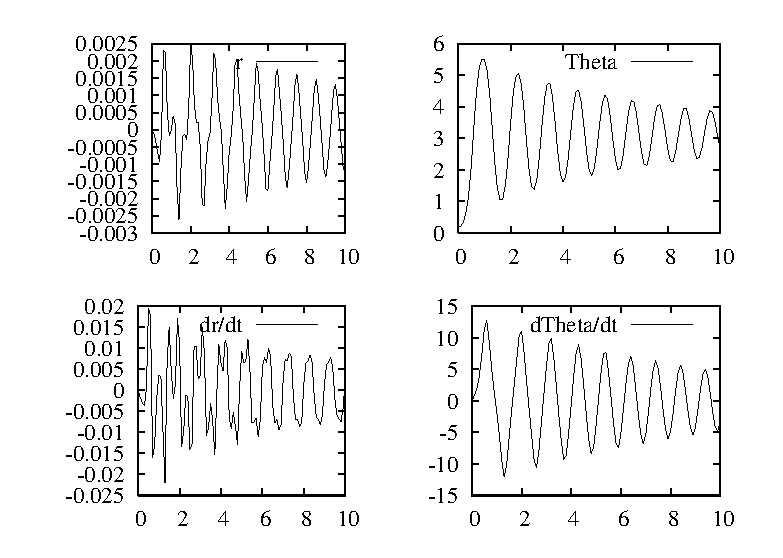
\includegraphics[width=8cm]{gazo/InPeAboveNonLiner.eps}\\
						\end{center}
						\caption{データのプロット結果}
					\end{figure}
					\\
				
				{\large\item グラフをEPSファイルに保存する。}\\
				
					上の図3はグラフをepsファイルに保存したものを貼り付けている。epsファイルを生成するために使用するコマンドはmgplot
					$\_$eps(1,''data.eps'')でファイルに保存することができる。\\
				
				{\large\item EPSファイルをPDFファイルに変換する}\\
				
					以下のウェブサイトにアクセスすることでEPSファイルをPDFファイルに変換することができる。\\
					\textcolor{cyan}{\url{https://convertio.co/ja/vector-converter/}}\\
					\\
					以下に変換したpdfファイルを示す。\\
					\begin{figure}[htbp]
						\begin{center}
							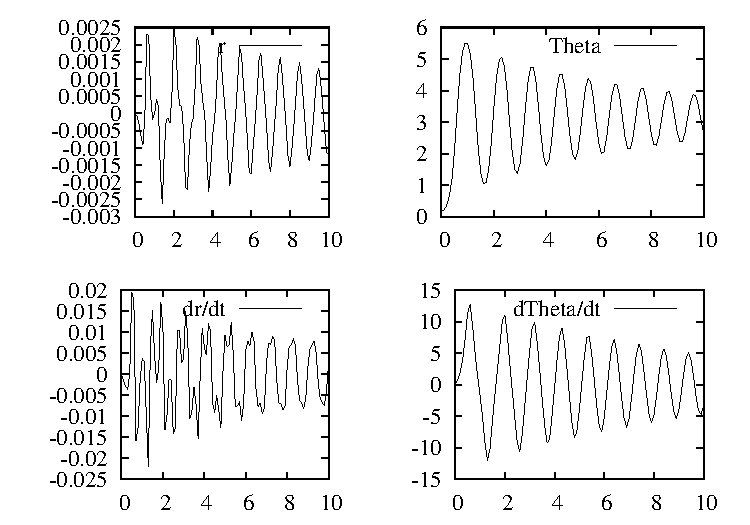
\includegraphics[width=8cm]{gazo/InPeAboveNonLiner.pdf}\\
						\end{center}
						\caption{EPSファイルをPDFに変換した結果}
					\end{figure}
				
				{\large\item グラフをプリンタに出力する}\\
				
					上で変換したPDFファイルを印刷した。\\
				
				{\large\item 関数Odeの代わりにOde45やOde45Autoを用い、結果を比較する}\\
				
				まず、Odeで計算した結果とOde45で計算した結果を比較する。以下にOdeで計算した場合とOde45で計算した場合を一緒
				のグラフにプロットした図を示す。\\
				\begin{figure}[htbp]
					\begin{center}
						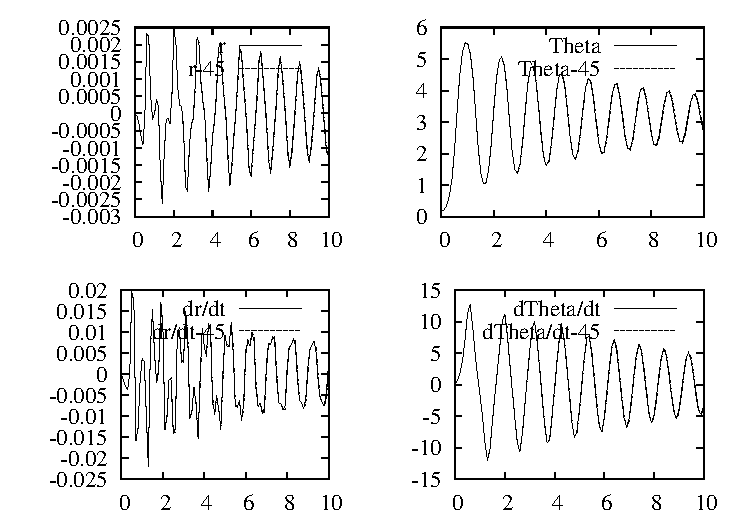
\includegraphics[width=8cm]{gazo/OdeOde45Comp.pdf}\\
					\end{center}
					\caption{Odeを使用した場合とOde45を使用した場合の比較}
				\end{figure}
				\\
				関数Odeは微分方程式をルンゲ・クッタ法で求める方法であり関数Ode45は微分方程式をRunge-Kutta-Fehlberg(RKF45)
				で求める方法である。つまり、両関数は微分方程式の解法が異なるだけである。図5からは両関数における大きな違いを確認
				することはできない。\\
				次にOdeで計算した結果とOde45Autoで計算した結果を比較する。以下にOdeで計算した場合とOde45Autoで計算した場合
				を一緒にのグラフにプロットした図を示す。
				\begin{figure}[htbp]
					\begin{center}
						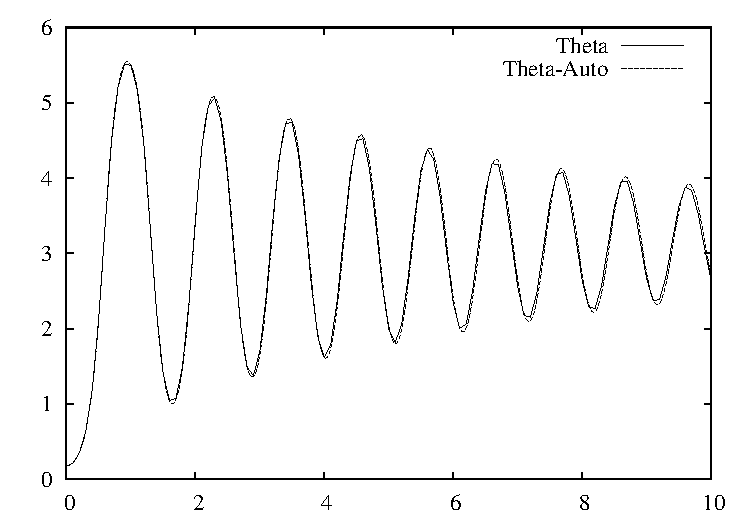
\includegraphics[width=8cm]{gazo/OdeOde45AutoComp.pdf}\\
					\end{center}
					\caption{Odeを使用した場合とOde45Autoを使用した場合の比較}
				\end{figure}
				\\
				Ode45Autoを用いることで変化が急なところの描画がより滑らかになっていることが確認できる。Ode45Autoは応答の緩急に応じ
				て刻み幅を自動で調整してくれる関数である。\\
				
				
			\end{enumerate}
			{\Large\item 線形モデルに基づくシミュレーションおよび非線形モデルとの比較}\\
			\begin{enumerate}
				{\large\item 倒立振子の非線形モデルと線形モデルの自由応答を比較する}\\
				
					最初に線形モデルのdiff$\_$eqs()を以下に示す。\\
					\begin{itembox}[l]{diff\_eqs()}
						// diff\_eqs() は微分方程式を記述する関数\\
						Func void diff\_eqs(DX,t,X,UY)\\
						// tは時間\\
						Real t;\\
						Matrix X,DX,UY;\\
						\{\\
							Real M,m,l,J,f,a,c,g;\\
							Matrix xp,up,dxp;\\\
							Matrix A,B,A21,A22,B2,K;\\
						\\
							//物理パラメータの設定\\
							M=1.49;        m=0.038; l=0.13;\\
							J=4.5E-4; f=15.10; a=0.73;\\
							c=2.1E-4; g=9.8;\\
							\\
							K=[[M+m,m*l][m*l,J+m*l\^2]];\\
							A21 = K~*[[0,0][0,m*g*l]];	\\
							A22 = K~*[[-f,0][0,-c]];\\
							A=[[Z(2),I(2)][A21,A22]];\\
							\\
							B2 = K~*[[a][0]];\\
							B=[[Z(2,1)][B2]];\\
							\\
							//Xはx=(r Theta dr/dt dTheta/dt)\^Tを表す\\
							xp = X;\\
							// Uyは入力\\
							up = UY;\\
							\\
							dxp = A*xp+B*up;\\
							\\
							DX = [dxp];\\
							\\
						\}\\
					\end{itembox}
					\\
					以下に上の線形モデルを用いて出力したデータのプロットと非線形モデルを用いて出力したデータのプロットを比較した図を
					示す。\\
					\begin{figure}[htbp]
					\begin{center}
						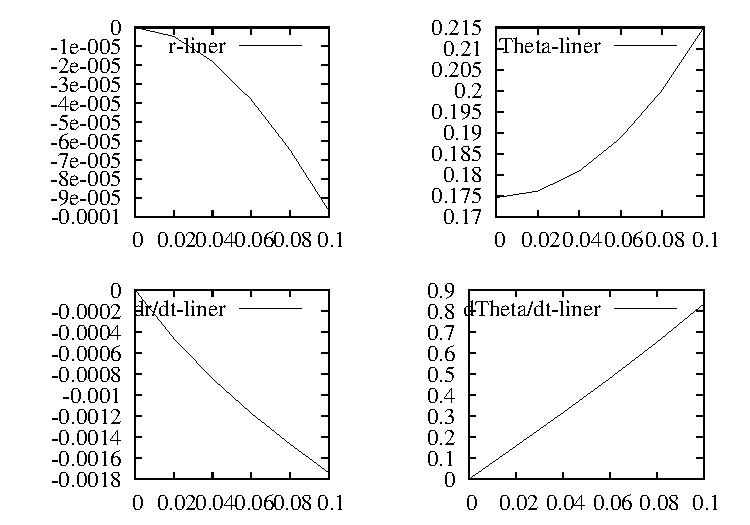
\includegraphics[width=8cm]{gazo/InPeAboveLiner.pdf}\\
					\end{center}
					\caption{線形モデルの出力データ}
					\end{figure}
					\begin{figure}[htbp]
					\begin{center}
						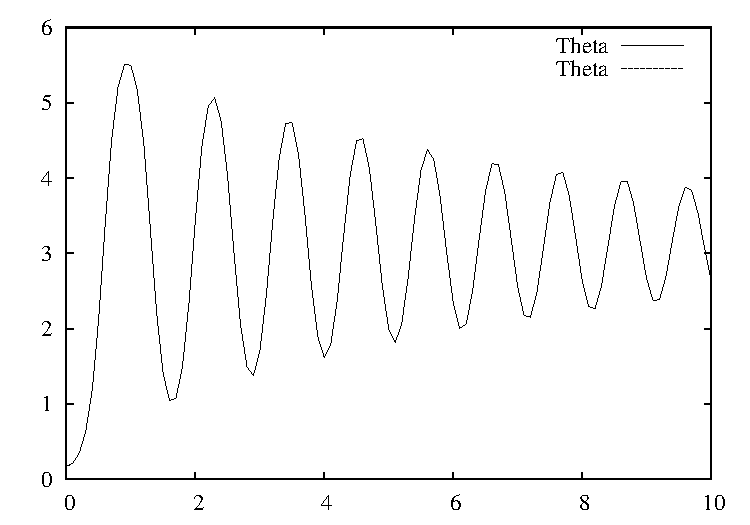
\includegraphics[width=8cm]{gazo/AboveLinerNonLinerComp.pdf}\\
					\end{center}
					\caption{線形モデルと非線形モデルの比較}
					\end{figure}
					\\
					図8はほとんど非線形モデルのグラフしか見えないが、線形モデルは0秒付近においてのみ描画されている。\\
					図7からこの線形モデルの応答が発散していることがわかる。つまり、この線形モデルではうまくいかないことがわかる。\\
				
				{\large\item 時間が進むにつれ、応答がますます離れていくのはなぜか?安定性について調べよ}\\
				
					$\theta$を微小範囲内で考えたためである。振子を上から$10^{゜}$ずらして手を離した場合、振子は真っ逆さまにおいて
					いき、$\theta$は大きくなり、前提としている$\theta$を微小範囲内という条件を満たさなくなってしまう。このような平衡点を
					不安定平衡点という。また、固有値を調べてその実部を見ることでそのモデルの安定性を調べることができる。今回の振子が上
					向き線形モデルの固有値$\lambda$はMaTXのeigval関数を用いると\\
					\begin{equation}
						\lambda = \left[
						\begin{array}{c}
							0\\
							0\\
							0.87\\
							-4.3\\
						\end{array}
						\right]
					\end{equation}
					となった。このときすべての極の実部が負でないので安定でないことがわかる。\\
					
				
				{\large\item 振り子の角度を鉛直下向を$\theta=0$として、状態方程式を求める}\\
				
					このとき、	(14)、(15)式は振子が上向きであるときを$\theta=0$として設定している。ここでは、振子が下向きであるときを
					$\theta=0$として設定しているので、(14),(15)式の三角関数内の$\theta$に+$\pi$すれば求めたい状態方程式を導くこ
					とができるといえる。なので、振り子の角度を鉛直下向きを$\theta=0$としたときの状態方程式は\\
					\begin{equation}
						\dot{x} = f(x,u)=\left[
						\begin{array}{ccc}
							\dot{r}\\
							\dot{\theta}\\
							K^{-1}\left[
							\begin{array}{ccc}
								-f\dot{r}-ml\ddot{\theta}\sin{\theta}+au\\
								-mgl\sin{\theta}-c\dot{\theta}
							\end{array}
							\right]
						\end{array}
						\right]
					\end{equation}
					\\
					となる。ただし、$K$は
					\begin{equation}
					K=\left[
					\begin{array}{ccc}
						M+m & -ml\cos{\theta}\\
						-ml\cos{\theta} & J+ml^{2}\\
					\end{array}
					\right]
					\end{equation}
				
				{\large\item 平衡点$x=\begin{pmatrix} 0 & 0 & 0 & 0 \end{pmatrix}^{\mathrm{T}}$近傍で線形化し、(線形モデル)線形
				状態方程式$\dot{x}=Ax+Bu$と出力方程式$y=Cx$を導く。}\\
				
					振子の角度を鉛直上向きを$\theta=0$としたときの状態方程式を線形化したときと同様に(29),(30)式を線形化すると
					線形状態方程式は\\
					\[\dot{x}=A\textgt{x}+B\textgt{u}\]
					\begin{equation}
						=\left[
						\begin{array}{cccc}
							0 & 0 & 1 & 0 \\
							0 & 0 & 0 & 1 \\
							0 & 0 & K^{'-1}(-f) & 0 \\
							0 & K^{'-1}(-mgl) & 0 & K^{'-1}(-c)\\
						\end{array}
						\right]
						\left[
						\begin{array}{c}
							r\\
							\theta\\
							\dot{r}\\
							\dot{\theta}\\
						\end{array}
						\right] + 
						\left[
						\begin{array}{c}
							0\\
							0\\
							K^{'-1}au\\
							0\\
						\end{array}
						\right]
					\end{equation}
					\\
					となる。ただし、$K$は、
					\begin{equation}
					K=\left[
					\begin{array}{ccc}
						M+m & -ml\\
						-ml & J+ml^{2}\\
					\end{array}
					\right]
					\end{equation}
					である。\\
					また、線形出力方程式は(27)式と同様である。\\
					今後、倒立振子のシミュレーションや検証を行う際のモデルは(31),(32)式を用いる。\\
				
				{\large\item 入力を0とし、真下から$(0^\circ~20^\circ)$傾けたところから離した場合の線形モデルと非線形モデルの応答を
				比較する}\\
				
					以下に真下から$10^\circ$傾けたところから離した場合の線形モデルと非線形モデルの$\theta$の応答を比較した図を
					示す。\\
					\begin{figure}[htbp]
						\begin{center}
							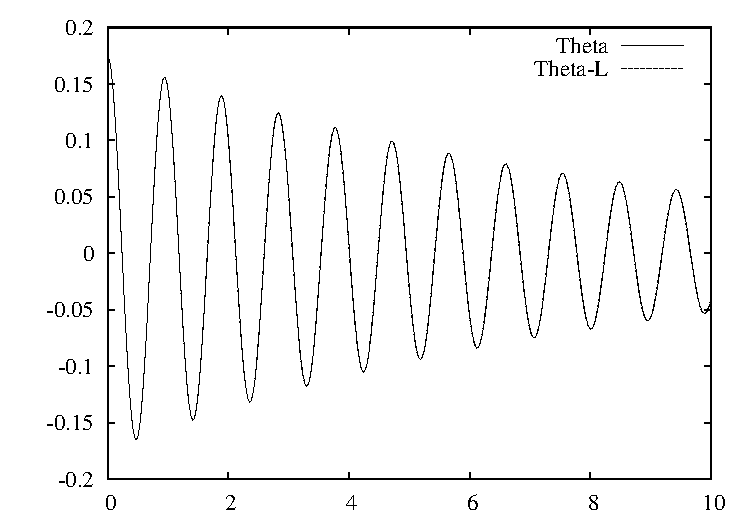
\includegraphics[width=8cm]{gazo/UnderLinerCompTheta.pdf}\\
						\end{center}
						\caption{線形モデルと非線形モデルの応答比較}
					\end{figure}
					図9から線形モデルと非線形モデルの応答がほぼ一致していることがわかる。真上の角度を$\theta=0$としたときの線形モデルの
					応答と違い発散していないことがわかる。これは真下から$10^\circ$傾けたところで$\theta$が微小範囲から大きくなることがな
					いためである。このときの平衡点を安定平衡点という。以下の節で行うパラメータの同定、検証においてはこの線形モデルを使用
					しても問題ないことになる。\\
				
			\end{enumerate}
			{\Large\item Java(NFC)によるモデリングとシミュレーション}\\
			\begin{enumerate}
				{\large\item 準備}\\
				
				nfcとwheelsをeclipseにインストールした\\
				倒立振子のシミュレーションを実行するプロジェクトを作成した\\
				その他準備を行った上で以下の作業を行う準備がそろっている。\\
				
				{\large\item モデリングとシミュレーション}\\
				
				ここでは、先ほど終了した準備をもとにjavaを用いてシミュレーションをモデリングを行う。上で線形モデルを用いると述べたがここでは
				非線形モデルをJAVAファイルに記述することでシミュレーションを行う。\\
				シミュレーションは倒立振子システムを表すPendulumクラスとシミュレーション対象システムを生成するFreePendulumクラスとシミュレー
				ションを実行するFreePendulumSimulationクラスによって行う。以下にシミュレーションを行ってgnuplotに描画した結果を以下に示
				す。ちなみにシミュレーションは鉛直下向きを$\theta=0$として行う\\
				\begin{figure}[htbp]
					\begin{center}
						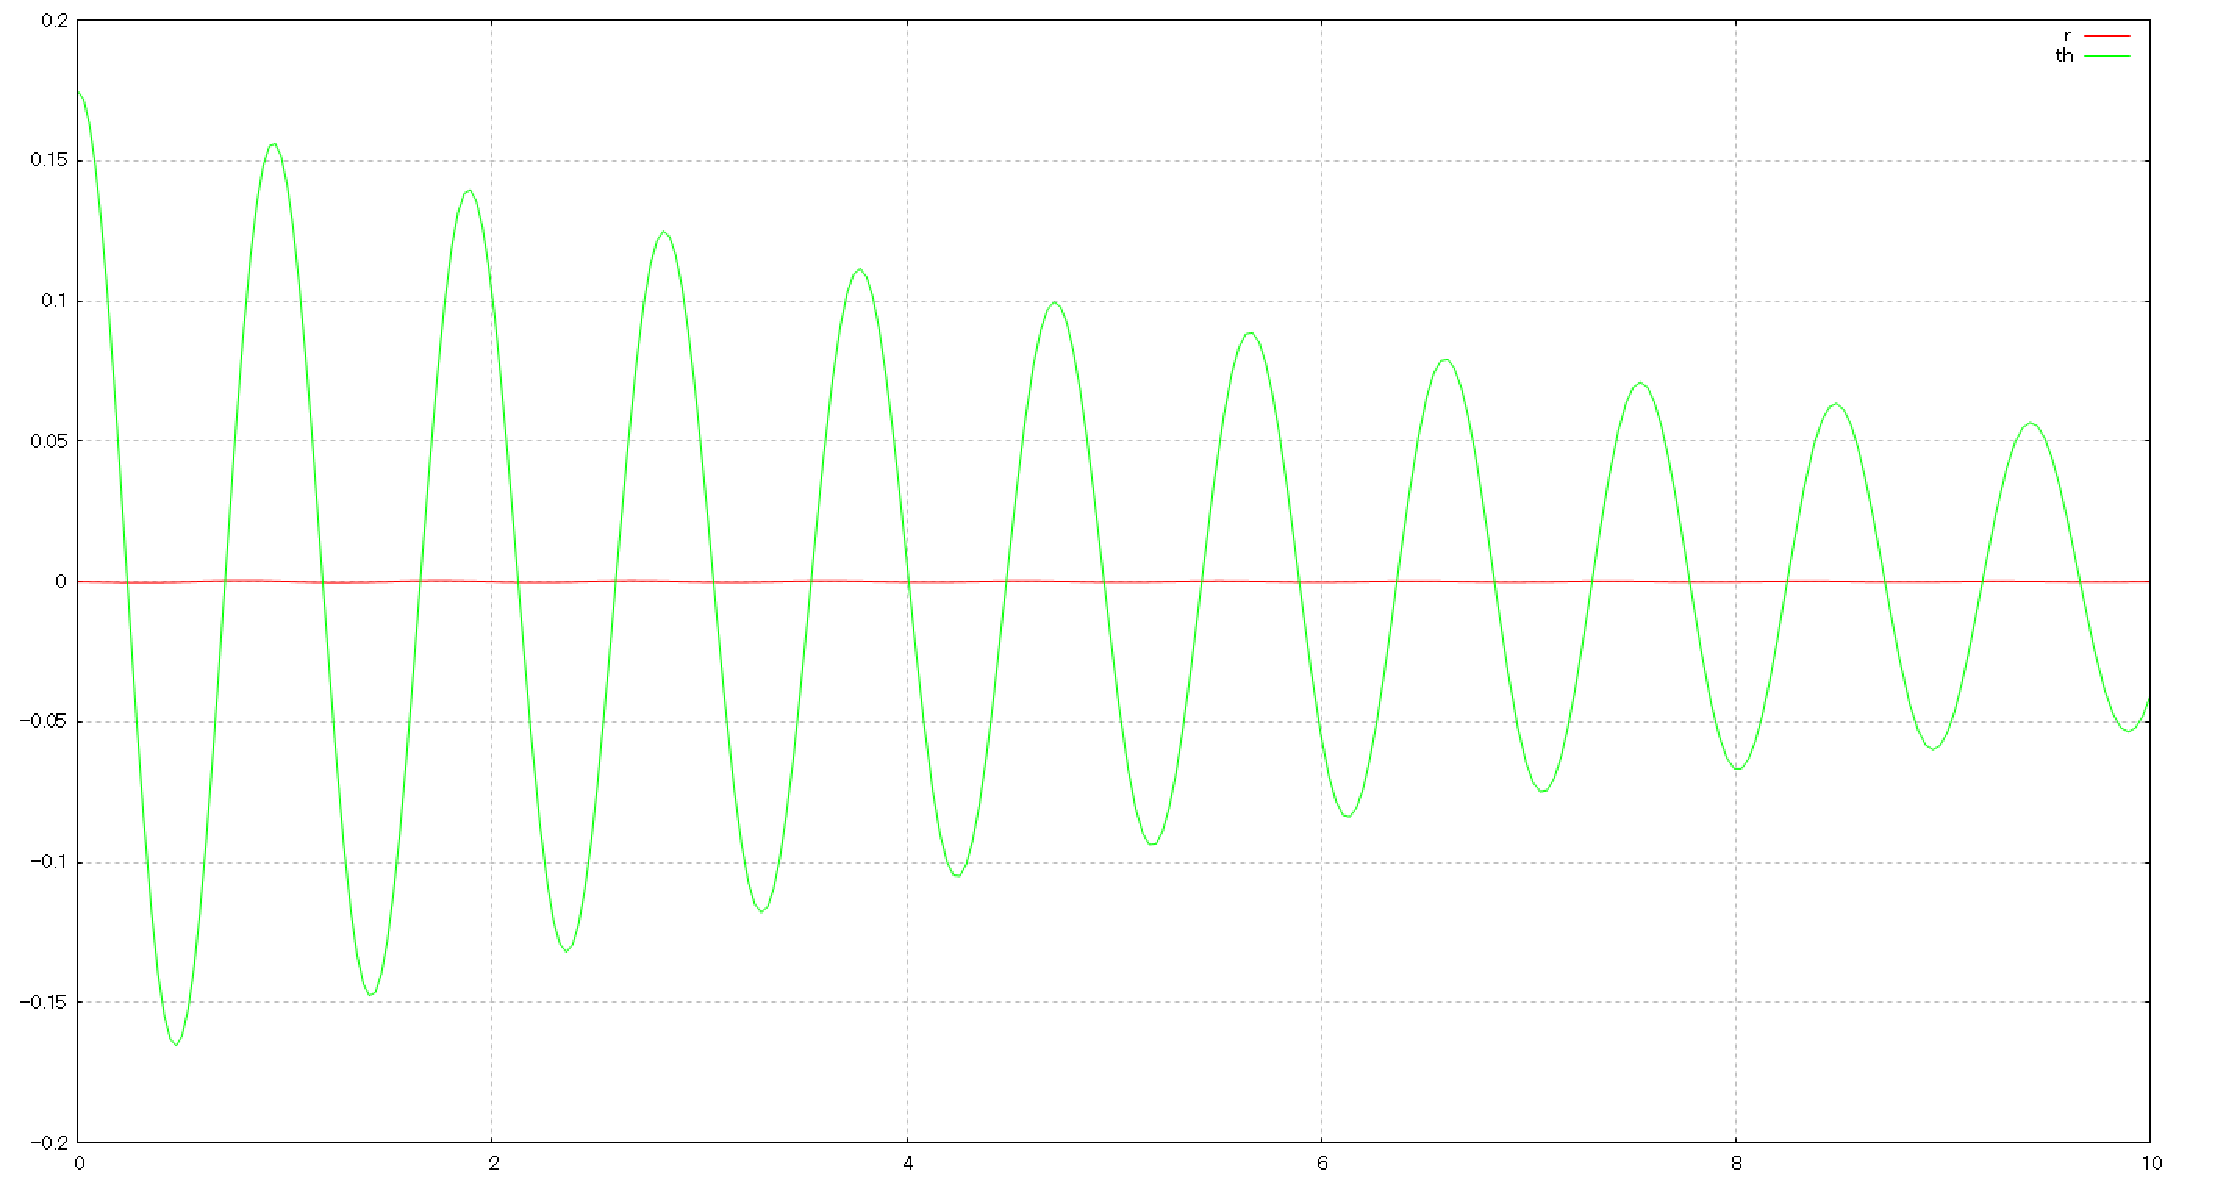
\includegraphics[width=8cm]{gazo/FreePendulumSimulationJAVAThetaR.pdf}\\
					\end{center}
					\caption{JAVAによるシミュレーション($\theta$を表示)}
				\end{figure}
				\begin{figure}[htbp]
					\begin{center}
						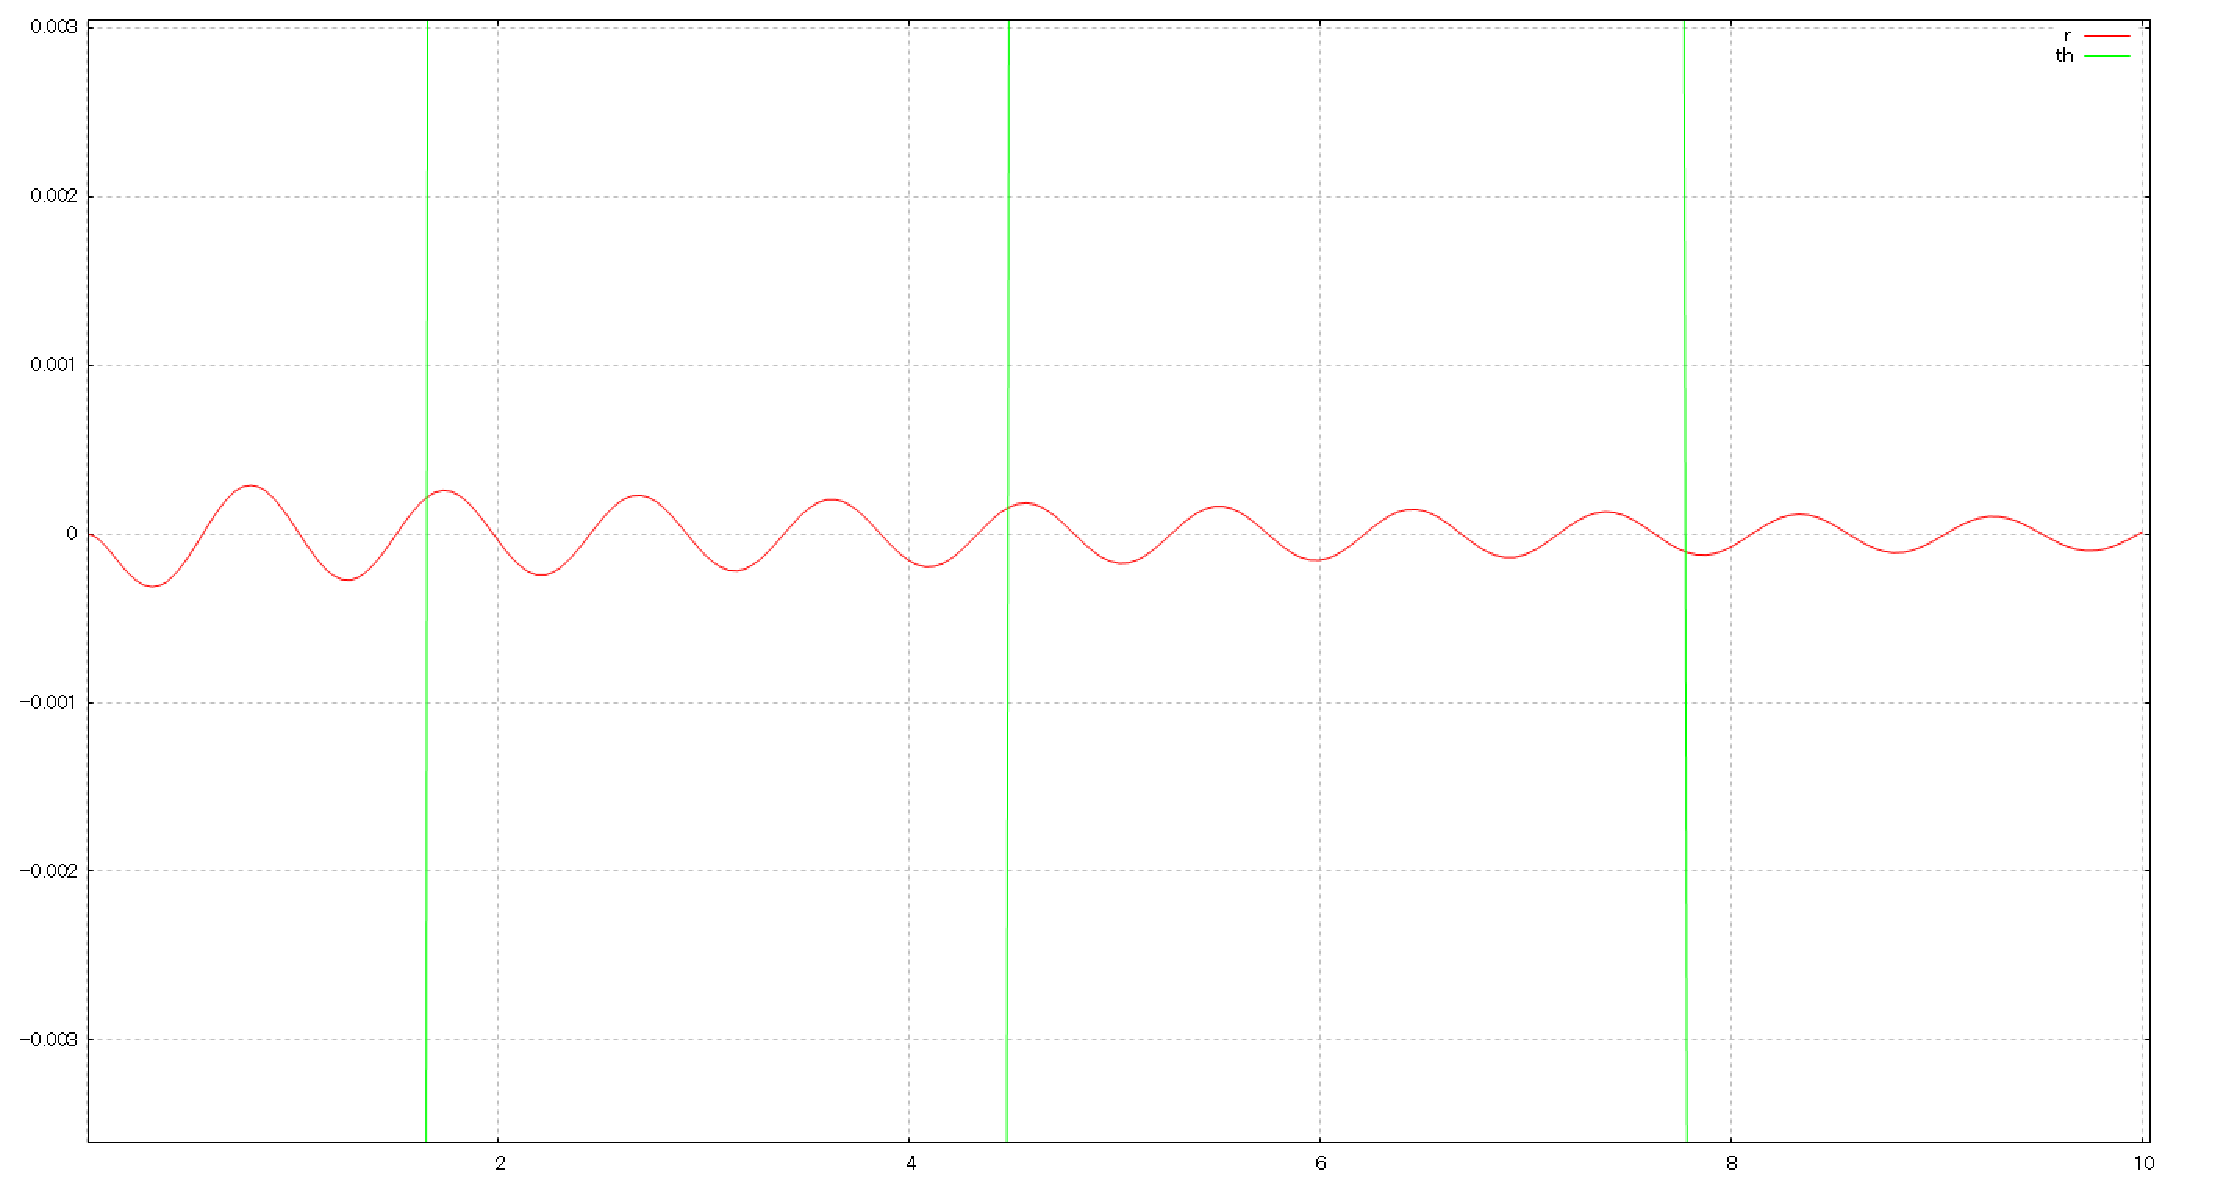
\includegraphics[width=8cm]{gazo/FreePendulumSimulationJAVAr.pdf}\\
					\end{center}
					\caption{JAVAによるシミュレーション($r$を表示)}
				\end{figure}
				
			\end{enumerate}
			{\Large\item Jamoxによるモデリングとシミュレーション}\\
			\begin{enumerate}
				{\large\item ユーザ定義動的システム(Java)による倒立振子システム}\\
				
					先ほど作成した倒立振子を表すPendulumクラスを用いて、JAMOXでシミュレーションを行う。\\
					以下に倒立振子のシミュレーションモデル(ブロック線図)と自由応答を示す。\\
					\begin{figure}[htbp]
					\begin{center}
						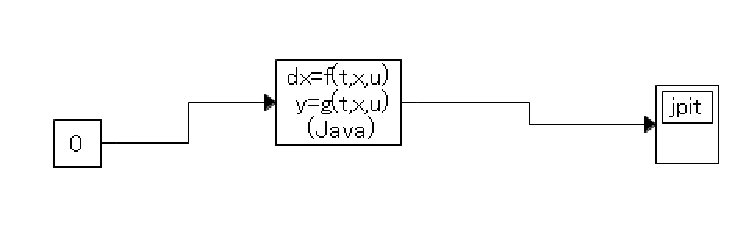
\includegraphics[width=8cm]{gazo/BlockNonLinerJ.pdf}\\
					\end{center}
					\caption{使用したブロック線図}
					\end{figure}
					\begin{figure}[htbp]
					\begin{center}
						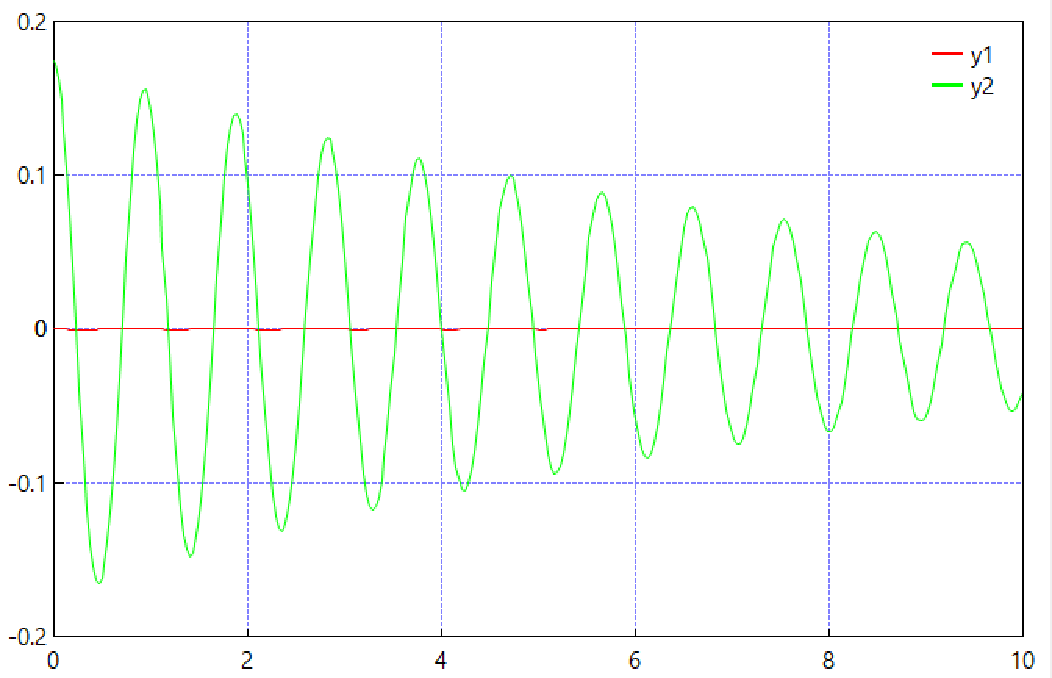
\includegraphics[width=8cm]{gazo/FreePendulumSimulationJAMOXJ.pdf}\\
					\end{center}
					\caption{自由応答波形}
					\end{figure}
				
				
				{\large\item ユーザ定義動的システム(MaTX)による倒立振子システム}\\
					
					今度はMaTXを用いて同様のシミュレーションを行う。以下に倒立振子のシミュレーションモデル(ブロック線図)と自由応答波形
					を示す。\\
					\begin{figure}[htbp]
					\begin{center}
						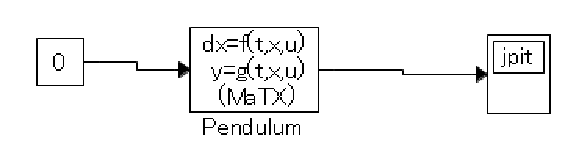
\includegraphics[width=8cm]{gazo/BlockNonLinerM.pdf}\\
					\end{center}
					\caption{使用したブロック線図}
					\end{figure}
					\begin{figure}[htbp]
					\begin{center}
						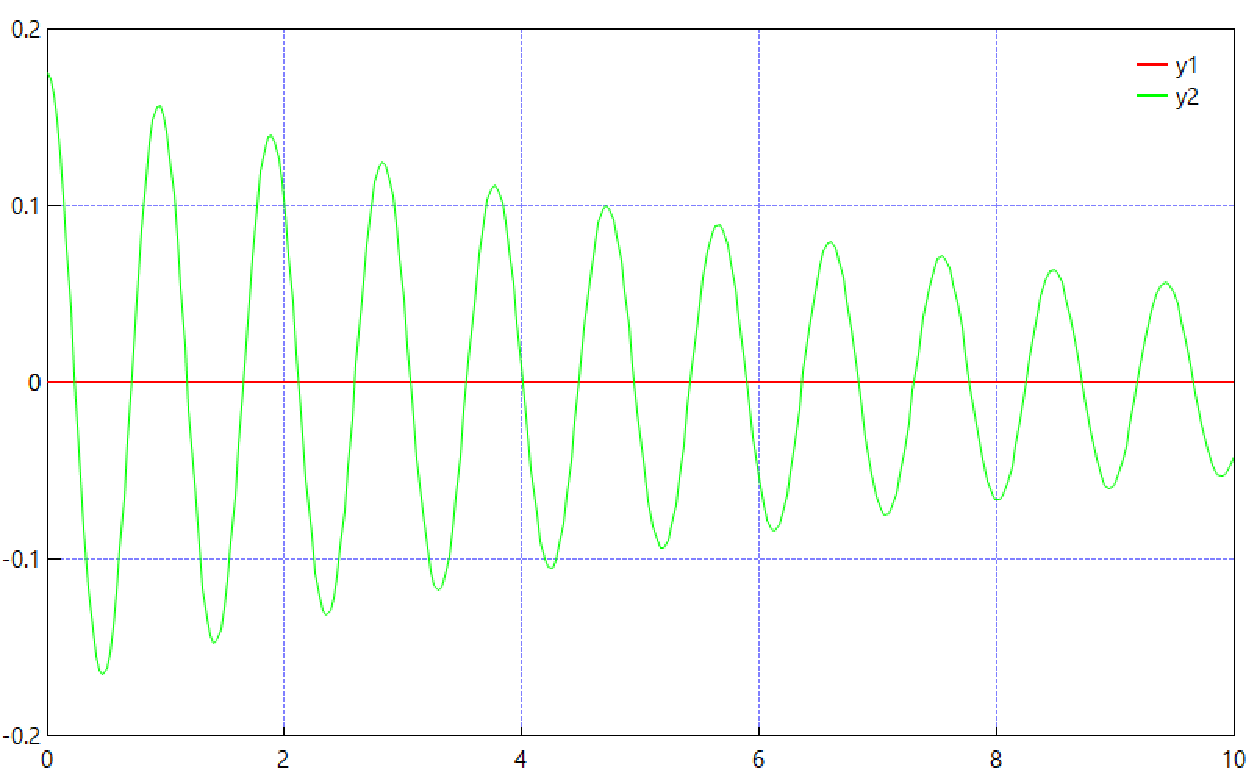
\includegraphics[width=8cm]{gazo/FreePendulumSimulationJAMOXM.pdf}\\
					\end{center}
					\caption{自由応答波形}
					\end{figure}
				
			\end{enumerate}
		\end{enumerate}	

		{\LARGE\item \textgt{倒立振子のパラメータ同定と検証}}\\ 
		\begin{enumerate}
			{\Large\item 実験環境(Linux2.6 + RtMaTX)の整備と確認}\\
			\begin{enumerate}
				{\large\item 実験方法}\\
				
					実験は実験室のPCと倒立振子を使う。PCで倒立振子の計測を行うには、ディレクトリRtMaTX内に存在するSample.mmファイ
					ルを用いる。Sample.mmをコンパイルするにはシェル内でmakeと打ち、Sample.mmを実行するには sudo ./sampleと入力すれば
					よい。実行した後は$\theta$とプログラム開始時を初期値として$r$の測定画面が現れる。cを押すことで台車に入力値が入
					り、測定が開始される。\\
					
				{\large\item sample.mmの解読}\\
				
					適宜必要な時に行えばよいかと。とりあえず入力を変えたいときはオンライン関数内のactuator()の引数を変えればよい。それ以
					上の情報はここでは\\
				
			\end{enumerate}
			{\Large\item パラメータの同定}\\
			\begin{enumerate}
				{\large\item 振り子の質量mの同定}\\
				
					振り子は台車から取り外した棒の部分を振り子として扱う。つまり、台車と振り子をつなぐための直方体の物体は台車の一部と
					して扱うことにする。同定は計量器を用いた。ここで計量器の精度が有効数字二桁までしかないので以後同定したパラメータも
					有効数字二桁で扱う。以下に同定した結果を示す。
					\begin{equation}
						m=3.1E-2(kg)
					\end{equation}
				
				{\large\item 振り子の回転軸から重心までの長さlの同定}\\
				
					先ほどと同様の振り子に対して重心までの長さを同定する。(見た感じ)振り子が左右対称であることを利用して振り子のちょう
					ど真ん中の位置を定規で測定した。以下に同定した結果を示す。
					\begin{equation}
						l=1.5E-1(m)
					\end{equation}
				
				{\large\item 変位rの測定値への変換係数$c_{1}$の同定}\\
				
					最初から設定してある。
					\begin{equation}
						c_{1}=1.0(V/m)
					\end{equation}
				
				{\large\item 角度$\theta$の測定値への変換係数$c_{2}$の同定}\\
				
					最初から設定してある。
					\begin{equation}
						c_{2}=1.0(V/m)
					\end{equation}
				
				{\large\item 駆動アンプへの入力電圧から台車への駆動力までのゲインaの同定}\\
				
					詳しい同定方法は資料の方を参考にしてもらいたい。ここでは、簡単に説明する。まず台車を左の方に位置させて台車を駆動
					させる。この時台車にばねばかりをひっかけ2パターンの状況においてその値を測定する。まずは台車をばねばかりでぎりぎり動か
					ない力で引っぱった場合、次に台車をばねばかりで逆に左に動き出す力で引っ張った場合、の2パターン値を入力電圧を変えな
					がら測定していく。そして、各パターンにおいて最小二乗法を用いて一時関数を求める。この傾きをaとする。以下に同定した値
					を示す。
					\begin{equation}
						a=0.062(Kg/V) = 6.1E-1(N/V)
					\end{equation}
				
				{\large\item 重心まわりの慣性モーメントJの同定}\\
				
					振り子を自由振動させることにより、Jとcを測定できる。詳しい数式は資料を参考されたい。ここでは簡単に説明する。振り子を
					自由振動させたときのデータからグラフを描画させる。グラフにおいて一つ目の山とその次の山から減衰比を求める。また、一つ目
					の山から次の山までにかかる時間を1周期として求める。この値を利用してJとcを求める。以下にJを求めるのに使用した数式を
					示す。
					\begin{equation}
						J=\frac{mglT_{2}^{2}}{4\pi^{2}+\lambda^{2}}-ml^{2}
					\end{equation}
					(38)式よりJは以下のように同定された。
					\begin{equation}
						J=2.5E-4(khm^{2})
					\end{equation}
				
				{\large\item 回転軸摩擦係数cの同定}\\
				
					上の通りである。以下にcを求めるのに使用した数式を示す。
					\begin{equation}
						c=\frac{2\lambda(J+ml^{2})}{T_{2}}
					\end{equation}
					(40)式よりcは以下のように同定された。
					\begin{equation}
						c=5.4E-5(kgm^{2}/s)
					\end{equation}
				
				{\large\item 台車の質量Mの同定}\\
				\begin{enumerate}
					{\item ステップ応答による方法}\\
					
						振り子を台車から取り外して、台車のステップ応答を測定する。詳しい数式は資料に譲る。各電圧についてステップ応答を							測定し、グラフを描画する。そのグラフから傾きKU0とその傾きを持つ一次関数を仮定したとき$r(t)=0$となるtをTとして決定							する。KとTからMとfを決定する。以下に同定したMを示す。
						\begin{equation}
							M=6.9E-1(kg)
						\end{equation}
						
					{\item フィードバックによる方法}\\
					
						振り子を台車から取り外すのは同じ。入力がステップ応答ではなくフィードバックになるのでそこを考慮する必要がある。
						つまり、sample.mmにおいてactuator()の引数を
						\[u=k_{c}*(y_{c}-y)\]
						という風に変更しなければならない。これができれば台車は目標値に向かってフィードバックし始める。\\
						得られたデータ列をプロットし、減衰比とその周期(Jとcの同定で用いた方法と同じ)を求める。
						求めたJとcから以下の式を用いて$\zeta$と$\omega_{n}$を計算し求める。
						\begin{equation}
							\lambda=\frac{2\pi\zeta}{\sqrt{1-\zeta^{2}}}
						\end{equation}
						\begin{equation}
							T_{2}=\frac{2\pi}{\omega_{n}\sqrt{1-\zeta^{2}}}
						\end{equation}
						上の式を式変形して$\zeta$と$\omega_{n}$イコールの式にすると
						\begin{equation}
							\zeta=\frac{\lambda}{\sqrt{4\pi^{2}+\lambda^{2}}}
						\end{equation}
						\begin{equation}
							\omega_{n}=\frac{2\pi}{T_{2}\sqrt{1-\zeta^{2}}}
						\end{equation}
						以上の式から求めた$\zeta$と$\omega_{n}$は以下の二次系の伝達関数の基本形に代入することで
						実験で得られたデータから伝達関数を求めることができる
						\begin{equation}
							G(s) = \frac{\omega_{n}^{2}}{s^{2}+2\zeta\omega_{n}s + \omega_{n}^{2}}
						\end{equation}
						また、今回のフィードバック制御系におけるブロック線図は以下のようになる。
						\begin{figure}[htbp]
						\begin{center}
							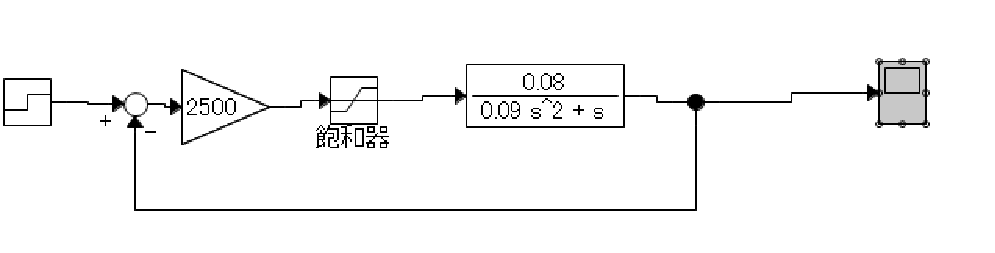
\includegraphics[width=8cm]{gazo/FeedBackCart.pdf}\\
						\end{center}
						\caption{フィードバック制御系のブロック線図}
						\end{figure}
						ここで、台車の伝達関数は以下の式である。
						\begin{equation}
							P(s)=\frac{K}{s(Ts+1)}
						\end{equation}
						ただし、Tは$M/f$、Kは$a/f$である。上のブロック線図から伝達関数を求める。
						しかし、飽和システムを含んでいると伝達関数を求めることができないので、ここでは飽和システムがなくても
						台車は問題なく動作するもとして仮定する。以上の仮定から伝達関数は
						\begin{equation}
							G(s) = \frac{AK/T}{s^{2}+(1/T)s+(AK/T)}
						\end{equation}
						となる。ただしAはゲインである。(47)式と(49)式を係数比較し、M、f=の式にすると以下のようになる。
						\begin{equation}
							\left\{
							\begin{array}{l}
								M=\frac{aA}{\omega_{n}^{2}} \\
								f=2\zeta\omega_{n}^{2}M
							\end{array}
							\right.
						\end{equation}
						よって、(50)式からMとfは以下のように求まる。
						\begin{equation}
						\left\{
						\begin{array}{l}
							M=1.59(kg)\\
							f=13.2(kg/s)
						\end{array}
						\right.
						\end{equation}
											
					{\item 2つの方法で求めたパラメータを比較する。パラメータが異な場合、その理由を考察する。}\\
					
						(42),(52)式と(51)式を比べるとまるで違うことがわかる。
						考察:結論から述べると飽和システムを無視しても問題なく動作すると仮定してパラメータを計算したためである。\\
						飽和システムを無視したことによる差異が生まれる\\
						飽和システムは飽和システムに設定した以上の電圧が入ったときにそのオーバーした分をカットする
						つまり飽和システムを無視することによりカットするかしないかで差異が生まれる
						実際に飽和システムにかかる前の電圧をシミュレーションとしてJAMOXか何かで見てみるといいが収束値0.2でゲイン250
						のとき一番最初に入力される電圧はなんと500Vである。これがどのくらいの電圧なのか専門家でないので知る余地もないが
						これを15Vとみなすかみなさないかで大きく差異が生まれるといえるだろう。画像は各自でそろえてほしい。mendoi
						なら飽和システムを含めて伝達関数を求めればよいのではないか?\\
						→飽和システムを含んでいるブロック線図の伝達関数は求めることができない(線形システムでないため)\\
						なら飽和システムに設定した以上の電圧が入らないように収束値、ゲインを調整すればよいのではない?\\
						→0.2に収束させるという条件で15Vを超えないゲインはだいたい70に設定すればよい。\\
 						だがこれではツェータが1を超えてしまいオーバーシュートしなくなる。つまりゲイン操作によって15V以内に入力を抑えるこ
 						とは不可能\\
						→ゲイン1500という設定で15Vを超えないような収束値は0.01である。つまり台車を1cmだけ動かすことになる。
						ハード的な問題から収束値1cmで正確なデータが取れるとは思えない\\

						つまり、以上から本実験においてフィードバックを行う場合必ず飽和システムが必要であるといえる。
						なので、飽和システムが存在する限り伝達関数を求めることができないので、正確なパラメータの計算を行うことができないと
						いえる。
						考察終わりん子
					
				\end{enumerate}
				{\large\item 台車の摩擦係数fの同定}\\
				
					上に示した通りである。ただし、ここではステップ応答による方法のみ取り扱う。以下に同定した値を示す。
					\begin{equation}
						f=7.6(kg/s)
					\end{equation}
				
				{\large\item パラメータを表にまとめる}\\
				
					同定実験において同定したパラメータを表にまとめる。\\
					\\
					\begin{tabular}{|c|c|}\hline
						パラメータ & 同定した値 \\ \hline\hline
						m[kg]  & 0.031\\ \hline
						l[m] & 0.15\\ \hline
						M[kg] & 0.69\\ \hline
						f[kg/s] & 7.56\\ \hline
						J[$kgm^{2}$] & 2.5E-4\\ \hline
						c[$kgm^{2}/s$] & 5.4E-5\\ \hline
						a[N/V] & 0.61\\ \hline
						$c_{1}$[V/m] & 1.0\\ \hline
						$c_{2}$[V/m] & 1.0\\ \hline
					\end{tabular}
					
				
			\end{enumerate}
			{\Large\item パラメータの検証}\\
			\begin{enumerate}
				{\large\item 台車のステップ応答}\\
				\begin{enumerate}
					{\item MaTXによる}\\
					
						以下に実験データとシミュレーション結果を重ね合わせたグラフを示す。ただし、入力電圧を8Vのときである。
						\begin{figure}[htbp]
						\begin{center}
							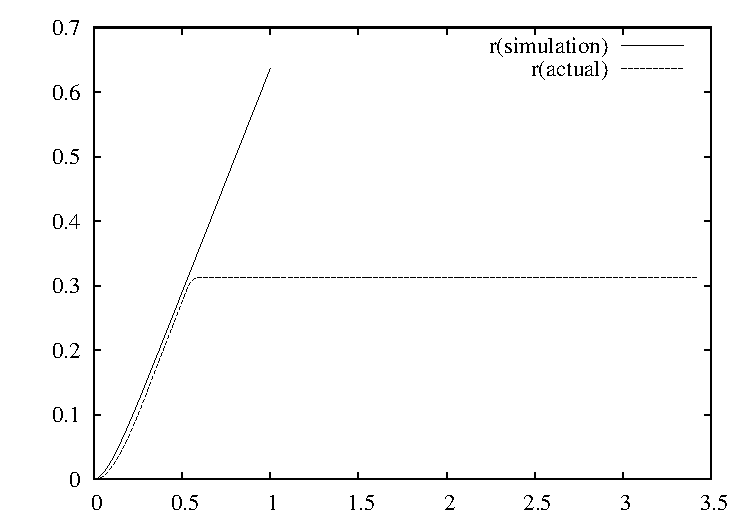
\includegraphics[width=8cm]{gazo/nabe8.pdf}\\
						\end{center}
						\caption{ステップ応答の実験データとシミュレーション結果のグラフ(MaTX)}
						\end{figure}
						
					{\item Javaによる}\\
					
						以下にjavaを用いて実験データとシミュレーション結果を重ね合わせたグラフを示す。ただし、入力電圧は8Vである。
						\begin{figure}[htbp]
						\begin{center}
							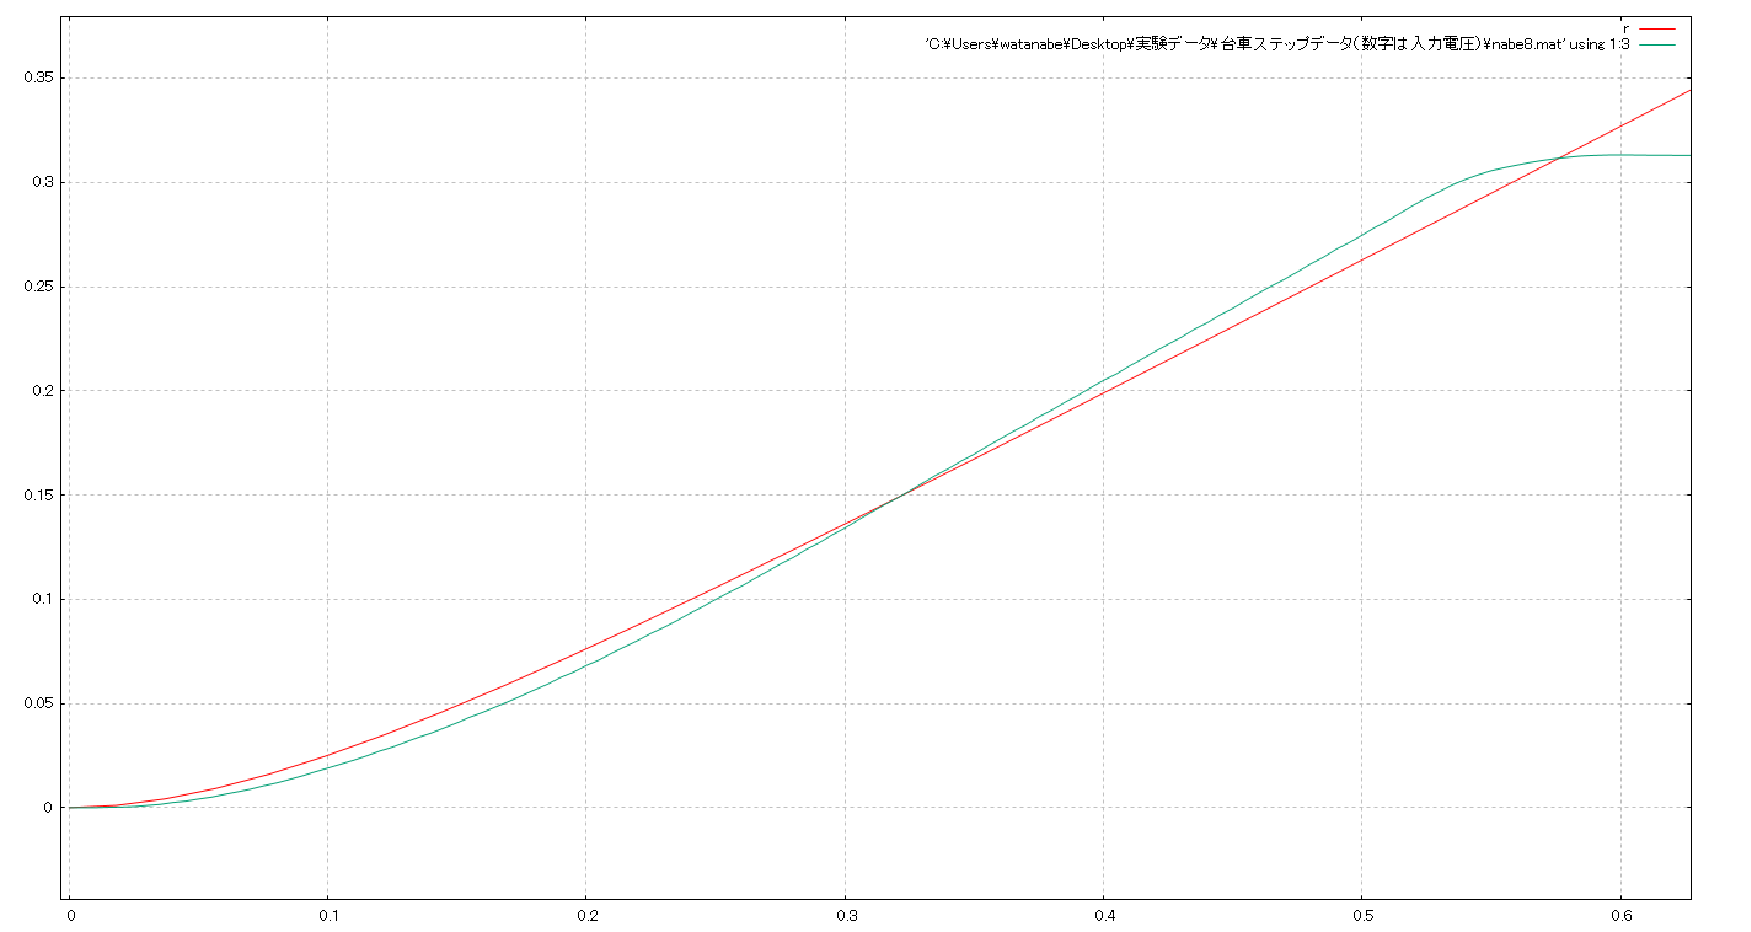
\includegraphics[width=8cm]{gazo/nabe8StepJAVA.pdf}\\
						\end{center}
						\caption{ステップ応答の実験データとシミュレーション結果のグラフ(JAVA)}
						\end{figure}
					
					{\item Jamoxによる}\\
					
						以下にJAMOXを用いて実験データをシミュレーション結果を重ねたグラフを示す。ただし、入力電圧は8Vである。
						ブロック線図は省略する。
						以下にユーザー定義関数システムJAVAを用いて検証した結果を示す。
						\begin{figure}[htbp]
						\begin{center}
							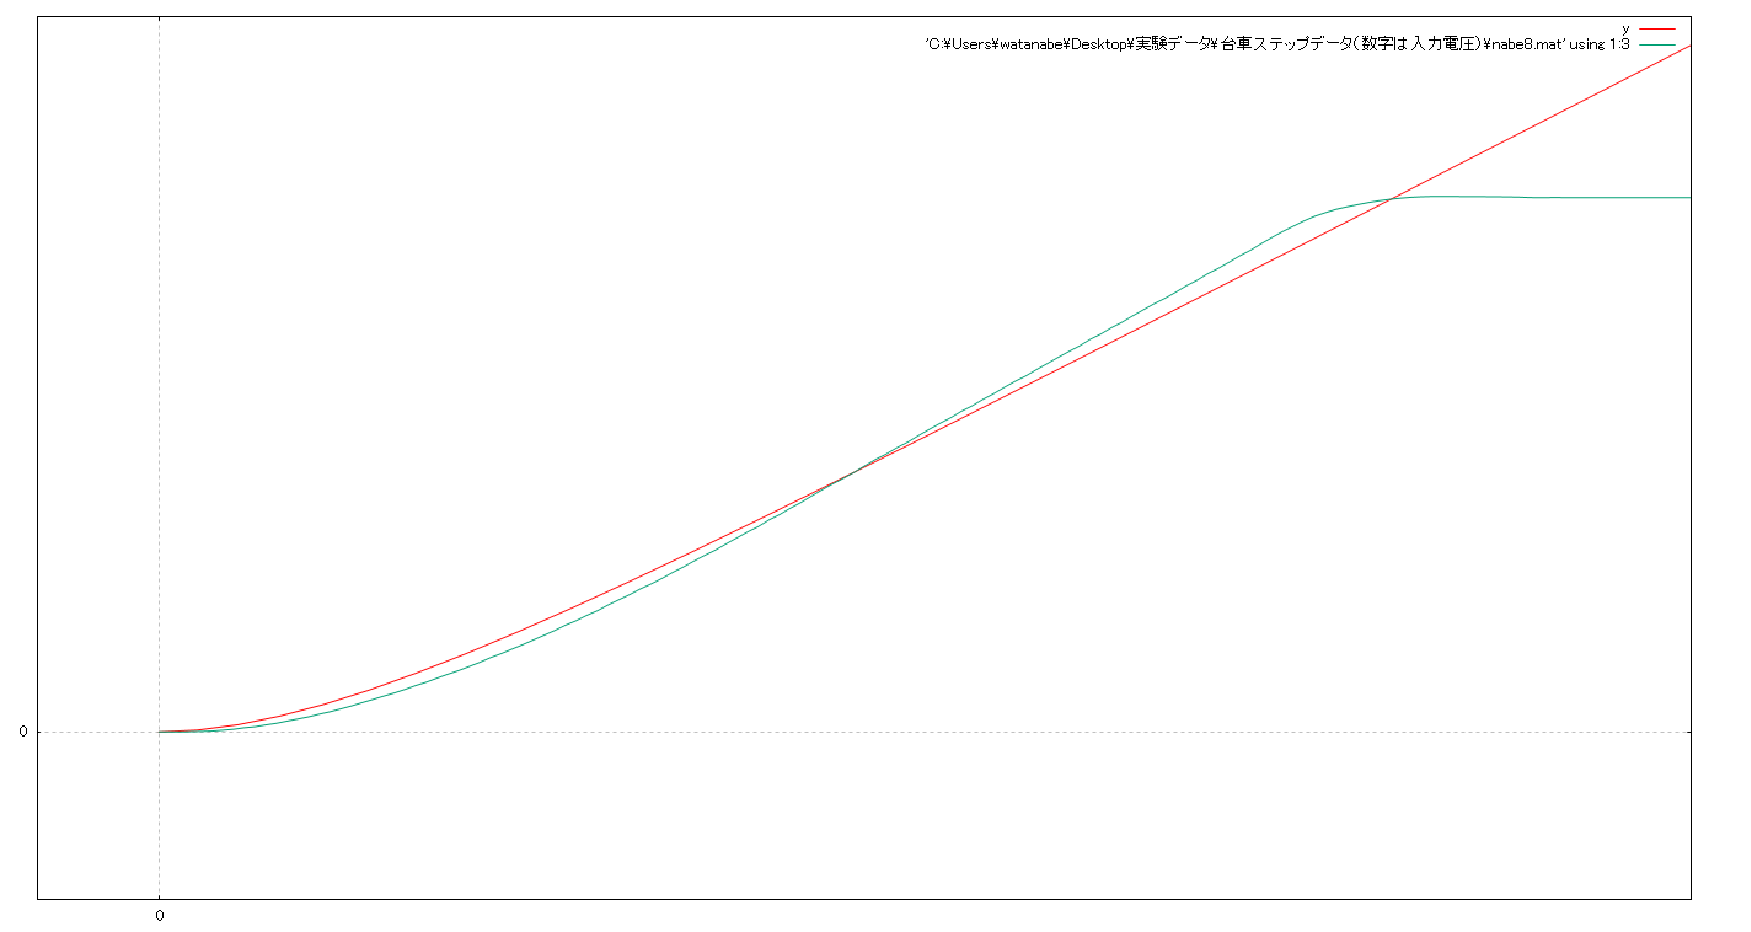
\includegraphics[width=8cm]{gazo/StepCartJAMOXJ.pdf}\\
						\end{center}
						\caption{ステップ応答の実験データとシミュレーション結果のグラフ(JAMOX(JAVA))}
						\end{figure}
						以下にユーザー定義関数システムMATXを用いて検証した結果を示す。
						\begin{figure}[htbp]
						\begin{center}
							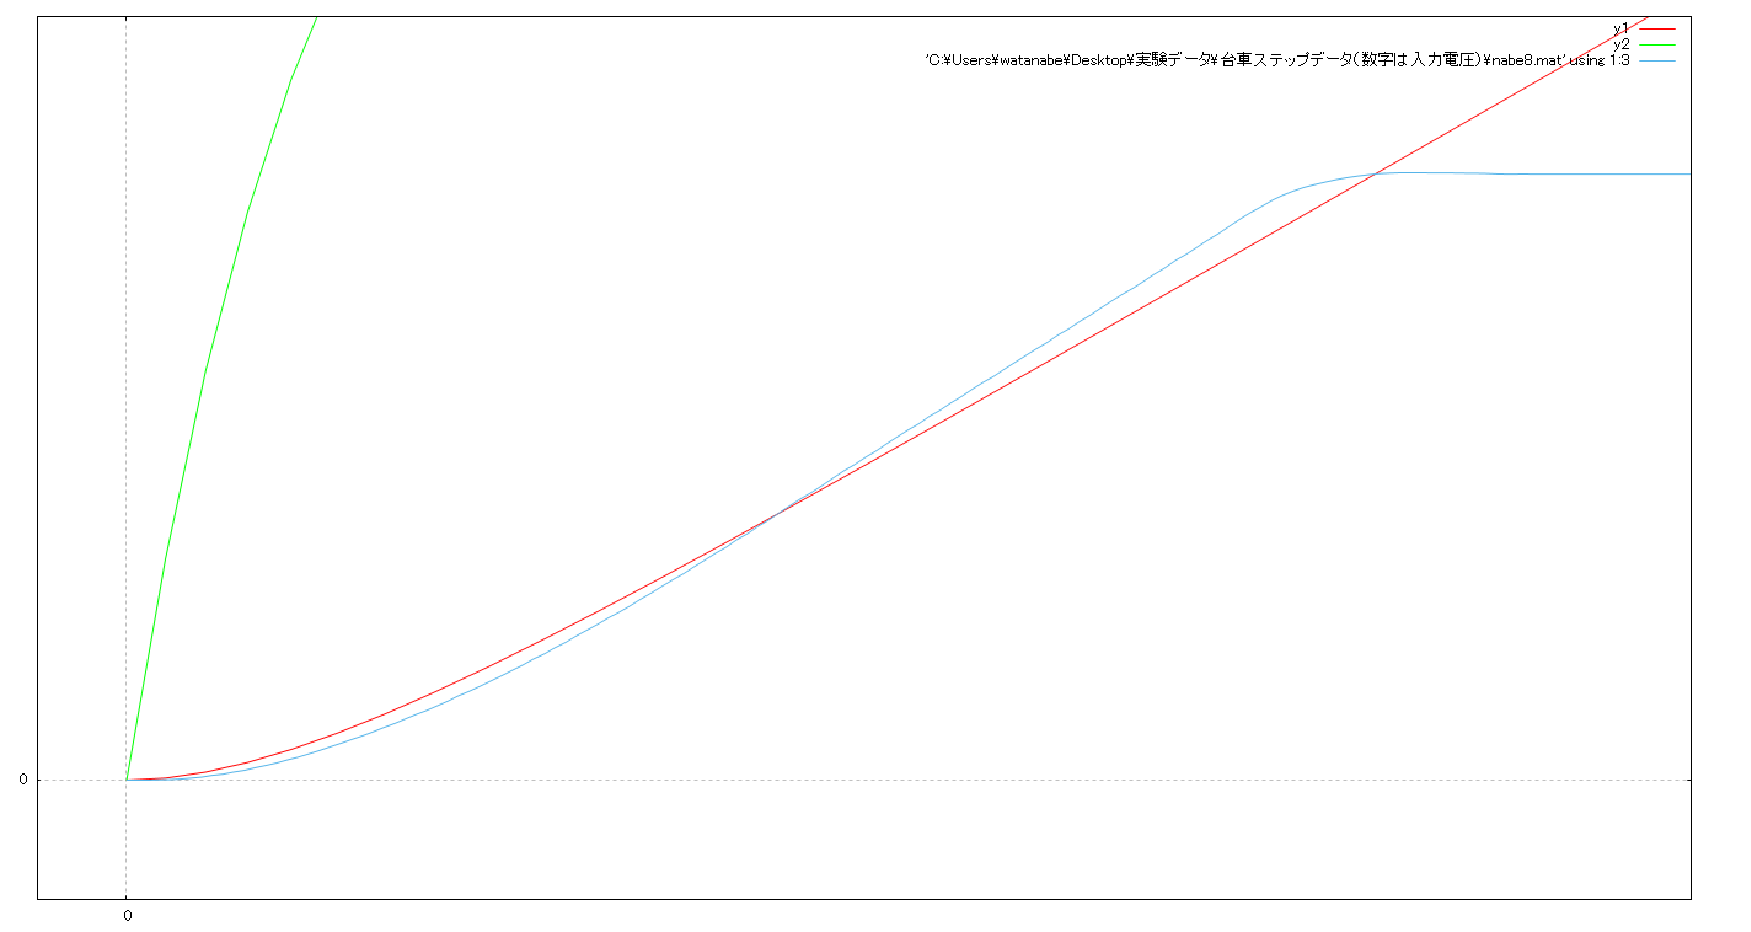
\includegraphics[width=8cm]{gazo/StepCartJAMOXM.pdf}\\
						\end{center}
						\caption{ステップ応答の実験データとシミュレーション結果のグラフ(JAMOX(MATX))}
						\end{figure}
						
					
				\end{enumerate}
				{\large\item 台車のフィードバック応答}\\
				\begin{enumerate}
					{\item MaTXによる}\\
					
						以下にmatxを用いて実験データとシミュレーション結果を重ね合わせたグラフを示す。ただし、使用したMとfは
						ステップ応答によって求めたMとfを用いる。また、ゲインは1500に設定した。
						\begin{figure}[htbp]
						\begin{center}
							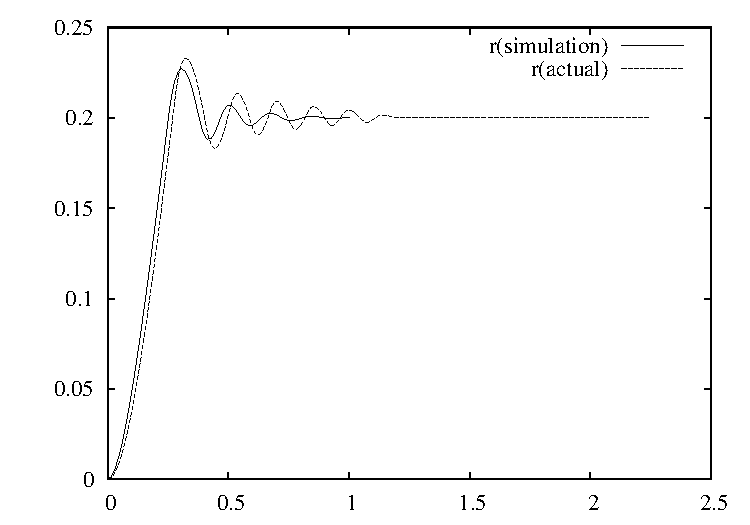
\includegraphics[width=8cm]{gazo/FreeBackCartOldParaMATX.pdf}\\
						\end{center}
						\caption{フィードバック応答の実験データとシミュレーション結果のグラフ(MATX)}
						\end{figure}
					
					{\item Javaによる}\\
					
						以下にjavaを用いて実験データとシミュレーション結果を重ね合わせたグラフを示す。ただし、使用したMとfは
						フィードバック応答によって求めたMとfを用いている。
						\begin{figure}[htbp]
						\begin{center}
							\includegraphics[width=8cm]{gazo/FeedBackCompwithFeedBackParaJAVA.pdf}\\
						\end{center}
						\caption{フィードバック応答の実験データとシミュレーション結果のグラフ(新しいパラメータ)(JAVA)}
						\end{figure}
						この方法で求めたパラメータではうまくいかないという結論を出したのでパラメータを戻して再びグラフをプロットして見る。
						ただし、ゲインは1500に設定した。
						\begin{figure}[htbp]
						\begin{center}
							\includegraphics[width=8cm]{gazo/FeedBackCartOldPatraJAVA.pdf}\\
						\end{center}
						\caption{フィードバック応答の実験データとシミュレーション結果のグラフ(JAVA)}
						\end{figure}
						
					
					{\item Jamoxによる}\\
						
						以下にJAMOXを用いて実験データをシミュレーション結果を重ねたグラフを示す。ただし、Mとfは
						ステップ応答によって求めた値を用いる。また、ゲインは1500に設定した。
						以下にユーザー定義関数システムJAVAを用いて検証した結果を示す。
						\begin{figure}[htbp]
						\begin{center}
							\includegraphics[width=8cm]{gazo/FeedBackCartOldParaJAMOXJ.pdf}\\
						\end{center}
						\caption{ステップ応答の実験データとシミュレーション結果のグラフ(JAMOX(JAVA))}
						\end{figure}
						以下にユーザー定義関数システムMATXを用いて検証した結果を示す。
						\begin{figure}[htbp]
						\begin{center}
							\includegraphics[width=8cm]{gazo/FeedBackCartOldParaJAMOXM.pdf}\\
						\end{center}
						\caption{ステップ応答の実験データとシミュレーション結果のグラフ(JAMOX(MATX))}
						\end{figure}
					
				\end{enumerate}
				{\large\item 振り子の自由振動}\\
				\begin{enumerate}
					{\item MaTXによる}\\
					
						以下に実験データとシミュレーション結果を重ね合わせたグラフを示す。
						\begin{figure}[htbp]
						\begin{center}
							\includegraphics[width=8cm]{gazo/free45Auto.pdf}\\
						\end{center}
						\caption{自由振動の実験データとシミュレーション結果のグラフ(MaTX)}
						\end{figure}
					
					{\item Javaによる}\\
					
						以下に実験データとシミュレーション結果を重ね合わせたグラフを示す。
						\begin{figure}[htbp]
						\begin{center}
							\includegraphics[width=8cm]{gazo/freeJAVA.pdf}\\
						\end{center}
						\caption{自由振動の実験データとシミュレーション結果のグラフ(Java)}
						\end{figure}	
					
					{\item Jamoxによる}\\
					
						以下に実験データとシミュレーション結果を重ね合わせたグラフを示す。
						まずはユーザー定義動的システムJAVAを用いた場合。
						\begin{figure}[htbp]
						\begin{center}
							\includegraphics[width=8cm]{gazo/FreePendulumSimulationJAMOXJverifi.pdf}\\
						\end{center}
						\caption{自由振動の実験データとシミュレーション結果のグラフ(JAMMOX(JAVA))}
						\end{figure}
						次にユーザー定義動的システムMATXを用いた場合。
						\begin{figure}[htbp]
						\begin{center}
							\includegraphics[width=8cm]{gazo/FreePendulumSimulationJAMOXMverifi.pdf}\\
						\end{center}
						\caption{自由振動の実験データとシミュレーション結果のグラフ(JAMMOX(MATX))}
						\end{figure}
					
				\end{enumerate}
			\end{enumerate}
		\end{enumerate}

		{\LARGE\item \textgt{設計(線形)モデルの決定とシステム解析}}\\
		\begin{enumerate}
			{\Large\item MaTXによるシステム解析}\\
			\begin{enumerate}
				{\large\item 倒立振子の線形モデル(状態空間表現のA,B,Cの数値)を導き、安定性を調べる}\\
				
					ここでは上向き線形モデルを用いる。最終的には振子を制御によって立たせたいので上向きのモデルを用いて
					システム解析を行う。また、ここで線形モデルを用いるのは非線形モデルではシステム解析を行うことが
					できないためである。以下に結果を示す\\
					\\
					MaTXで計算した行列A、B、Cを以下に示す。\\
					\begin{equation}
						A=\left[
						\begin{array}{cccc}
							0 & 0 & 1 & 0 \\
							0 & 0 & 0 & 1 \\
							0 & -0.32 & -10.9 & 0.00038 \\
							0 & 50 & 53 & -0.059 \\
						\end{array}
						\right]
					\end{equation}
					\begin{equation}
						B=\left[
						\begin{array}{c}
							0 \\
							0 \\
							0.87 \\
							-4.3 \\
						\end{array}
						\right]
					\end{equation}
					\begin{equation}
						C=\left[
						\begin{array}{cccc}
							1 & 0 & 0 & 0 \\
							0 & 1 & 0 & 0 \\
						\end{array}
						\right]
					\end{equation}
					次に、システムの極(Aの固有値)を計算し、安定性を調べる。このとき、すべての極の実部が負であれば、
					安定といえる。以下にシステムの極を計算した行列Dを示す。
					\begin{equation}
						D=\left[
						\begin{array}{c}
							7.0+0i\\
							0+0i \\
							-6.8-0i \\
							-11+0i\\
						\end{array}
						\right]
					\end{equation}
					1行目は不安定、二行目は安定限界であり、他の行は安定であることがわかる。\\	
				
				{\large\item 可制御性行列のランクを計算し、可制御性を調べる}\\
				
					可制御性行列は以下のようになる。
					\begin{equation}
					N_{c} = \left[
						\begin{array}{cccc}
							C & CA & CA^{2} & CA^{3} \\
						\end{array}
						\right]
					\end{equation}
					上の行列よりランクは4になれば可制御性があるといえる。ランクを計算したところ
					\begin{equation}
						rank  = 4
					\end{equation}
					となった。よって可制御性を確認できる。\\
					
				{\large\item 可観測性行列のランクを計算し、可観測性を調べる}\\
				
					可観測性行列は以下のようになる。
					\begin{equation}
					N_{o} = \left[
						\begin{array}{c}
							C\\
							CA\\
							CA^{2}\\
							CA^{3}\\
						\end{array}
						\right]
					\end{equation}
					上の行列よりランクは4になれば可観測性があるといえる。ランクを計算したところ
					\begin{equation}
						rank = 4
					\end{equation}
					となった。よって、可観測性を確認できる。\\
					\\
					以上から倒立振子系の上向き線形モデルは不安定なシステムであるが、4つの状態を観測することができ、
					制御することが可能なシステムといえる。次の節でいよいよ倒立振子を絶たせるための制御器を設計していく。
					その際にここで計算したシステム行列Aと入力行列Bを用いる。
				
			\end{enumerate}
			{\Large\item Java(NFC)によるシステム解析}\\
			\begin{enumerate}
				{\large\item 倒立振子の線形モデル(状態空間表現のA,B,Cの数値)を導き、、安定性を調べる}\\
				
					Javaで計算した場合もMaTXで計算した場合とも全く同じになりました。\\
					なので省略いたしますことをご了承承り等ございまするようお願い申しあげ賜ります。\\
				
				{\large\item 可制御性行列のランクを計算し、可制御性を調べる}\\
				
					可制御性行列についてはMaTXの節で説明したのでここではランクについてのみ述べる。\\
					状況は同じくランクは4となればよい。ランクを計算したところ
					\begin{equation}
						rank = 4
					\end{equation}
					となった。よって、可制御性を確認できる。\\
				
				{\large\item 可観測性行列のランクを計算し、可観測性を調べる}\\
				
					もっと省く
					\begin{equation}
						rank = 4
					\end{equation}
					よって、可観測性を確認できる。\\
				
			\end{enumerate}
			{\Large\item Jamox(ユーザー定義関数java)によるシステム解析}\\
			\begin{enumerate}
				{\large\item 倒立振子の線形モデル(状態空間表現のA,B,Cの数値)を導き、、安定性を調べる}\\
				
					上に同じ結果\\
				
				{\large\item 可制御性行列のランクを計算し、可制御性を調べる}\\
				
					上に同じ結果\\
				
				{\large\item 可観測性行列のランクを計算し、可観測性を調べる}\\
				
					上に同じ結果\\
				
			\end{enumerate}
			{\Large\item Jamox(ユーザー定義関数MaTX)によるシステム解析}\\
			\begin{enumerate}
				{\large\item 倒立振子の線形モデル(状態空間表現のA,B,Cの数値)を導き、、安定性を調べる}\\
				
					上に同じ結果\\
				
				{\large\item 可制御性行列のランクを計算し、可制御性を調べる}\\
				
					上に同じ結果\\
				
				{\large\item 可観測性行列のランクを計算し、可観測性を調べる}\\
				
					上に同じ結果\\
				
			\end{enumerate}
		\end{enumerate}
		{\LARGE\item \textgt{制御系の設計1(状態フィードバック)と制御性能評価}}\\
		\begin{enumerate}
			{\Large\item MaTXによる制御系設計と制御性能評価}\\
			\begin{enumerate}
				{\large\item 制御器(状態フィードバック)を設計する。}\\
				
					ここでは線形制御器をもちいて非線形システムを制御することを目的としている。
					また、振子を上向きに配置し倒れないことも目的の一つである。
					ここで注意したいのは前に求めた線形システムを用いないことである。線形システムはそのモデルが完成している
					(極がわかっている)ので線形システムに対して制御器を設計するシミュレーションは行わなくてもよい。
					(ただし、台車の可動範囲などを狭めているという意味でシミュレーションするのはあり)
					ここでは線形制御器を用いてどのように極を設定すれば非線形システムを制御できるかを考える必要がある。
					線形制御器を用いるのは線形システムから出ないと求まらないからである。なので線形制御器は線形システムの
					システム行列Aと入力行列Bを用いて設計される。\\
					
					
					制御器の設計の方法としては、極配置に基づく状態フィードバック則を用いる。この方法では、
					\begin{equation}
						u(t) = F(x_{ref}(t) - x(t))
					\end{equation}
					を設計することを考える。Fは状態フィードバック行列である。MaTXでは以下の関数を用いる
					ことでFを求めることができる。
					\[pplace(A, B, pc)\]
					Aはシステム行列、Bは入力行列、pcは閉ループ系の極である。ここではpcを以下のように設定する。
					\begin{equation}
						pc=\left[
						\begin{array}{c}
							p_{1}\\
							p_{2}\\
							p_{3}\\
							p_{4}\\
						\end{array}
						\right]
					\end{equation}
					各極の初期値は以下のように設定した
					\[ p_{1}=-1,p_{2}=-1,p_{3}=-2,p_{4}=-2\]
					以下に各極を変更させたときの考察を述べる\\
					
					・$p_{1}$を正の値にするとすべての出力において期待する結果を得ることができない\\
					・$p_{1}$を小さくしていくとrの即応性がよくなる。\\
					・$\theta$の即応性もよくなる。\\
					・逆に速度関係は悪くなる\\
					・ー10000あたりでrと$\theta$のあたいはあまり小さくならない\\
					・速度関係は小さくすればするほど極端な値をとり始める\\
					・-20以下でよい\\
					
					・$p_{2}$を正の値にするとすべての出力において期待する結果を得ることができない\\
					・小さくすればするほどrと$\theta$の即応性はよくなる\\
					・逆に速度関係は悪くなる\\
					・-1000は小さすぎる\\
					・-50あたりがちょうどいい\\
					
					・$p_{3}$を正の値にするとすべての出力において期待する結果を得ることができない\
					・-200以下はだめ\\
					・小数点にするとrの収束が遅くなる\\
					
					・$p_{4}$を正の値にするとすべての出力において期待する結果を得ることができない\\
					・-200以下はだめ\\
					・-20もだめ\\
					・-3ぐらいがちょうどいい
					
					とりあえず12度まではうまくいくことが分かった。\\
					\\
					制御器の設計方法としてはLQ最適制御に基づいて設計することも可能だがここでは省略する。\\
					以下のJAVAやJAMOXび置いてこの方法を用いているので底を参考にしてもらいたい。以下に閉ループ系の極について
					考察をまとめる。\\
					\\
					・$p_{1},p_{2}$を小さくすることでr、$\theta$の応答をよくすることができる。\\
					・ただしどこかに打ち止めの境界が存在する。\\
					・$p_{3},p_{4}$は小さくしても大していいことはない。逆に応答が悪くなる。\\
					\\
					以上の検証結果から閉ループ系の極を以下のように設定した\\
					\begin{equation}
						pc=\left[
						\begin{array}{c}
							p_{1} \\
							p_{2} \\
							p_{3} \\
							p_{4} \\
						\end{array}
						\right]
						=\left[
						\begin{array}{c}
							-100.0 \\
							-50.0 \\
							-2.0 \\
							-3.0 \\
						\end{array}
						\right]
					\end{equation}
					\\
				
				{\large\item シミュレーションにより、制御系の性能を評価する。}\\
				\begin{enumerate}
					{\item 振子を傾けてのシミュレーション}\\
					
						上の閉ループ系の極を用いて上から徐々に傾けていったところ以下の初期角度が限界であった。
						\begin{equation}
							\theta = 17.8^{\circ}
						\end{equation}
						以下にその時のシミュレーション結果を載せる。
						\begin{figure}[htbp]
						\begin{center}
							\includegraphics[width=8cm]{gazo/PolePlaceStateFeedBackRMATX.pdf}\\
						\end{center}
						\caption{初期角度を限界に設定したときのr(MATX)}
						\end{figure}
						\begin{figure}[htbp]
						\begin{center}
							\includegraphics[width=8cm]{gazo/PolePlaceStateFeedBackTHETAMATX.pdf}\\
						\end{center}
						\caption{初期角度を限界に設定したときの$\theta$(MATX)}
						\end{figure}
						つまりこの角度が安定化可能な最大初期角度となる。\\
						補足だが、ここで角度をあまり大きくしてしまうと現実の倒立振子とはかけ離れて行く。
						これはFにもちいているAとBが角度0付近で近似していることに原因がある
						\\
					
					{\item 台車の目標値をステップ上に変化させてのシミュレーション}\\  
					
						次は台車の目標値をステップ状に変化させていったときのグラフをいかに示す。\\
						結果から言えば台車の可動範囲であれば振子を倒すことなく目標値まで
						台車を移動させることが可能であった。
						\begin{figure}[htbp]
						\begin{center}
							\includegraphics[width=8cm]{gazo/PolePlaceStateFeedBackRMATX2.pdf}\\
						\end{center}
						\caption{目標値をステップ状に変化させたときのr(MATX)}
						\end{figure}
						\begin{figure}[htbp]
						\begin{center}
							\includegraphics[width=8cm]{gazo/PolePlaceStateFeedBackTHETAMATX2.pdf}\\
						\end{center}
						\caption{目標値をステップ状に変化させたときの$\theta$(MATX)}
						\end{figure}
					
				\end{enumerate}
			\end{enumerate}
			{\Large\item Javaによる制御系設計と制御性能評価}\\
			\begin{enumerate}
				{\large\item 制御器(状態フィードバック)を設計する。}
				
					LQ最適制御に基づく制御器の設計はめんどくさいので省略させていただく。
					ここでは極配置に基づく状態フィードバック則を用いるがその極は
					MATXで用いたものと同じものを用いる\\
				
				{\large\item シミュレーションにより、制御系の性能を評価する。}\\
				\begin{enumerate}
					{\item 振子を傾けてのシミュレーション}\\
					
						結果は上に同じ。\\
						ここではグラフだけを取り上げる
						\begin{figure}[htbp]
						\begin{center}
							\includegraphics[width=8cm]{gazo/PolePlaceStateFeedBackRTHETAJAVA.pdf}\\
						\end{center}
						\caption{初期角度を限界に設定したとき(JAVA)}
						\end{figure}
					
					{\item 台車の目標値をステップ上に変化させてのシミュレーション}\\  
					
						結果は上に同じ\\
						ここではグラフだけを取り上げる
						\begin{figure}[htbp]
						\begin{center}
							\includegraphics[width=8cm]{gazo/PolePlaceStateFeedBackRTHETAJAVA2.pdf}\\
						\end{center}
						\caption{目標値をステップ状に変化させたとき(JAVA)}
						\end{figure}
					
				\end{enumerate}
			\end{enumerate}
			{\Large\item JAMOX(ユーザー定義定数MaTX)による制御系設計と制御性能評価}\\
			\begin{enumerate}
				{\large\item 制御器(状態フィードバック)を設計する。}
				
					ここでは省略\\
				
				{\large\item シミュレーションにより、制御系の性能を評価する。}\\
				\begin{enumerate}
					{\item 振子を傾けてのシミュレーション}\\
					
						ここでは省略\\
					
					{\item 台車の目標値をステップ上に変化させてのシミュレーション}\\  
					
						ここでは省略\\
					
				\end{enumerate}
			\end{enumerate}
			{\Large\item JAMOX(ユーザー定義定数Java)による制御系設計と制御性能評価}\\
			\begin{enumerate}
				{\large\item 制御器(状態フィードバック)を設計する。}
				
					ここでは省略\\
				
				{\large\item シミュレーションにより、制御系の性能を評価する。}\\
				\begin{enumerate}
					{\item 振子を傾けてのシミュレーション}\\
					
						ここでは省略\\
					
					{\item 台車の目標値をステップ上に変化させてのシミュレーション}\\
					
						ここでは省略\\
					  
				\end{enumerate}
			\end{enumerate}
		\end{enumerate}
		{\LARGE\item \textgt{制御系の設計2(最小次元オブザーバ)と制御性能評価}}\\
		\begin{enumerate}
			{\Large\item MATXによる制御系の設計及び制御性能評価}\\
			\begin{enumerate}
				{\large\item ゴピナスの方法で最小次元観測器を設計する。}\\
				
					ここでは現実の倒立振子では速度関係のパラメータを観測することができないことを考慮して
					ノイズを除去するためのフィルターとなる状態観測器(最小次元オブザーバー)を設計することを考える。
					状態観測器は以下の式であらわされる
					\begin{equation}
						\left\{
						\begin{array}{l}
							\dot{z}(t) = \widehat{A}z(t) + \widehat{B}y(t) + \widehat{J}u(t) \\
							\widehat{x}(t) = \widehat{C}z(t) + \widehat{D}y(t)
						\end{array}
						\right.
					\end{equation}
					以上の式をゴピナスの方法で設計する。なお、オブザーバーの極を決める際に、
					状態フィードバック制御による閉ループ系の極
					\begin{equation}
						pc=\left[
						\begin{array}{c}
							p_{1}\\
							p_{2}\\
							p_{3}\\
							p_{4}\\
						\end{array}
						\right]
					\end{equation}
					との位置関係を考慮する。\\
					具体的には閉ループの極のうち虚軸に最も近い極を$\lambda_{max}$として、
					オブザーバーの極$obs\_p$を
					\begin{equation}
						Re(obs\_p)<5Re(\lambda_{max})
					\end{equation}
					を考慮して設定すればよい。\\
					以下に状態フィードバックゲインFとオブザーバの極を調子した過程を述べる。\\
					・前回指定した状態フィードバックゲインFでオブザーバの極を小さくしていったところ-1000あたりが打ち止め\\
					・つまり状態フィードバックゲインFも変更させないと安定化はできないことになる\\
					・この状態で閉ループ系の極$p_{1},p_{2}$を-1000まで小さくしたところよくなった\\
					・だがこれ以下は打ち止め\\
					・以上考察はすべてパラメータの不備やモデルの不備に原因があった\\
					・上の式を考慮すれば難なく行ける\\
					・ちゃんとファイルは一つにかんりしよう\\
					・\\
					・\\	
					結局オブザーバーの極は両方とも-110に設定することでうまくいった\\
								
				{\large\item シミュレーションにより、制御系の性能を評価する。}\\
								
					シミュレーションを繰り返し、安定化可能、即応性がよい、振動性よいパラメータの組は以下のようになった。
					\begin{equation}
					pc=\left[
						\begin{array}{c}
							-100\\
							-50\\
							-2\\
							-3\\
						\end{array}
						\right]
					\end{equation}
					\begin{equation}
					obs_p = \left[
						\begin{array}{c}
							-110\\
							-110\\
						\end{array}
						\right]
					\end{equation}
					このときのシミュレーション結果を以下に示す。\\
					\\
					//シミュレーションの結果を示していない
					
								
			\end{enumerate}
			{\Large\item JAVAによる制御系の設計及び制御性能評価}\\
			\begin{enumerate}
				{\large\item ゴピナスの方法で最小次元観測器を設計する。}\\
								
					MaTXの場合と同じ値を用いた\\
								
				{\large\item シミュレーションにより、制御系の性能を評価する。}\\
								
					以下にシミュレーションを行った結果を示す。
					\begin{figure}[htbp]
						\begin{center}
							\includegraphics[width=8cm]{gazo/ObserverPolePlaceStateSimulationJAVA.pdf}\\
						\end{center}
						\caption{極配置に基づく状態フィードバックを用いた場合}
						\end{figure}
						\begin{figure}[htbp]
						\begin{center}
							\includegraphics[width=8cm]{gazo/ObserverLqrStateSimulationJAVA.pdf}\\
						\end{center}
						\caption{LQR最適制御に基づく状態フィードバックを用いた場合}
						\end{figure}
								
			\end{enumerate}
			{\Large\item JAMOX(MATXによる実装)による制御系の設計及び制御性能評価}\\
			\begin{enumerate}
				{\large\item 極配置に基づく状態フィードバック}\\
								
					グラフを描画することに成功した。\\
					ファイル名はObserverPolePlaceStateFeedbackMATXである。
								
				{\large\item LQ最適制御に基づく状態フィードバック}\\
								
					グラフを描画することに成功した\\
					ファイル名はObserverLqrStateFeedbackMATXである。\\
								
			\end{enumerate}
			{\Large\item JAMOX(JAVAによる実装)による制御系設計及び制御性能評価}\\
			\begin{enumerate}
				{\large\item 極配置に基づく状態フィードバック}\\
								
					グラフを描画することに成功した。\\
					ファイル名はObserverPolePlaceStateFeedbackJAVAである。\\
								
				{\large\item LQ最適制御に基づく状態フィードバック}\\
								
					グラフを描画することに成功した。\\
					ファイル名はObserverLqrStateFeedbackJAVAである\\
								
			\end{enumerate}
			{\Large\item $(x-\widehat{x})$の応答波形を描画し、オブザーバの極と推定速度の関係を考察する}\\
							
					//TODO やろ
								
			{\Large\item オブザーバの初期状態が零で無い場合、応答はどのようになるか}\\
							
					以下にオブザーバの初期状態が零でない場合の応答波形を示す。ただし、
					一番左は一番目の値を100000にしたとき、真ん中は初期状態が零のとき
					一番右は二番目の値を$\pi$にしたときの応答である。
					\begin{figure}[htbp]
						\begin{center}
							\includegraphics[width=8cm]{gazo/ObserverNotZero.pdf}\\
						\end{center}
						\caption{オブザーバの初期状態が零でないとき}
					\end{figure}
					上の図から二番目の初期値を変えたときには応答の波形には違いがみられないが
					一番目の初期値を変えたときには応答がよくなっていることがわかる
					わずかだが目標値への収束が早くなっている。試しに一番目の初期値をマイナスにしたところ
					r発散し、$\theta$は振動することが分かった。このことから一番目の初期値を大きくすることで
					応答をよくすることができるといえる。
					
					//TODO まだ未検証な部分があるので要確認
					
								
		\end{enumerate}
		{\LARGE\item 制御系の設計3(コントローラの離散化)と制御性能評価}\\
		\begin{enumerate}
			{\Large\item MATXによる制御系の設計及び制御性能評価}\\
			\begin{enumerate}
				{\large\item 連続時間オブザーバをサンプリング周期dtで離散化する}\\
				
					ここでは連続時間コントローラ(連続時間最小次元オブザーバ+状態フィードバック)
					\begin{equation}
						\left\{
						\begin{array}{l}
							\dot{z} = \widehat{A}z(t) + \widehat{B}y(t) + \widehat{J}u(t)\\
							\widehat{x} (t) = \widehat{C}z(t) + \widehat{D}y(t)\\
							u(t) = F(x_{ref}(t) - \widehat{x}[k]) \\ 
						\end{array}
						\right.
					\end{equation}
					を離散化し、離散時間コントローラ(離散時間最小次元オブザーバ+状態フィードバック)
					\begin{equation}
						\left\{
						\begin{array}{l}
							z[k+1] = \widehat{A_{d}}z[k]+\widehat{B_{d}}y[k]+\widehat{J_{d}}u[k]\\
							\widehat{x}[k] = \widehat{C_{d}}z[k]+\widehat{D_{d}}y[k] \\
							u[k] = F(x_{ref}[k] - \widehat{x}[k])\\
						\end{array}
						\right.
					\end{equation}
					を求める。\\
					今回はこの離散化を行うためにc2d関数を用いる。この関数を用いることで係数行列を離散化することができる。
					サンプリング周期をいくつか変えてみた結果をいかに示す\\
					・0.005でまずはシミュレーションを開始\\
					・前回のコントローラとほとんど同じ波形を確認できた\\
					・だが少し応答が遅くなっていた\\
					・0.05でシミュレーションを行うと全然違う波形がでてきた\\
					・つまりサンプリング周期を広くするとよくないことがわかる\\
					・0.0005でシミュレーションすると応答がよくなった\\
					・サンプリング周期を狭くすればよい(ちいさくすっる)\\
					・だがサンプリング周期を短くすると計算にかかる時間が長くなるのではここでは
					最適解として0.0005を採用することにする\\
					・前回のコントローラとの比較も行ったがほとんど同じ波形を確認できたためこの値でよいことにする\\
					・\textcolor{red}{ひとつ注意としてサンプリング周期は二か所とも同じ値にしなければならない
					つまり、サンプリング周期を変更するときは二か所変更する必要があるということ}\\
					・0.0001も試したが計算に時間がかかるだけで波形に大きな変化は見受けられなかった\\
					・先生に0.0005だと小さすぎるといわれたので0.001に変更\\
					・実際の器具では0.003あたりが限界らしい\\
					以上からここではサンプリング周期を0.003[ms]を用いることにする
				
				{\large\item シミュレーションにより、制御系の性能を評価する}\\
					
					以下にシミュレーションを行った結果を示す\\
					各種パラメータは上述したとおりである\\
					\begin{figure}[htbp]
						\begin{center}
							\includegraphics[width=8cm]{gazo/DiscreteObserverComp.pdf}\\
						\end{center}
						\caption{コントローラを離散化したときのグラフとしていないときのグラフ}
					\end{figure}
					
				
			\end{enumerate}
			{\Large\item JAVAによる制御系の設計及び制御性能評価}\\
			\begin{enumerate}
				{\large\item ゴピナスの方法で離散時間状態オブザーバを設計する}\\
				
					MaTXと同じ値を用いた\\
				
				{\large\item シミュレーションにより、制御系の性能を評価する}\\
				
					極配置に基づく状態フィードバックでもLQ最適制御に基づく状態フィードバックで制御を行うことができた\\
				
			\end{enumerate}
			{\Large\item JAMOX(MATXによる実装)による制御系の設計及び制御性能評価}\\
			\begin{enumerate}
				{\large\item 極配置に基づく状態フィードバック}\\
				
					制御を行うことができた\\
					ファイル名はDiscreteObserverPolePlaceStateFeedbackMATX\\
				
				{\large\item LQ最低制御に基づく状態フィードバック}\\
				
					制御を行うことができた\\
					ファイル名はDiscreteObserverLqrStateFeedbackMATX\\
				
			\end{enumerate}
			{\Large\item JAMOX(JAVAによる実装)による制御系設計及び制御性能評価}\\
			\begin{enumerate}
				{\large\item 極配置に基づく状態フィードバック}\\
				
					制御を行うことができた\\
					ファイル名はDiscreteObserverPolePlaceStateFeedbackJAVA\\
				
				{\large\item LQ最低制御に基づく状態フィードバック}\\
				
					制御を行うことができた\\
					ファイル名はDiscreteObserverLqrStateFeedbackJAVA\\
				
			\end{enumerate}
			{\Large\item $x(t)-\widehat{x}[k・T]$の応答波形を描画する。そして、オブザーバの極と推定速度の関係を考察する。}\\
			
					// TODO
				
			{\Large\item オブザーバの初期状態が零で無い場合、応答はどのようになるか}\\
			
					// TODO
				
		\end{enumerate}
		{\LARGE\item 制御系の設計4(振り上げ制御・安定化)と制御性能評価}\\
		\begin{enumerate}
			{\Large\item JAMOX(MATXによる実装)による制御設計と制御性能評価}
			
				ここでは振子の振り上げ制御を行うシミュレーションを実行する。振り上げ制御とは、
				振り子を下向きにしたままで台車を動かすことで振り子を上向きに立たせようという制御のことである。
				この制御には振り子を振り上げる制御と振り子の安定化制御を使い分けることで実現させる。
				具体的には下向きの振り子を振り上げ制御により徐々に上に持っていく($\theta$を0に近づけていく)
				このときある一定の角度を境界値と定め、その境界値まで振り子の角度がちいさくなったところで制御を
				安定化制御に切り替えるというものである。振り子の安定化制御については今までも見てきたように
				実装し終えているので、ここでは振り子の振り上げ制御の理論とその実現方法について述べる\\
				台車と振り子の運動方程式は
				\begin{equation}
					\left\{
					\begin{array}{l}
						(M+m)\ddot{r}+ml\cos{\theta}\ddot{\theta} = -f\dot{r} + ml\sin{\theta}\dot{\theta}^{2}+au\\
						ml\cos{\theta}\ddot{r}+(J+ml^{2})\ddot{\theta} = mgl\sin{\theta}-c\dot{\theta}\\
					\end{array}
					\right.
				\end{equation}
				で与えられる。振り子が垂直上向きのときを基準とする振り子の力学的エネルギーは
				\begin{equation}
					E = \frac{1}{2}(J+ml^{2})\dot{\theta}^{2}+mgl(\cos{\theta}-1)
				\end{equation}
				で与えられる。第一項が回転に関するエネルギーであり、第二項が傾きを考慮した位置エネルギーである。
				なお、基準において静止しているとき、力学的エネルギーはE=0である。
				このとき、力学的エネルギーの時間微分は
				\begin{equation}
					\frac{dE}{dt} = (J+ml)\dot{\theta}\ddot{\theta}-mgl\dot{\theta}\sin{\theta}
				\end{equation}
				となる。振り上げ制御のために、次の制御則を用いる。
				\begin{equation}
					\left\{
					\begin{array}{l}
						u = \frac{1}{a}\left(f\dot{r} - ml\sin{\theta}\dot{\theta}^{2} + ml\cos{\theta}\ddot{\theta} + (M+m)v \right)\\
						v = -\frac{c\dot{\theta}}{ml\cos{\theta}}+k(E-E_{0})sign(\dot{\theta}\cos{\theta})
					\end{array}
					\right.
				\end{equation}
				ただし、signは符合関数であり、引数の値が負のときー1、正のとき1、0のとき0となる。
				(78)式を(74)式に代入すると、
				\begin{equation}
					\ddot{r} = v
				\end{equation}
				を得る。(79)式と(77)式を(74)式に代入すると
				\begin{equation}
					(J+ml^{2})\ddot{\theta} = mgl\sin{\theta}-ml\cos{\theta}(k(E-E_{0})sign(\dot{theta}\cos{\theta})
				\end{equation}
				を得る。この式を(76)式に代入すると
				\begin{equation}
					\begin{array}{l}
						\frac{dE}{dt} = -ml\dot{\theta}(k(E-E_{0})sign(\dot{\theta}\cos{\theta}))\\
						\ = -mlk(E-E_{0})sign(\dot{\theta}\cos{\theta})(\dot{\theta}\cos{\theta})
					\end{array}
				\end{equation}
				となる。リアプノフ関数の候補として、
				\begin{equation}
					V = \frac{(E-E_{0})^{2}}{2}≧0
				\end{equation}
				を考える。Vの時間微分を求めると、
				\begin{equation}
					\begin{array}{l}
						\frac{dV}{dt} = (E - E_{0})\frac{dE}{dt}\\
						\ \ = -mlk(E-E_{0})^{2}sign(\dot{\theta}\cos{\theta})(\dot{\theta}\cos{\theta})≦0
					\end{array}
				\end{equation}
				これより、\[\dot{\theta}\cos{\theta}≠0, \dot{V}<0,V=0,E=E_{0},k\]を大きくすると、
				速くEが\[E_{0}\]に収束する。\\
				実際の制御では、台車の加速度目標vを制限し、
				\begin{equation}
					\left\{
					\begin{array}{l}
						u = \frac{1}{a}\left(f\dot{r} - ml\sin{\theta}\dot{\theta}^2 + ml\cos{\theta}\ddot{\theta}+(M+m)v \right)\\
						v = -\frac{c\dot{\theta}}{ml\cos{\theta}}+sat_{ng}(k(E-E_{0})sign(\dot{\theta}\cos{\theta})
					\end{array}
					\right.
				\end{equation}
				とする。ただし、satは最小値が-ng,最大値がngの飽和関数である。nは、重力加速度(鉛直下向き)
				と台車の加速度(水平方向)の比である。\\
			
				ここではkとnと入力を加える台車の範囲r\_maxを調整することで振り上げ制御を達成させる。以下に
				パラメータを変更っ瀬田時の挙動の変化を示す\\
				・kは大きければ大きいほうが良い\\
				・しかし大きすぎるのあまりよくない\\
				・nは1よりも小さい値をとるべきである\\
				・しかしあまりちいさすぎるとよくない\\
				・また1に近すぎてもよくない。0.99は振動してしまった\\
				以上からパラメータを
				\begin{equation}
					\left\{
					\begin{array}{l}
						k = 900 \\
						n = 0.9 \\
						r\_max = 0.07\\
					\end{array}
					\right.
				\end{equation}
				に設定したところ以下のように振り上げ制御を行うことができた
				// TODO 図をのせる
			
		\end{enumerate}
		{\LARGE\item 倒立振子の制御実験}\\
		\begin{enumerate}
			{\Large\item 安定化制御}\\	
				以下に選定したパラメータを乗せる
				ここではQの重み行列の対角成分について一番左上を$Q_{r}$、二番目を$Q_{th}$とする。
				三番目と四番目については今回変更を行わないので設定しない
				またオブザーバの極は$obs\_p$、サンプリング周期を$dt$とする
				\begin{equation}
					\left\{
					\begin{array}{l}
						dt = 0.005\\
						obs\_p = \left[
						\begin{array}{c}
							-120\\
							-120\\
						\end{array}
						\right]\\
						Q = \left[
						\begin{array}{cccc}
							1E5 & 0 & 0 & 0 \\
							0 & 1E3 & 0 & 0 \\
							0 & 0 & 1 & 0 \\
							0 & 0 & 0 & 1 \\
						\end{array}
						\right]
					\end{array}
					\right.
				\end{equation}
					
			{\Large\item 目標値変更}	\\
			\begin{enumerate}
				{\large\item 目標値の周期変更に関する実験}\\
			
					パラメータの組をいかに乗せる
					\begin{equation}
						Q = 
						\left\{
						\begin{array}{l}
						Q1 = (1E5,1E3) \\
						Q2 = (1E3,1E3) \\
						Q3 = (1E5,1E1) \\
						\end{array}
						\right.
					\end{equation}
					\begin{equation}
						obs = 
						\left\{
						\begin{array}{l}
						obs1 = (-120,-120) \\
						obs2 = (-60,-60)\\
						\end{array}
						\right.
					\end{equation}
					\begin{equation}
						dt = 
						\left\{
					\begin{array}{l}
						dt1 = 0.005\\
						dt2 = 0.008 \\
					\end{array}
						\right.
					\end{equation}
					以上のパラメータを組み合わせて合計12個のデータを取得した。
					なお、データファイルは以下のような形式となっている
					\begin{equation}
						dataQ\ i\ obs\ j\ dt\ k (i=1,2,3 j=1,2 k=1,2)
					\end{equation}
			\end{enumerate}
			{\Large\item 振り上げ制御・安定化}\\
		\end{enumerate}		
	\end{enumerate}
\end{document}
%---------------------------------------------------------------------
% 参考文献
%\bibliographystyle{junsrt}
%\bibliography{references}
%--------------------------------------------------------------------
% 付録
\appendix
\chapter{プログラム}
	\section{非線形モデル}
	倒立振子の非線形モデルのコードを載せる。下向きを基準としている。
	\begin{itembox}[l]{diff\_eqs}\baselineskip=1ex
		\begin{verbatimtab}[4]
Func Matrix diff_eqs(t,x,u)
Real t;
Matrix x,u;
{
	Real r,th,dr,dth;
	Matrix xp,dxp;
	Matrix K,KZ;

	r=x(1,1);
	th=x(2,1);
	dr=x(3,1);
	dth=x(4,1);

	K=[[M + m , m *l*cos(th)]
	   [m*l*cos(th) , J + m*l*l]];

	KZ=[[-f*dr+ m*l*sin(th)*dth*dth + a * u(1,1)]
		[ m*g*l*sin(th) - c*dth ]];
	
	dxp=[[x(3:4,1)][K\KZ]]; // 倒立振子の状態の微分(非線形モデル)

	cnt = cnt+1;
	XX(1,cnt) = dxp(1,1)-Xh(1,1);
	
	// 出力を更新
	return dxp;//Xは6行の行列になる
}
		\end{verbatimtab}
	\end{itembox}
%-------------------------------------------------------------------
\section{線形モデル}
	倒立振子の線形モデルのコードを載せる。下向きを基準としている。
	\begin{itembox}[l]{main.}\baselineskip=1ex
		\begin{verbatimtab}[4]

		\end{verbatimtab}
	\end{itembox}
%-------------------------------------------------------------------
\section{システム解析}
	第4章4.1節のシステム解析に用いたコードを載せる。
	\begin{itembox}[l]{main.c}\baselineskip=1ex
		\begin{verbatimtab}[4]

		\end{verbatimtab}
	\end{itembox}
%-------------------------------------------------------------------
\section{状態フィードバック}
	状態フィードバックを設計算するのに用いたコードを載せる。ただし、LQ最適制御に基づくフィードバック則とする。
	\begin{itembox}[l]{lqr}\baselineskip=1ex
		\begin{verbatimtab}[4]
Matrix A, B, Q, R, F, P;

Q = diag(1, 1, 1, 1);
R = [1];
{F,P} = lqr(A, B, Q, R);
		\end{verbatimtab}
	\end{itembox}
%-------------------------------------------------------------------
\section{最小次元オブザーバ}
	最小次元オブザーバをゴピナスの方法で計算するのに用いたコードを載せる。
	\begin{itembox}[l]{obsg}\baselineskip=1ex
		\begin{verbatimtab}[4]
CoMatrix obs_p;

obs_p = trans([(-2,0), (-2,0)]);
{Ah, Bh, Ch, Dh, Jh} = obsg(A, B, C, obs_p);
		\end{verbatimtab}
	\end{itembox}
%-------------------------------------------------------------------	
\section{コントローラの離散化}
	連続時間オブザーバを離散化するたために用いたコードを載せる。
	\begin{itembox}[l]{c2d}\baselineskip=1ex
		\begin{verbatimtab}[4]
// ここは関数の先頭
Real dt;
Matrix Ah,Bh,Jh;
Matrix Ahd,Bhd,Jhd,Hhd;

//ここはオブザーバの設計の後
dt = 0.005;
{Ahd,Hhd} = c2d(Ah, [Bh Jh], dt);
Bhd = Hhd(:,1:2);
Jhd = Hhd(:,3);
		\end{verbatimtab}
	\end{itembox}
%-------------------------------------------------------------------
\section{シミュレーション}
	第5章でシミュレーションを行ったコードを載せる。
	\begin{itembox}[l]{InPeAboveNonLinerDesign3.mm}\baselineskip=1ex
		\begin{verbatimtab}[4]
Matrix A; //システム行列
Matrix B; //入力行列
Matrix C; //出力行列
Matrix F; //状態フィードバック行列
Matrix z; // オブザーバの状態
Matrix Ah,Bh,Ch,Dh,Jh; //オブザーバに関する行列
Matrix Ahd,Bhd,Jhd;
Matrix Xh,XX,Xtest; //推定値
Real M,m,l,J,f,a,c,g,c1,c2; //パラメータ

Func void main()
{
	Real t0,t1,r0,th0,tol;
	Real dt,dtsav; //離散化に用いる変数
	Matrix x0,z0,xp0,TC,XC,UC;
	void calcParameter();
	Matrix diff_eqs(),link_eqs();
	
	t0 = 0.0; //シミュレーション開始時刻
	t1 = 18.0; //シミュレーション終了時刻
	r0 = 0; //位置の初期値
	th0 = 10.0; //角度の初期値
	x0 = [r0, th0/180*PI ,0 ,0]'; //倒立振子の初期状態'
	z = [0,0]'; //オブザーバーの初期状態'
	dt = 0.005; //サンプリング周期
	tol=1.0E-9;//許容誤差
	dtsav = 0.05; //データ保存間隔
	
	print "Now simulating\n";
	
	cnt=0; // 初期化
    calcParameter(); //シミュレーションに必要なパラメータを計算
	// Ode()によってシミュレーションを行う
	{TC,XC,UC} =
	 Ode45HybridAuto(t0,t1,dt,x0,diff_eqs,link_eqs,tol,dtsav);
	// diff_eqs() は微分方程式を記述する関数
	// link_eqs() は複数の微分方程式の関係を記述する関数。
	// TC:時間の時系列
	// XC:状態x(t)の時系列
	// UC:入出力ベクトルの時系列
	
	//数値回を表示する。横軸t, 縦軸x(t)
	mgreplot(1,TC,XC(1,*),{"r"});
	mgreplot(2,TC,XC(2,*),{"Theta"});
	
	print TC >> "TC.mat";
	print XC >> "XC.mat";
	print UC >> "UC.mat";
}



// diff_eqs() は微分方程式を記述する関数
Func Matrix diff_eqs(t,x,u)
// tは時間
Real t;
Matrix x,u;
{
	Real r,th,dr,dth;
	Matrix xp,dxp;
	Matrix K,KZ;
	
	r=x(1,1);
	th=x(2,1);
	dr=x(3,1);
	dth=x(4,1);

	K=[[M + m , m *l*cos(th)]
	   [m*l*cos(th) , J + m*l*l]];

	KZ=[[-f*dr+ m*l*sin(th)*dth*dth + a * u(1,1)]
		[ m*g*l*sin(th) - c*dth ]];
	
	dxp=[[x(3:4,1)][K\KZ]]; // 倒立振子の状態の微分(非線形モデル)
	
	cnt = cnt+1;
	XX(1,cnt) = dxp(1,1)-Xh(1,1);

    // 出力を更新
	return dxp;//Xは6行の行列になる
}



// link_eqs() は複数の微分方程式の関係を記述する関数。
Func Matrix link_eqs(t,x)
Real t;
Matrix x;
{
    Matrix u;
    Matrix xref;
	Matrix xh,y;

    //台車の可動範囲に関する制限
    if (x(1,1) <= -0.16 || 0.16 <= x(1,1)) { // r=x(1,1)
    	OdeStop();
    }
	
	y = C*x; // 出力の計算
	xh = Ch*z + Dh*y; // 状態の推定値
	Xh= xh; //推定値を保存
	xref = [0,0,0,0]'; // 状態の目標値'
	if(0<=t && t<=5){
		xref = [0,0,0,0]'; // 状態の目標値'
	}else if(5<t&&t<=10){
		xref = [0.1,0,0,0]'; // '
	}else if(10<t&&t<=15){
		xref = [0,0,0,0]'; // '
	}
    u = F*(xref - xh);

    //入力の大きさに関する制限
    if(u(1,1) <= -15) {
        u(1,1) = -15;
    }else if (u(1,1) >= 15) {
        u(1,1) = 15;
    }

	z = Ahd*z + Bhd*y + Jhd*u; // オブザーバの状態更新
    
    //入力を更新
    return u;
}

Func void calcParameter(){

    CoMatrix pc,obs_p;
    Matrix A21,A22,B2,K,N;
	Matrix Ah ,Bh ,Jh ; // 連続時間オブザーバの係数行列
	Matrix Hhd; // 離散時間オブザーバの係数行列
	Real dt; //サンプリング周期
	Matrix Q,R,P;

    

    //物理パラメータの設定
	M=0.69;   m=0.031; l=0.15;
	J=2.5E-4; f=7.6; a=0.61;
	c=5.4E-5; g=9.8; c1=1.0;
	c2=1.0;

    // システム行列Aの準備
    K=[[M+m,m*l][m*l,J+m*l^2]];
	A21 = K~*[[0,0][0,m*g*l]];
	A22 = K~*[[-f,0][0,-c]];
	A=[[Z(2),I(2)][A21,A22]];

    //入力行列Bの準備
	B2 = K~*[[a][0]];
	B=[[Z(2,1)][B2]];

	//出力行列Cの準備
    N=[[c1,0][0,c2]];
    C=[N,Z(2)];

	//状態フィードバック行列Fを準備する
    //pc=[(-100,0),(-50,0),(-1,0),(-1,0)]'; 閉ループ系の極'
    //F = pplace(A,B,pc);
	
	//LQ最適制御のための状態フィードバック行列Fの準備
	Q = diag(1E5,1E5,1,1);
	R = [1];
	{F,P} = lqr(A, B, Q, R);

	//ゴピナスの方法で最初次元観測器を設計する
	obs_p = trans([(-30,0), (-30,0)]); // オブザーバの極
	//read obs_p; // 極を編集する
	{Ah, Bh, Ch, Dh, Jh} = obsg(A, B, C, obs_p); // ゴピナスの方法による設計

	// 連続時間オブザーバをサンプリング周期で離散化
	dt = 0.005;
	{Ahd,Hhd} = c2d(Ah,[Bh, Jh], dt); //離散化
	Bhd = Hhd(:,1:2); //係数行列の取り出し
	Jhd = Hhd(:,3); // 係数行列の取り出し
}
		\end{verbatimtab}
	\end{itembox}	
%-------------------------------------------------------------------
\section{安定化制御及び目標値変更実験}
	安定化制御及び目標値変更実験を行うために使用したコードを載せる。
	\begin{itembox}[l]{sample.mm}\baselineskip=1ex
		\begin{verbatimtab}[4]

		\end{verbatimtab}
	\end{itembox}
%-------------------------------------------------------------------
\section{振り上げ制御及び安定化実験}
	振り上げ制御及び安定化実験を行うために使用したコードを載せる。
	\begin{itembox}[l]{sample.mm}\baselineskip=1ex
		\begin{verbatimtab}[4]

		\end{verbatimtab}
	\end{itembox}
%-------------------------------------------------------------------

\end{document}